% !TeX program = xelatex
% !BIB program = biber
%%%%%%%%%%%%%%%%%%%%%%%% TEMPLATE INFO %%%%%%%%%%%%%%%%%%%%%%%%%%%%%%
%:     Template Name = cpe-thesis-th
%:     Version Name  = th-vectier-1.1
%:     Created by:
%:       - Peerapon Siripongwutikorn (peerapon@cpe.kmutt.ac.th), 2016-2020
%:
%: This is a LaTeX template for use in CPE, KMUTT report and thesis.
%%%%%%%%%%%%%%%%%%%%%%%%%%%%%%%%%%%%%%%%%%%%%%%%%%%%%%%%%%%%%%%%%%%%%
%: Instructions:
%: Run at the command line, run: xelatex report.tex  (then biber report, then xelatex twice)
%: Note: Run a few times to generate the output pdf file
%:
%%%%%%%%%%%%%%%%%%%%%%%%%% FILE INFO %%%%%%%%%%%%%%%%%%%%%%%%%%%%%%%%
%:     File name = report.tex
%:     Authors:
%:       - Jatetanan Kanchanawat
%:       - Krid Hepakrone
%:
%%%%%%%%%%%%%%%%%%%%%%%%%%%%%%%%%%%%%%%%%%%%%%%%%%%%%%%%%%%%%%%%%%%%%

%%%%%%%%%%%%%%%%%%%%%%%%%% REPORT START %%%%%%%%%%%%%%%%%%%%%%%%%%%%%
%: NOTE: cpe-thesis-th loads `report`, which only supports 10/11/12pt, so the
%: old `14pt` option was silently ignored. Body size is set below instead.
\documentclass[a4paper,oneside]{cpe-thesis-th}

%: FROZEN: the first report (project proposal) as submitted, before the progress
%: report format. Its text lives in reports/proposal/ and is not edited any more.
%: Class-default layout, 16pt body, own report-info (shared preamble only).
\def\reportbodysize{16pt}
% !TeX root = ../report.tex
% Packages, fonts, margins, captions, listings and macros (moved from report.tex)
%%%%%%%%%%%%%%%%%%%%%% Packages and Configs %%%%%%%%%%%%%%%%%%%%%%%%%

\usepackage{color}
\usepackage{pgfgantt}                   % Gantt chart
\usepackage{polyglossia}
\usepackage{caption}                    % Figures and tables captions
\usepackage{pdflscape}                 % Landscape pages for wide diagrams

\usepackage{etoolbox}                   % Patching commands for macros creating i.e. preto
\usepackage{tabularx}
\usepackage{longtable}                  % Long continuous table
\usepackage{ragged2e}                   % Forcing figure
\usepackage{float}                      % ER and checkmark
\usepackage{tikz}                       % Drawing graphs and symbols
\usetikzlibrary{positioning, arrows.meta, fit, backgrounds}
\usepackage{subfig}                     % Subfigures
\usepackage{keyval}                     % Subfigures alignment
\usepackage[export]{adjustbox}          % Subfigures aLignment
\newcommand{\framedgraphic}[2][]{\adjustbox{max width=\linewidth}{\fbox{\includegraphics[#1]{#2}}}}
\usepackage{cleveref}                   % Clever label references
\usepackage{xltabular}   % longtable + tabularx X-columns, breaks across pages

\usepackage{lmodern}
\usepackage{listings}                   % Listings as code blocks
\usepackage{packages/listings-golang}   % Listings support for Golang
\usepackage{packages/listings-yaml}     % Listing support for YAML
\usepackage{packages/report-compat}
\usepackage{hhline}

%: Biblatex for managing bibliography; instead of using old \bibliography{}
%: NOTE: Biblatex define typesetting onto compilation cache.
%: So recompile from scratch (Remove aux and bbl file and recompile)
%: Everytime you stopped using biblatex

\usepackage[
  backend=biber,      % Biber or Bibtex
  style=ieee,         % Bib standard
  sorting=none,       % Sort by appearance in paper
  % sorting=ynt,       % Sort by year, name...
  % sortcites=true,    % Some other  example options ...
  dateabbrev=true,
  urldate=long,
  block=none,
  indexing=false,
  citereset=none,
  isbn=true,
  url=true,
  doi=true,           % Prints DOI
  natbib=true         % if you need Natbib functions
]{biblatex}

%%%%%%%%%%%%%%%%%% Custom Macros & Settings %%%%%%%%%%%%%%%%%%%%%%%
%: From this part to \begin{document}
%: Do not modify unless you know what you are doing...

%%%%%%%%%%%%%%%%%%%%%%%%%%%%%%%%%
%%%%%%% Biblatex macro %%%%%%%%%%

%: Setup URL access date string
\DefineBibliographyStrings{english}{%
  urlseen = {accessed}
}

%: Reference bib files
%: Make sure you reference correct bib file...
\addbibresource{bib/cyc.bib}
\DeclareLanguageMapping{thai}{english}

%%%%%%%%%%%%%%%%%%%%%%%%%%%%%%%%%
%%%%%%%%% Font settings %%%%%%%%%

%: Define 1st and 2nd language
\setdefaultlanguage{thai}
\setotherlanguage{english}

%: Uncomment following to used Laksaman
%: which is equivalent of Sarabun
% \setmainfont[
%     Scale=1.0,
%     LetterSpace=0,
%     WordSpace=1.0,
%     FakeStretch=1.0,
%     Mapping=tex-text
% ]{Laksaman:script=thai}
% \newfontfamily\thaifont[
%     Scale=1.0,
%     LetterSpace=0,
%     WordSpace=1.0,
%     FakeStretch=1.0,
%     Mapping=tex-text
% ]{Laksaman:script=thai}
% \newfontfamily\thaifonttt{Tlwg Typist:script=thai}

%: Uncomment to use actual Sarabun (font file required)
\newfontfamily\thaifont[Script=Thai,Scale=1.23, Mapping=tex-text]{THSarabunNew.ttf}[
  Path=fonts/,
  Extension=.ttf,
  BoldFont=*-Bold,
  ItalicFont=*-Italic,
  BoldItalicFont=*-BoldItalic,
]
\newfontfamily\thaifonttt[Script=Thai,Scale=1.23]{THSarabunNew.ttf}[
  Path=fonts/,
  Extension=.ttf,
  BoldFont=*-Bold,
  ItalicFont=*-Italic,
  BoldItalicFont=*-BoldItalic,
]

\defaultfontfeatures{Mapping=tex-text,Scale=1.23,LetterSpace=0.0}
\setmainfont[Scale=1.23,LetterSpace=0,WordSpace=1.0,FakeStretch=1.0,Mapping=tex-text]{THSarabunNew.ttf}[
  Path=fonts/,
  Extension=.ttf,
  BoldFont=*-Bold,
  ItalicFont=*-Italic,
  BoldItalicFont=*-BoldItalic,
]

%: Set linebreak to Thai
\XeTeXlinebreaklocale "th"
\XeTeXlinebreakskip = 0pt plus 1pt minus 0.1pt
\emergencystretch=3em

%: Define fonts for code blocks
\newfontfamily\codefont[Scale=0.9]{CourierPrime.ttf}[
  Path=fonts/,
  Extension=.ttf,
  BoldFont=*-Bold,
  ItalicFont=*-Italic,
  BoldItalicFont=*-BoldItalic,
]

%%%%%%%%%%%%%%%%%%%%%%%%%%%%%%%%%
%%%%%%%% Margin settings %%%%%%%%
%\linespread{1.6} % Double-spaced
%\oddsidemargin    0.5in
%\evensidemargin   0.5in

%%%%%%%%%%%%%%%%%%%%%%%%%%%%%%%%%
%%%%%%%% Content font size %%%%%%%
%: Body text size in real (rendered) points.
%: TH Sarabun New is loaded with Scale=1.23, so the size LaTeX is asked for
%: is divided by 1.23 to make the rendered size come out at exactly this value.
%: Change \bodyfontsize to resize the whole document (headings follow).
\newdimen\bodyfontsize
\bodyfontsize=14.3pt   % matches the progress report example (was 16pt)

\makeatletter
%: \thsz{\cmd}{size*10}{baseline*10} sets \cmd to a fixed \fontsize. The two numbers
%: are the size10.clo values (in pt) times 10. The numbers are computed once here
%: (not at every use). They are declared robust like the ones in size10.clo, which
%: keeps them safe inside \MakeUppercase (used for chapter headings).
\newcommand\thsz[3]{%
  \begingroup
  \edef\thsz@x{\endgroup\noexpand\DeclareRobustCommand\noexpand#1{\noexpand\@setfontsize\noexpand#1%
  {\strip@pt\dimexpr\bodyfontsize*#2/123\relax}{\strip@pt\dimexpr\bodyfontsize*#3/123\relax}}}%
\thsz@x}
\thsz\normalsize{100}{120}
\thsz\tiny{50}{60}
\thsz\scriptsize{70}{80}
\thsz\footnotesize{80}{95}
\thsz\small{90}{110}
\thsz\large{120}{140}
\thsz\Large{144}{180}
\thsz\LARGE{173}{220}
\thsz\huge{207}{250}
\thsz\Huge{249}{300}
%: Display math / list spacing that size10.clo attaches to these commands
\g@addto@macro\normalsize{%
  \abovedisplayskip 12\p@ \@plus3\p@ \@minus 6\p@
  \abovedisplayshortskip \z@ \@plus 3\p@
  \belowdisplayshortskip 6.5\p@ \@plus3.5\p@ \@minus 3\p@
  \belowdisplayskip \abovedisplayskip
\let\@listi\@listI}
\g@addto@macro\footnotesize{%
  \abovedisplayskip 6\p@ \@plus2\p@ \@minus4\p@ \abovedisplayshortskip \z@ \@plus\p@
\belowdisplayshortskip 3\p@ \@plus\p@ \@minus2\p@ \belowdisplayskip \abovedisplayskip}
\g@addto@macro\small{%
  \abovedisplayskip 8.5\p@ \@plus3\p@ \@minus4\p@ \abovedisplayshortskip \z@ \@plus2\p@
\belowdisplayshortskip 4\p@ \@plus2\p@ \@minus2\p@ \belowdisplayskip \abovedisplayskip}

%: The class hard-codes heading sizes (12pt / 11pt) for a 10pt body; with a 16pt
%: body they would render smaller than the text. Same layout as cpe-thesis-th.cls,
%: but the sizes keep the class' original ratios to the body (1.2x / 1.1x).
\thsz\thsz@section{120}{168}
\thsz\thsz@subsection{110}{156}
\renewcommand
\section{\@startsection{section}{1}{\z@}%
  {-3.5ex \@plus -1ex \@minus -.2ex}{0.1ex\@plus.1ex}%
{\normalfont\thsz@section\bfseries}}
\renewcommand
\subsection{\@startsection{subsection}{2}{\z@}%
  {-3.25ex\@plus -1ex \@minus -.2ex}{0.1ex \@plus .2ex}%
{\normalfont\thsz@subsection\bfseries}}
\makeatother

%%%%%%%%%%%%%%%%%%%%%%%%%%%%%%%%%
%%%%%% Paragraph Settings %%%%%%%
\linespread{1.15}

\newcommand{\thaijustify}[1]{%
  % \ifnum\value{isfigure}=0
  %   \newline % If counter is set, no newline
  % \fi
  \par\hspace{30pt}\justifying
  #1
  % \vspace{1mm}
  % \setcounter{isfigure}{0}%
}

\newcommand{\thaicaption}[1]{%
  % \ifnum\value{isfigure}=0
  %   \newline % If counter is set, no newline
  % \fi
  \par\justifying
  #1
  % \vspace{1mm}
  % \setcounter{isfigure}{0}%
}

%%%%%%%%%%%%%%%%%%%%%%%%%%%%%%%%%
%%%%%% Caption settings %%%%%%%%%
%: Define how the captions of each report
%: element are formatted.

\captionsetup[table]{
  format=hang,
  labelfont=bf,
  position=top,
  labelsep=space,
  justification=justified,
  singlelinecheck=true
}
\captionsetup[figure]{
  format=hang,
  labelfont=bf,
  position=bottom,
  labelsep=space,
  justification=justified,
  singlelinecheck=true
}
\captionsetup[subfloat]{
  format=hang,
  labelfont=bf,
  labelformat=simple,
  labelsep=period,
  justification=justified,
  singlelinecheck=true
  %listofformat=subparens
}
\captionsetup[lstlisting]{
  format=hang,
  labelfont=bf,
  position=top,
  labelsep=space,
  justification=justified,
  singlelinecheck=true,
  skip=10pt
}
%%%%%%%%%%%%%%%%%%%%%%%%%%%%%%%%%
%%%%%%% Numbering styling %%%%%%%
% Enumerate using arabic numbers
\renewcommand{\labelenumii}{\arabic{enumi}.\arabic{enumii}}
\renewcommand{\labelenumiii}{\arabic{enumi}.\arabic{enumii}.\arabic{enumiii}}
\renewcommand{\labelenumiv}{\arabic{enumi}.\arabic{enumii}.\arabic{enumiii}.\arabic{enumiv}}

%%%%%%%%%%%%%%%%%%%%%%%%%%%%%%%%%
%%%%%% Subfigure settings %%%%%%%

%\renewcommand{\subfigtopskip}{10pt}
%\renewcommand{\subfigbottomskip}{-5pt}
%\renewcommand{\subfigcapskip}{-6pt} %vertical space between caption
%                                    %and figure.
%\renewcommand{\subfigcapmargin}{0pt}

% Use thai alphabets for captions
\renewcommand{\thesubfigure}{\thalph{subfigure}}

%%%%%%%%%%%%%%%%%%%%%%%%%%%%%%%%
%%%%%%% Tikz Settings %%%%%%%%%%
%: Tikz is used for drawing simple edge and node graph
%: Import shapes for usage
\usetikzlibrary{er, positioning, shapes.geometric, arrows}

%: Define checkmark symbol
\def\checkmark{\tikz\fill[scale=0.4](0,.35) -- (.25,0) -- (1,.7) -- (.25,.15) -- cycle;}

%%%%%%%%%%%%%%%%%%%%%%%%%%%%%%%%
%%%%%% Listings Settings %%%%%%%%
%: Listings is used for displaying the program or
%: codes in reports as statement

%: Define text color for code blocks
\definecolor{dkgreen}{rgb}{0,0.6,0}
\definecolor{gray}{rgb}{0.5,0.5,0.5}
\definecolor{mauve}{rgb}{0.58,0,0.82}

%: Define code blocks settings
\lstset{
  frame=tb,
  language=Golang,
  aboveskip=3mm,
  belowskip=3mm,
  showstringspaces=false,
  columns=flexible,
  basicstyle={\small\codefont},
  numbers=left,
  numberstyle=\small\color{gray},
  keywordstyle=\color{blue},
  commentstyle=\color{dkgreen},
  stringstyle=\color{mauve},
  breaklines=false,
  breakatwhitespace=false,
  tabsize=3
}

%%%%%%%%%%%%%%%%%%%%%%%%%%%%%%%%%
%%%%%%%%%% Math macro %%%%%%%%%%%
%: Fraction settings
\renewcommand{\topfraction}{0.85}
\renewcommand{\textfraction}{0.1}

%: Define theorem and proof
\newtheorem{theorem}{Theorem}
\newtheorem{lemma}{Lemma}
\newtheorem{corollary}{Corollary}

%: `proof` and `definition` environments already exist in cpe-thesis-th.cls,
%: so they are intentionally NOT redefined here (a local \def\proof would shadow them).

%\newenvironment{proof}{{\sc Proof:}}{~\hfill \blacksquare}
%% The hyperref package redefines the \appendix. This one
%% is from the dissertation.cls
%\def\appendix#1{\iffirstappendix \appendixcover \firstappendixfalse \fi \chapter{#1}}
%\renewcommand{\arraystretch}{0.8}
%%%%%%%%%%%%%%%%%%%%%%%%%%%%%%%%%


% !TeX root = ../../../proposal.tex
% Report title, authors, advisor and other definitions (moved from report.tex)
%%%%%%%%%%%%%%%%%%%%% Report Definitions %%%%%%%%%%%%%%%%%%%%%%%%%%
%: Customize below to suit your needs
%: The optional ones can be left blank.

%: First line of title
\def\disstitleone{Your Project Title}
\def\thaidisstitleone{CYC: AI-Driven Platform for UX/UI Development Life Cycle}

%: Second line of title
\def\disstitletwo{}
\def\disstitlethree{}
\def\thaidisstitletwo{}
\def\thaidisstitlethree{}

%: Authors
\def\dissauthorone{}
\def\thaidissauthorone{นางสาวกัญญ์ญาพัชร ชายทวีป}
\def\dissstudentidone{66070501003}
\def\dissauthortwo{}
\def\thaidissauthortwo{นายนาวิน แซ่เฮ้ง}
\def\dissstudentidtwo{66070501029}
\def\dissauthorthree{}
\def\thaidissauthorthree{นายปัณณวิชญ์ หวานแท้}
\def\dissstudentidthree{66070501033}
\def\dissauthorfour{}
\def\thaidissauthorfour{นายภูบดินทร์ พูลหน่าย}
\def\dissstudentidfour{66070501040}

%: The degree that you're pursuing..
\def\dissdegree{Bachelor of Engineering}        % Name of the degree
\def\thaidissdegree{วิศวกรรมศาสตรบัณฑิต}
\def\dissdegreeabrev{B.Eng}                     % Abbreviation of the degree
\def\dissyear{2026}                             % Year of submission
\def\thaidissyear{2569}                         % Year of submission (B.E.)

%: Advisors
\def\dissadvisor{} % Advisor
\def\thaidissadvisor{ดร.สัณฑวัฒน์ ธัญดิษย์}

%: Note: Leave the following empty if you have no co-advisor
\def\disscoadvisor{} % Co-advisor (optional)
\def\disscoadvisortwo{} % Co-advisor (optional)
\def\thaidisscoadvisor{ผศ.ดร.ปริยกร ปุสวิโร}
\def\thaidisscoadvisortwo{}

%: Committee Members
%: Note: Leave the following empty if no person is in that position
\def\disscommitteetwo{} % 3rd committee member
\def\disscommitteethree{} % 4th committee member (optional)
\def\disscommitteefour{} % 5th committee member (optional)

%: Project Type
\def\worktype{Project}          % Project or Independent study
\def\thaiworktype{ปริญญานิพนธ์}    %  Project or Independent study
\def\disscredit{3}              % 3 credits or 6 credits

%: Department Information
\def\fieldofstudy{Computer Engineering}
\def\department{Computer Engineering}
\def\faculty{Engineering}
\def\thaifieldofstudy{วิศวกรรมคอมพิวเตอร์}
\def\thaidepartment{วิศวกรรมคอมพิวเตอร์}
\def\thaifaculty{วิศวกรรมศาสตร์}



%%%%%%%%%%%%%%%%% Front Page + Signature Page %%%%%%%%%%%%%%%%%%
\begin{document}
% !TeX root = ../../../proposal.tex
% Front matter: title page, abstracts, TOC, list of vocab

% \pdfstringdefDisableCommands{
%   \let\MakeUppercase\relax
% }

% \begin{center}
%   
\includegraphics[width=2.8cm]{figures/common/logo02.jpg}
% \end{center}
% \vspace*{-1cm}

% \maketitlepage
% \makesignaturepage

% %%%%%%%%%%%%%%%%%%%%%% English abstract %%%%%%%%%%%%%%%%%%%%%%%%
% \abstract
% [Write your English abstract here.]

% \justifying
% \begin{tabularx}{\textwidth}{@{}l>{\RaggedRight\arraybackslash}X@{}}
%   \textbf{Keywords}: & Keyword1 / Keyword2 / Keyword3
% \end{tabularx}
% \vspace{1mm}
% \endabstract

% %%%%%%%%%%%%%%%%%%%%%%%% Thai abstract %%%%%%%%%%%%%%%%%%%%%%%%%

% \thaiabstract
% \justifying
% [เขียนบทคัดย่อภาษาไทยของคุณที่นี่]

% \justifying
% \begin{tabularx}{\textwidth}{@{}l>{\RaggedRight\arraybackslash}X@{}}
%   & \\
%   \textbf{คำสำคัญ}: & คำสำคัญ1 / คำสำคัญ2 / คำสำคัญ3
% \end{tabularx}
% \vspace{1mm}
% \endabstract

% %%%%%%%%%%%%%%%%%%%%%%%%% Acknowledgments %%%%%%%%%%%%%%%%%%%%%%
% \preface
% [เขียนกิตติกรรมประกาศ/คำขอบคุณของคุณที่นี่]

% %%%%%%%%% Table of Contents, List of Figures/Tables %%%%%%%%%%%%
% %: The three commands below automatically generate the table
% %: of content, list of tables, list of figures, and list of listings

% %: Appendices or Appendix
% %: If you have more than one appendix, use `Appendices`
% \def\appendixnames{Appendices}

% \tableofcontents
% \listoftables
% \listoffigures

% %%%%%%%%%%%%%%%%%%%%%%%% List of codes %%%%%%%%%%%%%%%%%%%%%%%%%
% %: Command below automatically will generate the table
% %: for listing 'lst' package listings

% \listofprograms

%%%%%%%%%%%%%%%%%%%%%%%% List of symbols %%%%%%%%%%%%%%%%%%%%%%%
%: You have to add this manually...

% \listofsymbols
% \newline\justifying{
% \begin{tabular}{@{}p{0.07\textwidth}p{0.7\textwidth}p{0.1\textwidth}}
% \textbf{สัญลักษณ์} & & \textbf{หน่วย} \\[0.2cm]
%     $\alpha$ & Test variable\hfill & m$^2$ \\
%     $\lambda$ & Interarival rate\hfill &  jobs/second\\
%     $\mu$ & Service rate\hfill & jobs/second\\
% \end{tabular}
% }

%\setlength{\parskip}{1.2mm}

\newgeometry{left=2.5cm,right=2.5cm,top=2.5cm,bottom=2.5cm}
\begin{titlepage}
  \thispagestyle{empty}
  \setlength{\parindent}{0pt}
  \setlength{\parskip}{0pt}
  \fontsize{14}{18}\selectfont

  \begin{center}
    \textbf{ข้อเสนอโครงงานวิศวกรรมคอมพิวเตอร์}\\[4pt]
    \textbf{หลักสูตรวิศวกรรมศาสตรบัณฑิต สาขาวิชาวิศวกรรมคอมพิวเตอร์}\\[4pt]
    \textbf{ปีการศึกษา 2569}
  \end{center}
  \vspace{9mm}

  \textbf{หัวข้อโครงงาน} \par
  \hspace*{12mm} \thaidisstitleone
  \vspace{5mm}

  \textbf{สมาชิกกลุ่ม}\par
  \begingroup
  \fontsize{14}{18}\selectfont
  \setlength{\tabcolsep}{3pt}
  \renewcommand{\arraystretch}{1}
  \begin{tabularx}{\textwidth}{@{}r>{\RaggedRight\arraybackslash}Xl@{}}
    \hspace*{12mm}\dissstudentidone & \thaidissauthorone \\
    \dissstudentidtwo & \thaidissauthortwo \\
    \dissstudentidthree & \thaidissauthorthree \\
    \dissstudentidfour & \thaidissauthorfour \\
  \end{tabularx}
  \endgroup
  \par\vspace{5mm}

  \textbf{อาจารย์ที่ปรึกษา}\par
  \hspace*{12mm} \thaidissadvisor\par
  \vspace{5mm}

  \textbf{อาจารย์ที่ปรึกษาร่วม}\par
  \hspace*{12mm} \thaidisscoadvisor\par

  \vspace{48mm}

  \fontsize{13}{16}\selectfont By signing this, I hereby acknowledge that I have read the proposal and approved this Project\par
  \vspace{32mm}

  \begin{tabular*}{\textwidth}{@{\extracolsep{\fill}}>{\centering\arraybackslash}p{0.45\textwidth}>{\centering\arraybackslash}p{0.45\textwidth}@{}}
    & \hrulefill \\
    & \thaidissadvisor \\
    & อาจารย์ที่ปรึกษา \\
  \end{tabular*}

\end{titlepage}

%%%%%%%%%%%%%%%%%%%%% List of vocabs & terms %%%%%%%%%%%%%%%%%%%
%: Add your own terms and definitions below, following the example format.
\newcommand{\tableraglf}[1]{\RaggedRight{#1}}
\listofvocab
\begin{flushleft}
  \begin{xltabular}{\textwidth}{@{}>{\RaggedRight\arraybackslash}p{0.31\textwidth}@{\quad=\quad}>{\RaggedRight\arraybackslash}X@{}}
    UX/UI Design / การออกแบบประสบการณ์ผู้ใช้และส่วนต่อประสานผู้ใช้ & \tableraglf{กระบวนการออกแบบที่ครอบคลุมสองส่วนหลัก คือ UX (User Experience) ซึ่งเน้นการออกแบบภาพรวมของประสบการณ์ที่ผู้ใช้ได้รับขณะใช้งานผลิตภัณฑ์หรือบริการ เช่น ความง่ายในการใช้งาน ความสะดวก และความพึงพอใจ และ UI (User Interface) ซึ่งเน้นการออกแบบส่วนต่อประสานที่ผู้ใช้มองเห็นและโต้ตอบด้วยโดยตรง เช่น ปุ่มกด เมนู สี และรูปแบบตัวอักษร โดยทั้งสองส่วนทำงานร่วมกันเพื่อให้ผลิตภัณฑ์ดิจิทัล เช่น เว็บไซต์หรือแอปพลิเคชัน ใช้งานได้ง่าย มีประสิทธิภาพ และตอบสนองความต้องการของผู้ใช้ได้อย่างแท้จริง} \\

    UX/UI development life cycle (UX/UI DLC) & \tableraglf{วงจรการพัฒนางานออกแบบ UX/UI ซึ่งเป็นกระบวนการที่มีขั้นตอนต่อเนื่องกันตั้งแต่การเริ่มต้นจนถึงการนำไปใช้งานจริง โดยทั่วไปประกอบด้วยขั้นตอนหลัก เช่น การวิจัยและทำความเข้าใจผู้ใช้ (Research) การกำหนดปัญหาและความต้องการ (Define) การออกแบบแนวคิดและโครงร่าง (Ideate) การสร้างต้นแบบ (Prototype) และการทดสอบกับผู้ใช้จริง (Testing) ทั้งนี้ในแต่ละรอบของวงจรมักมีการนำผลตอบรับกลับมาปรับปรุงซ้ำ (Iteration) เพื่อให้ผลิตภัณฑ์ตอบโจทย์ผู้ใช้ได้ดียิ่งขึ้น} \\

    Usability Testing / การทดสอบการใช้งาน & \tableraglf{กระบวนการทดสอบการใช้งาน โดยให้ผู้เข้าร่วมทดสอบลองใช้งานระบบและหาจุดที่ใช้งานยากหรือติดขัด ซึ่งในขณะที่ทำการทดสอบ ผู้เข้าร่วมการทดสอบจำเป็นต้องคิดไปด้วยพูดไปด้วย (Thinking-Aloud) โดยนักออกแบบจะคอยสังเกตพฤติกรรมการใช้งานและรับฟังความเห็นของผู้เข้าร่วมทดสอบขณะทำภารกิจที่กำหนด} \\

    Comparative Usability Testing & \tableraglf{วิธีการทดสอบการใช้งานเชิงคุณภาพกับผู้เข้าร่วมทดสอบ โดยให้ผู้เข้าร่วมทดสอบทดลองใช้งานต้นแบบผลิตภัณฑ์สองรูปแบบที่มีเป้าประสงค์เดียวกันเพื่อเปรียบเทียบประสิทธิภาพการใช้งานและให้ข้อคิดเห็นหรือข้อเสนอแนะเกี่ยวกับรูปแบบหรือผลิตภัณฑ์นั้น ๆ พร้อมทั้งเลือกรูปแบบใดรูปแบบหนึ่งที่เห็นว่าเหมาะสมกับเป้าประสงค์นั้น ๆ} \\

    Contextual Feedback / ข้อเสนอแนะเชิงบริบท & \tableraglf{ข้อคิดเห็นหรือคำแนะนำที่กล่าวเฉพาะเจาะจงกับสิ่งใดสิ่งหนึ่ง เพื่อให้คำแนะนำมีความเกี่ยวข้องและนำไปใช้ได้ตรงจุดมากขึ้น} \\

    Wireframe / โครงร่างหน้าจอ & \tableraglf{โครงร่างพื้นฐานแสดงตำแหน่งองค์ประกอบบนหน้าจอ โดยยังไม่เน้นสีสันหรือรายละเอียดด้านภาพ ใช้สื่อสารการจัดวางในขั้นต้นของการออกแบบ} \\

    Prototype / ต้นแบบ & \tableraglf{ต้นแบบผลิตภัณฑ์ที่สร้างขึ้นเพื่อทดสอบแนวคิดก่อนพัฒนาจริง สามารถโต้ตอบได้ในระดับหนึ่ง แบ่งเป็นสามระดับตามความน้อย-มากของรายละเอียดในต้นแบบ คือ low, mid, high-fidelity prototype} \\

    Design System & \tableraglf{ชุดมาตรฐานการออกแบบที่รวบรวมองค์ประกอบ กฎเกณฑ์ และแนวทางปฏิบัติไว้ในที่เดียว เช่น สี ตัวอักษร ไอคอน และ component ต่าง ๆ เพื่อให้การออกแบบผลิตภัณฑ์มีความสอดคล้องและเป็นมาตรฐานเดียวกันทั้งระบบ} \\

    Insight / ข้อมูลเชิงลึก & \tableraglf{ความเข้าใจที่ได้จากการวิเคราะห์ข้อมูลหรือพฤติกรรมผู้ใช้ ซึ่งเปิดเผยปัญหาหรือความต้องการที่ซ่อนอยู่} \\

    User / ผู้ใช้ & \tableraglf{บุคคลที่มีปฏิสัมพันธ์โดยตรงกับผลิตภัณฑ์ ระบบ หรือบริการ เพื่อบรรลุเป้าหมายของตนเอง} \\

    Generative AI / ปัญญาประดิษฐ์แบบรู้สร้าง & \tableraglf{เทคโนโลยีปัญญาประดิษฐ์ที่สามารถสร้างเนื้อหาใหม่ เช่น ข้อความ ภาพ เสียง หรือโค้ดจากคำสั่ง (prompt)} \\

    Design Intent / ความต้องการทางการออกแบบ & \tableraglf{เจตนาหรือเป้าหมายเชิงการออกแบบที่นักออกแบบต้องการสื่อสาร ใช้เป็นแนวทางตัดสินใจในการออกแบบ} \\

    Component & \tableraglf{ส่วนประกอบย่อยที่นำกลับมาใช้ซ้ำได้ใน UI เช่น ปุ่มหรือช่องกรอกข้อมูล ช่วยให้การออกแบบสอดคล้องกัน} \\

    Two alternative UI & \tableraglf{UI ที่ใช้สำหรับการทำ comparative usability testing โดย UI ทั้งสองแบบต้องถูกทำขึ้นเพื่อเป้าประสงค์เดียวกัน แต่มีความแตกต่างกันในด้านการใช้งาน เช่น microcopy, layout} \\

    Human-in-the-loop & \tableraglf{แนวคิดที่มนุษย์เข้ามาใช้วิจารณญาณตรวจสอบและปรับปรุงผลลัพธ์จาก Generative AI เพื่อความถูกต้องเหมาะสม} \\

    Stakeholder / ผู้มีส่วนได้เสีย & \tableraglf{บุคคลหรือกลุ่มที่มีส่วนได้ส่วนเสียกับโครงการ เช่น ผู้บริหารหรือผู้ว่าจ้าง ซึ่งมีบทบาทในการตัดสินใจหรือสนับสนุนโครงการ} \\

   % Cognitive Overload & \tableraglf{ภาวะที่ได้รับข้อมูลมากเกินความสามารถในการประมวลผลของสมอง ส่งผลให้สับสนหรือตัดสินใจผิดพลาด} \\

    Requirement / ความต้องการ & \tableraglf{เงื่อนไขที่ผลิตภัณฑ์ต้องมีเพื่อตอบสนองความต้องการผู้ใช้หรือเป้าประสงค์ของโครงการ} \\

    Usability Tester / ผู้เข้าร่วมทดสอบ & \tableraglf{บุคคลที่เข้าร่วมทดสอบการใช้งานผลิตภัณฑ์ พร้อมให้ข้อคิดเห็นเพื่อนำไปปรับปรุงการออกแบบ} \\

    Persona Artifact & \tableraglf{เอกสารจำลองลักษณะผู้ใช้กลุ่มเป้าหมาย เช่น ชื่อ อายุ พฤติกรรม และเป้าหมาย เพื่อให้ทีมออกแบบเข้าใจผู้ใช้ชัดเจนขึ้น} \\
    %  & \tableraglf{ } \\

    %  & \tableraglf{ } \\

    %  & \tableraglf{ } \\

    %  & \tableraglf{ } \\

    %  & \tableraglf{ } \\
  \end{xltabular}
\end{flushleft}

\restoregeometry


%%%%%%%%%%%%%%%%%%%%%%% Main body %%%%%%%%%%%%%%%%%%%%%%%%%%%%%%
% !TeX root = ../../../proposal.tex
% Chapter 1: Introduction

\chapter{บทนำ}
% \thaijustify{
%   [ภาพรวมของบทนี้]
% }
\section{ที่มาและความสำคัญ}
\thaijustify{
การออกแบบประสบการณ์ผู้ใช้และส่วนต่อประสานผู้ใช้ (UX/UI Design) โดยปกติมีลักษณะเป็นกระบวนการที่วนซ้ำและยึดผู้ใช้เป็นศูนย์กลาง ทว่าในทางปฏิบัตินักออกแบบมักถูกจำกัดด้วยเวลา ประสบการณ์ และทรัพยากร กระบวนการออกแบบเริ่มตั้งแต่การรับโจทย์ รวบรวมความต้องการ ทำความเข้าใจผู้ใช้ นิยามปัญหา ระดมความคิด สร้างต้นแบบ และทดสอบ ในขณะเดียวกันยังต้องทำงานร่วมกับผู้มีส่วนได้ส่วนเสียอื่น ในกระบวนการสร้าง wireframe หรือ prototype มักถูกสร้างขึ้นด้วยมือ กระบวนการนี้จึงใช้แรงงานและเวลามาก~\cite{feng2023designing} ทำให้นักออกแบบสำรวจทางเลือกได้ไม่กว้าง
และเก็บข้อเสนอแนะจากผู้ใช้ได้ไม่เพียงพอ~\cite{suh2025storyensemble}
โอกาสที่ข้อเสนอแนะจะถูกนำมาปรับปรุงงานก่อนส่งมอบจึงลดลง สิ่งนี้ก่อให้เกิดช่องว่างระหว่างผลิตภัณฑ์ที่ส่งมอบกับความต้องการที่แท้จริงของผู้ใช้ ซึ่งเป็นผลมาจากการตัดสินใจเชิงออกแบบที่ถูกกำหนดโดยแรงกดดันด้านเวลามากกว่าความต้องการของผู้ใช้จริง}

\thaijustify{
  งานวิจัยที่ผ่านมาชี้ว่า Generative AI สามารถช่วยลดภาระทางด้านเวลาและแรงงานในการสร้าง prototype และลดปัญหาคอขวดของการทดสอบได้ อย่างไรก็ตาม เครื่องมือที่มีอยู่ในปัจจุบันยังคงกระจัดกระจายและส่วนใหญ่มุ่งเน้นเฉพาะงานใดงานหนึ่งเป็นหลัก ยังไม่ถูกนำมาใช้ตลอดทั้ง UX/UI Development Life Cycle \cite{chung2025ureka, lu2022bridging}
}

% \thaijustify{
%   งานวิจัยที่ผ่านมาชี้ให้เห็นว่า Generative AI สามารถช่วยลดช่องว่างดังกล่าวได้ โดยทำให้แต่ละรอบของการวนซ้ำใช้เวลาน้อยลงและส่งผลให้มีการวนซ้ำอย่างสม่ำเสมอในกระบวนการพัฒนาผลิตภัญฑ์เป็นไปได้ในทางปฏิบัติ ผลการศึกษาแสดงให้เห็นว่า Generative AI สามารถสร้าง wireframe ได้โดยอัตโนมัติจากการอธิบายความต้องการทางการออกแบบด้วยภาษาธรรมชาติ \cite{feng2023designing} และยังสามารถสร้าง high-fidelity prototype ได้ทั้งระดับภาพรวมทั้งระบบและระดับ component \cite{yuan2024towards} ซึ่งช่วยลดต้นทุนด้านเวลาและแรงงานของการออกแบบในแต่ละรอบ นอกจากการทำให้การวนซ้ำทดสอบเกิดบ่อยขึ้นแล้ว สภาพแวดล้อมการออกแบบแบบ forward-backward propagation ยังเปิดโอกาสให้ทีมผู้พัฒนาย้อนกลับไปทบทวนและปรับแก้การตัดสินใจก่อนหน้าได้อย่างเป็นพลวัตตลอดหลายรอบการทำงาน แทนที่จะดำเนินไปข้างหน้าเพียงอย่างเดียว \cite{suh2025storyensemble} แนวทางนี้สอดคล้องกับงานวิจัยด้านการใช้งาน (usability) ที่เป็นที่ยอมรับ ซึ่งแสดงให้เห็นว่าการทดสอบบ่อยครั้งด้วยกลุ่มตัวอย่างขนาดเล็กให้ insight ที่นำไปปรับใช้ได้จริงมากกว่าการทดสอบขนาดใหญ่ที่ทำน้อยครั้งกว่า \cite{nielsen2000five} เมื่อพิจารณาโดยรวม งานวิจัยเหล่านี้ชี้ว่า Generative AI สามารถช่วยลดภาระทางด้านเวลาและแรงงานในการสร้าง prototype และปัญหาคอขวดของการทดสอบได้ อย่างไรก็ตาม เครื่องมือที่มีอยู่ในปัจจุบันยังคงกระจัดกระจายและส่วนใหญ่มุ่งเน้นเฉพาะงานใดงานหนึ่งเป็นหลัก ยังไม่ถูกนำมาใช้ตลอดทั้ง UX/UI DLC \cite{chung2025ureka, lu2022bridging}}

\thaijustify{
เพื่อเพิ่มประสิทธิภาพ UX/UI DLC โครงงานนี้ให้ความสำคัญกับกระบวนการ comparative usability testing เป็นพิเศษ ซึ่งการทำการทดสอบซ้ำหลายรอบ นักออกแบบจำเป็นต้องจัดเตรียม two-alternative UI, รวบรวมและจัดระเบียบข้อเสนอแนะจากผู้ใช้, ตลอดจนตีความผลลัพธ์ที่ได้ก่อนเริ่มการวนซ้ำรอบถัดไปด้วยตนเอง เพื่อสนับสนุนกระบวนการดังกล่าว ผู้พัฒนาจึงนำเสนอแพลตฟอร์มที่\mbox{บูรณาการ} Generative AI ที่มีอยู่เข้ากับกระบวนการ comparative usability testing กล่าวคือ นักออกแบบสามารถอธิบายความต้องการทางการออกแบบจากนั้นแพลตฟอร์มจะสร้าง two-alternative UI สำหรับใช้ในการทดสอบและผู้เข้าร่วมทดสอบสามารถให้ข้อเสนอแนะเชิงบริบทด้วยการเลือก component ที่ต้องการให้ข้อเสนอแนะ และข้อเสนอแนะเหล่านี้จะถูกนำไปรวบรวม กลั่นกรอง โดยปัญญาประดิษฐ์แล้วนักออกแบบตรวจสอบและยืนยันเพื่อสร้าง two-alternative UI ใหม่สำหรับการทำ comparative usability testing ในรอบถัดไป}

\thaijustify{
นอกจากนี้ แพลตฟอร์มดังกล่าวยังมุ่งสร้างขั้นตอนการทำงานร่วมกันระหว่างมนุษย์และปัญญาประดิษฐ์อย่างสมดุล (human-in-the-loop) โดยปัญญาประดิษฐ์จะสรุปและวิเคราะห์ข้อเสนอแนะที่ได้รับจากรอบการทดสอบ เพื่อระบุรูปแบบ ข้อมูลเชิงลึก และประเด็นสำคัญ จากนั้นนักออกแบบจะเข้ามามีบทบาทในการพิจารณาผลการวิเคราะห์ที่ปัญญาประดิษฐ์สร้างขึ้น ใช้การตัดสินใจอย่างมืออาชีพและมีวิจารณญาณในการกำหนดทิศทางการออกแบบ \cite{chung2025ureka} เมื่อนักออกแบบตรวจสอบและยืนยันแนวทางแล้ว Generative AI จะดำเนินการตามที่นักออกแบบกำหนดเพื่อสร้าง two-alternative UI สำหรับรอบการทดสอบถัดไป อีกทั้งยังสร้างรายงานการออกแบบ ที่บันทึกว่าได้รับข้อเสนอแนะใดบ้าง ข้อเสนอแนะนั้นได้รับการตีความโดยปัญญาประดิษฐ์และนักออกแบบตัดสินใจอย่างไร เพื่อเป็นเหตุผลประกอบที่ชัดเจนและมีข้อมูลสนับสนุนสำหรับการสื่อสารกับผู้มีส่วนได้ส่วนเสีย โดยสรุป โครงงานนี้มีเป้าหมายเพื่อแสดงให้เห็นว่าแพลตฟอร์มที่เสริมศักยภาพด้วยการใช้ปัญญาประดิษฐ์ร่วมกับมนุษย์ใน UX/UI DLC สามารถลดระยะเวลาและภาระงานที่ต้องทำด้วยมือ เพิ่มความถี่ของวงรอบการทดสอบ และยกระดับคุณภาพโดยรวมของผลิตภัณฑ์ที่ถูกพัฒนา ตลอดจนเป็นเครื่องมือที่ใช้ตรวจสอบย้อนกลับการตัดสินใจตลอดทั้งกระบวนการได้}

\section{วัตถุประสงค์}
\thaijustify{
  \begin{enumerate}

    \item เพื่อให้นักออกแบบสามารถอธิบายว่าข้อเสนอแนะจากผู้ใช้ส่งผลต่อการตัดสินใจเชิงออกแบบอย่างไร และสามารถนำเหตุผลประกอบที่สืบกลับได้ไปใช้สร้าง persona artifact สำหรับผู้มีส่วนได้ส่วนเสียแต่ละกลุ่ม เพื่อใช้เป็นเหตุผลรองรับโดยมีข้อมูลสนับสนุนผลลัพธ์การออกแบบในขั้นสุดท้าย

    \item เพื่อลดภาระงานที่ต้องทำด้วยมือและระยะเวลาที่นักออกแบบต้องใช้ในการสร้าง two-alternative UI prototype สำหรับ comparative usability testing

    \item เพื่อเสริมศักยภาพให้นักออกแบบสามารถดำเนินการทดสอบกับผู้ใช้ได้บ่อยครั้งและสม่ำเสมอภายใต้กรอบเวลาส่งมอบงานที่จำกัด โดยอาศัย Generative AI ในการปรับปรุงการออกแบบบนพื้นฐานของข้อเสนอแนะที่ผ่านการตรวจสอบยืนยันแล้ว และนำไปใช้สำหรับ comparative usability testing รอบถัดไป

    \item เพื่อให้ผู้เข้าร่วมทดสอบ comparative usability testing สามารถให้ข้อเสนอแนะเชิงบริบทมากขึ้นโดยใช้ความพยายามน้อยลง

    \item เพื่อลดภาระงานของนักออกแบบในการวิเคราะห์ข้อเสนอแนะจากผู้ใช้ที่มีปริมาณมาก
  \end{enumerate}
}
\section{ขอบเขต}
\thaijustify{
  \begin{enumerate}
    \item ใช้โมเดล Generative AI ที่มีอยู่ในปัจจุบันเพื่อสร้าง two-alternative UI prototype จากการอธิบายความต้องการทางการออกแบบด้วยภาษาธรรมชาติ
    \item จัดเตรียมสภาพแวดล้อมสำหรับให้ผู้เข้าร่วมทดสอบ comparative usability testing ตรวจสอบ เปรียบเทียบ และให้ข้อเสนอแนะเชิงบริบท
    \item ใช้แบบโมเดล AI ที่มีอยู่ในปัจจุบันในการรวบรวมข้อเสนอแนะและระบุรูปแบบ ข้อมูลเชิงลึก และประเด็นสำคัญเพื่อพิจารณา โดยยังคงให้นักออกแบบเป็นผู้ตัดสินใจ (human-in-the-loop) ก่อนเริ่มการทำ comparative usability testing ในรอบถัดไป
    \item ใช้การวิเคราะห์ที่ได้จาก AI ในการเชื่อมโยงข้อเสนอแนะของผู้ใช้เข้ากับวิวัฒนาการของการออกแบบและสร้างรายงาน
  \end{enumerate}
}
\section{แผนการดำเนินงาน}
\subsection{Task breakdown}
\begin{enumerate}
  \item \textbf{Documentation}
    \begin{itemize}
      \item ศึกษาค้นคว้าหัวข้อโครงงาน
      \item จัดทำเอกสาร Project Idea
      \item เอกสารและงานวิจัยที่เกี่ยวข้อง
      \item จัดทำเอกสาร Proposal report
      \item นำเสนอ Proposal
      \item จัดทำเอกสาร Progress report ภาคเรียนที่ 1
      \item นำเสนอ Progress ภาคเรียนที่ 1
      \item จัดทำเอกสาร Progress report ภาคเรียนที่ 2
      \item นำเสนอ Progress ภาคเรียนที่ 2
      \item จัดทำเอกสาร Final Report
      \item นำเสนอ Final Defense
    \end{itemize}

  \item \textbf{Requirements Analysis \& System Design}
    \begin{itemize}
      \item สัมภาษณ์ผู้มีส่วนได้ส่วนเสีย
      \item ระบุ Requirements
      \item ระบุ Functional \& Non-Functional Requirements
      \item จัดทำ Use Cases \& Sequence Diagram
      \item วางโครงสร้าง System Architecture
      \item วางโครงสร้าง AI Workflow \& Prompt Architecture
      \item ออกแบบ Database
      \item ออกแบบ API Design
      \item ออกแบบ UI/UX Design (User Flow \& Wireframe)
      \item System prototype (PoC)
    \end{itemize}

  \item \textbf{M0: Foundation}
    \begin{itemize}
      \item ระบุกลุ่มเป้าหมาย ขอบเขต และ MVP
      \item กำหนด data model (org, project, story, variant, session, task, feedback, round, report)
      \item เลือก architecture: auth, LLM provider, prototype rendering, hosting
      \item สำรวจและเลือก design system และ UI kit
      \item กำหนด requirements ด้าน PDPA และข้อความขอ consent
      \item ตั้งค่า CI/CD, environments และ event analytics
      % \item การกำหนดดัชนีชี้วัดผล และแผนการดำเนินงาน
    \end{itemize}

  \item \textbf{M1: Secure Access}
    \begin{itemize}
      \item จัดทำ Landing page
      \item จัดทำ Register page
      \item การยืนยันตัวตนผ่านอีเมล
      \item การเข้าสู่ระบบพร้อมระบบจัดการข้อผิดพลาด
      \item ระบบรีเซ็ตรหัสผ่าน
      \item จัดทำระบบ routing ตามบทบาทของผู้ใช้
      \item ระบบควบคุมการเข้าถึง
    \end{itemize}

  \item \textbf{M2: Project Setup}
    \begin{itemize}
      \item ระบบสร้างองค์กร
      \item ระบบสร้างโปรเจกต์
      \item ฟอร์มกำหนดความต้องการทางการออกแบบ
      \item ระบบจัดเก็บความต้องการทางการออกแบบเพื่อใช้เป็น reusable AI context
    \end{itemize}

  \item \textbf{M3: AI Design Generation}
    \begin{itemize}
      \item การสร้าง User story และ Problem statement
      \item เครื่องมือสร้างคำสั่งที่รวมความต้องการทางการออกแบบและ user story
      \item การสร้าง two-alternative UI
      \item การปรับปรุง UI (Chat-based)
      \item การดูตัวอย่างรูปแบบหน้าจอ
      \item การอนุมัติและมอบหมายงานให้ผู้เข้าร่วมทดสอบ
      \item การเริ่มเซสชันการทดสอบ
      % \item ชุดข้อมูลสำหรับการประเมินคุณภาพผลลัพธ์ของ AI
    \end{itemize}

  \item \textbf{M4: Testing Space}
    \begin{itemize}
      \item การเข้าสู่เซสชันด้วยรหัสหรือลิงก์ พร้อมระบบตรวจสอบความถูกต้องของอายุการใช้งาน
      \item สถานะสิ้นสุดของระบบ
      \item การขอความยินยอมตามกฎหมายคุ้มครองข้อมูลส่วนบุคคล (PDPA) พร้อมระบบบันทึกประวัติการให้ความยินยอม
      \item การกำหนดผู้ใช้งานให้เข้าร่วมการทดสอบ
      \item การแนะนำการใช้งานเครื่องมือทดสอบสำหรับผู้ใช้ใหม่
      \item ระบบทำภารกิจพร้อมการบันทึกพฤติกรรมการโต้ตอบของผู้ใช้
      \item การแสดงความคิดเห็น การระบุตำแหน่งคอมโพเนนต์ การแสดงความคิดเห็นทั้งหน้าจอ หรือการข้ามการแสดงความคิดเห็น
      \item วงจรการทำภารกิจที่เหลืออยู่จนกระทั่งสิ้นสุดการทดสอบของผู้ทดสอบ
      \item การทดสอบข้ามเบราว์เซอร์
    \end{itemize}

  \item \textbf{M5: Feedback}
    \begin{itemize}
      \item การติดตามเซสชันการทดสอบ
      \item การรวบรวมและประมวลผลฟีดแบ็ก
      \item การวิเคราะห์ด้วย AI การหาประเด็นหลัก การติดป้ายกำกับ และการสรุปผล
      \item หน้าจอเพื่อการตรวจสอบของนักออกแบบ การเปลี่ยนป้ายกำกับ การรวม การแยก การจดบันทึก และการทำเครื่องหมาย "ไม่แก้ไข" พร้อมระบุเหตุผล
      \item วงจรการอนุมัติหรือการปรับปรุงแก้ไข
      \item การนำฟีดแบ็กที่เลือกไปป้อนเป็นพรอมต์สำหรับรอบถัดไป
      \item การตัดสินใจสิ้นสุดเซสชัน การทำเวอร์ชันของรอบการทำงาน และประวัติการทำงาน
      \item การทดสอบวงจรการทำงานแบบต้นทางถึงปลายทาง
    \end{itemize}

  \item \textbf{M6: Stakeholder Report}
    \begin{itemize}
      \item รายการโปรเจกต์ (แบบอ่านอย่างเดียว สำหรับงานที่อนุมัติแล้วเท่านั้น)
      \item มุมมองผู้ใช้งานที่แตกต่างกัน
      \item การส่งมอบงานให้นักพัฒนา
      \item สถานะสำหรับผู้จัดการโครงการ
      \item เครื่องมือสร้างรายงาน
      \item การจัดทำรายงานเฉพาะสำหรับแต่ละบทบาท
      \item การส่งออกและการแชร์รายงาน
    \end{itemize}

  \item \textbf{M7: Pilot and Launch}
    \begin{itemize}
      \item ทดสอบ E2E และ UAT
      \item ทดสอบ Security test และ PDPA audit
      \item ทดสอบ Load test ด้วยผู้ทดสอบพร้อมกัน
      \item ทดลองใช้งานกับทีมจริง 2–3 ทีมและเก็บข้อเสนอแนะ
      \item จัดทำคู่มือการใช้งาน การเริ่มต้นใช้งาน และกระบวนการสนับสนุน
      \item ติดตามระบบและแดชบอร์ดตัวชี้วัดทางธุรกิจ
      \item Go live
    \end{itemize}
\end{enumerate}

\subsection{Gantt chart}
\begin{figure}[H]
  \centering
  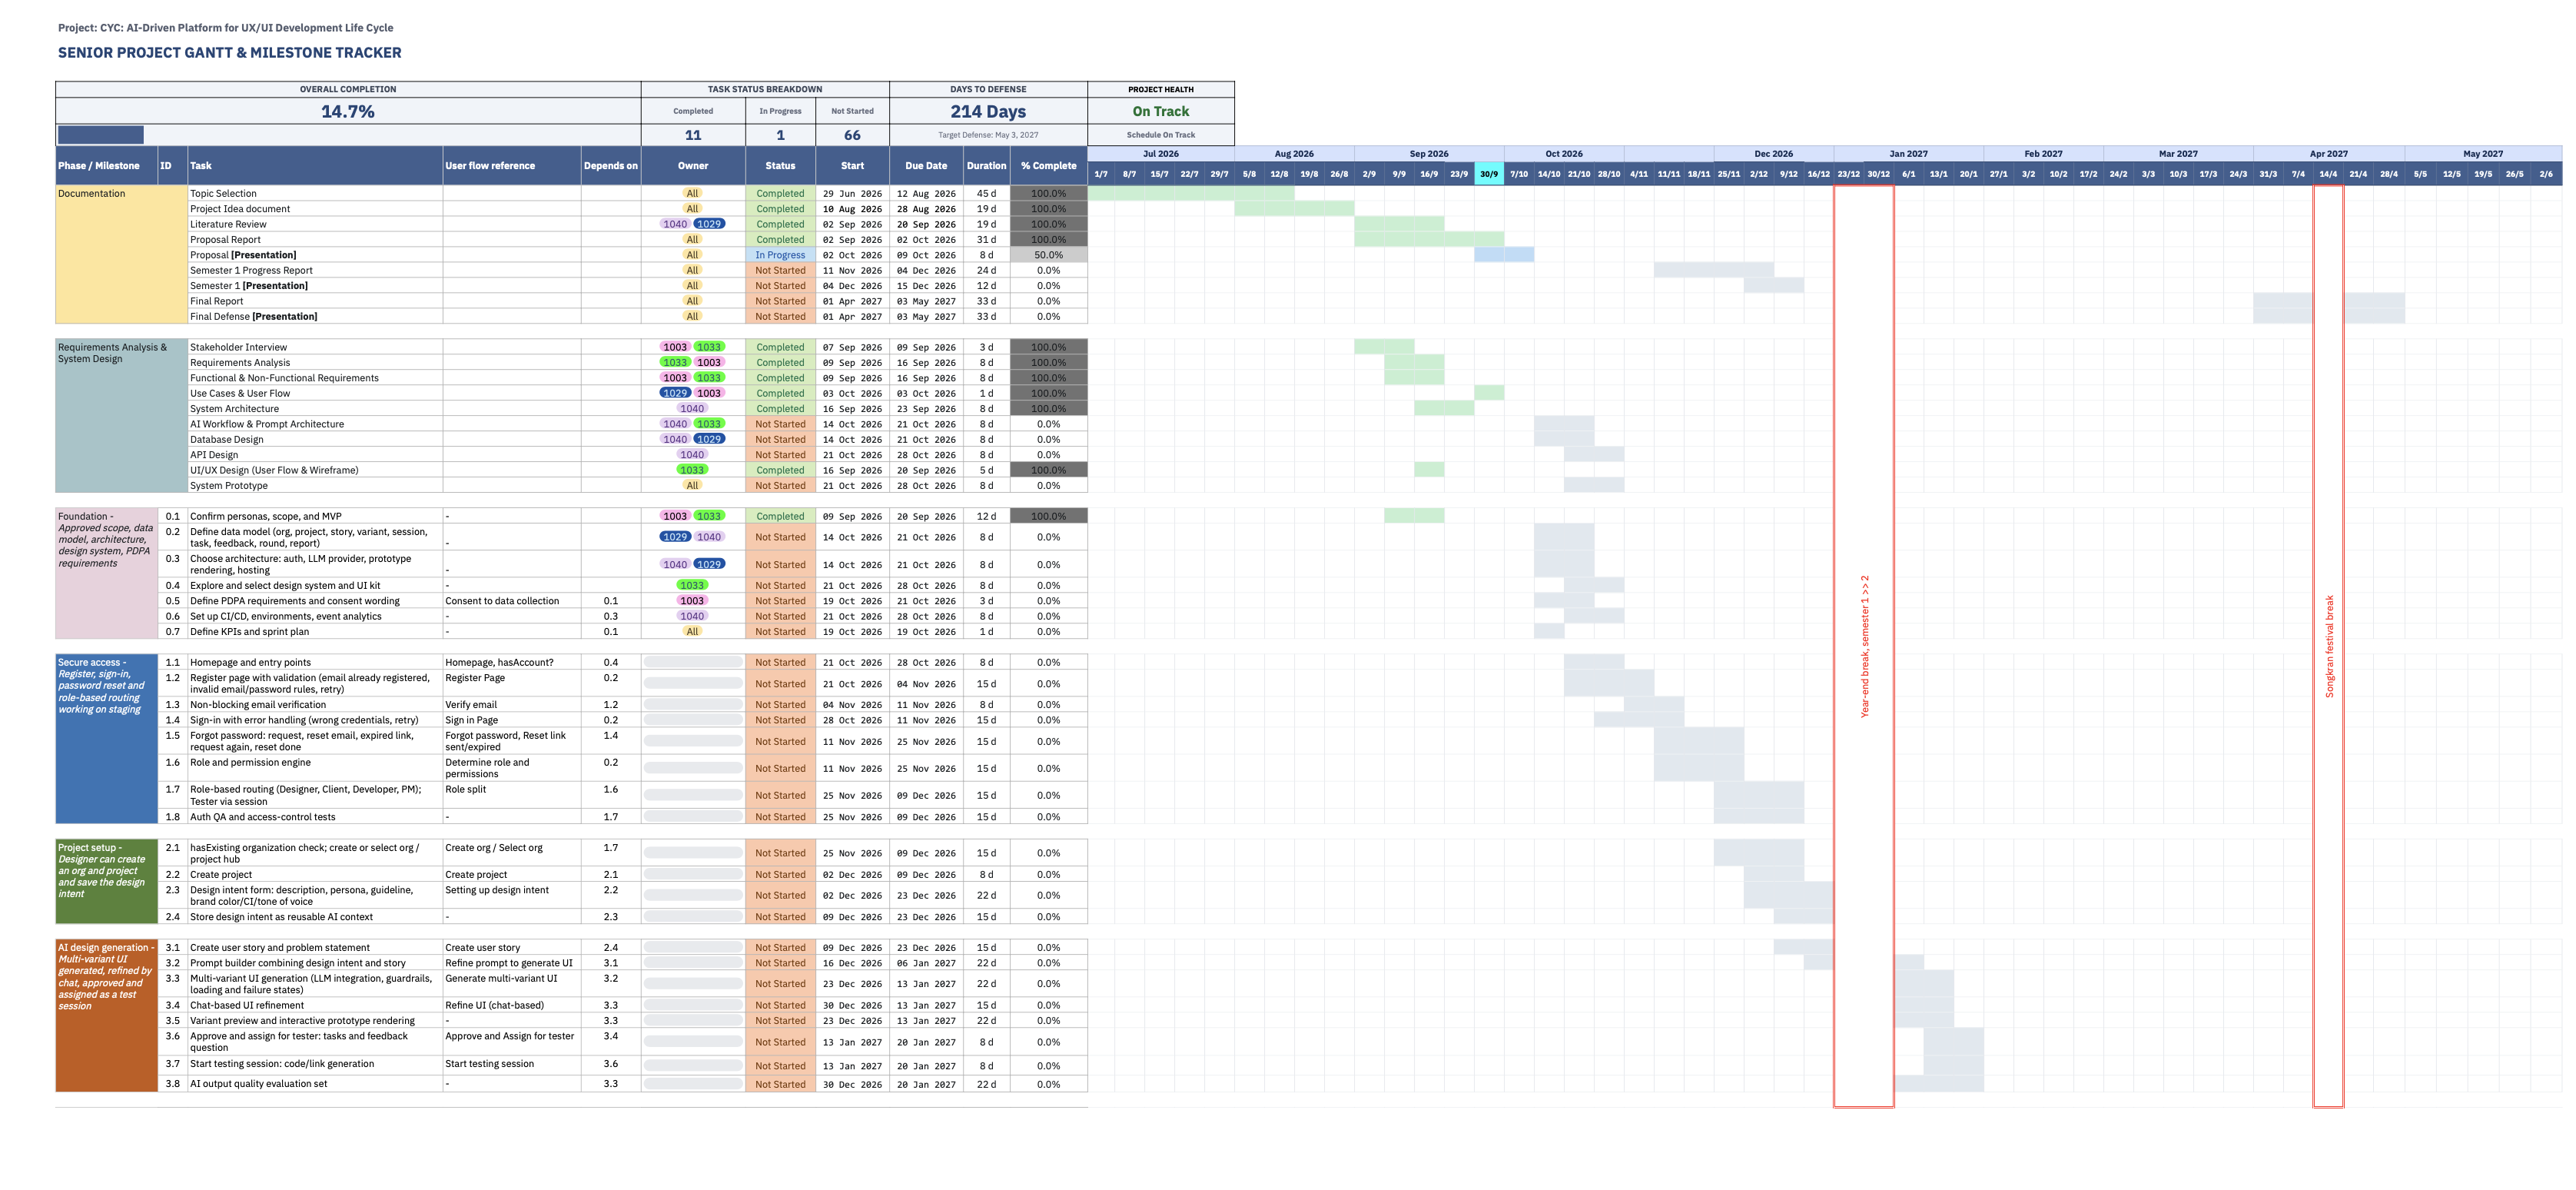
\includegraphics[
    width=0.9\textheight,
    height=0.95\linewidth,
    keepaspectratio,
    angle=90,
    origin=c
  ]{figures/ch1-introduction/gantt-sem1.png}
  \caption{Project Gantt chart สำหรับภาคการศึกษาที่ 1}
  \label{fig:gantt-semester-1}
\end{figure}

\clearpage

\begin{figure}[H]
  \centering
  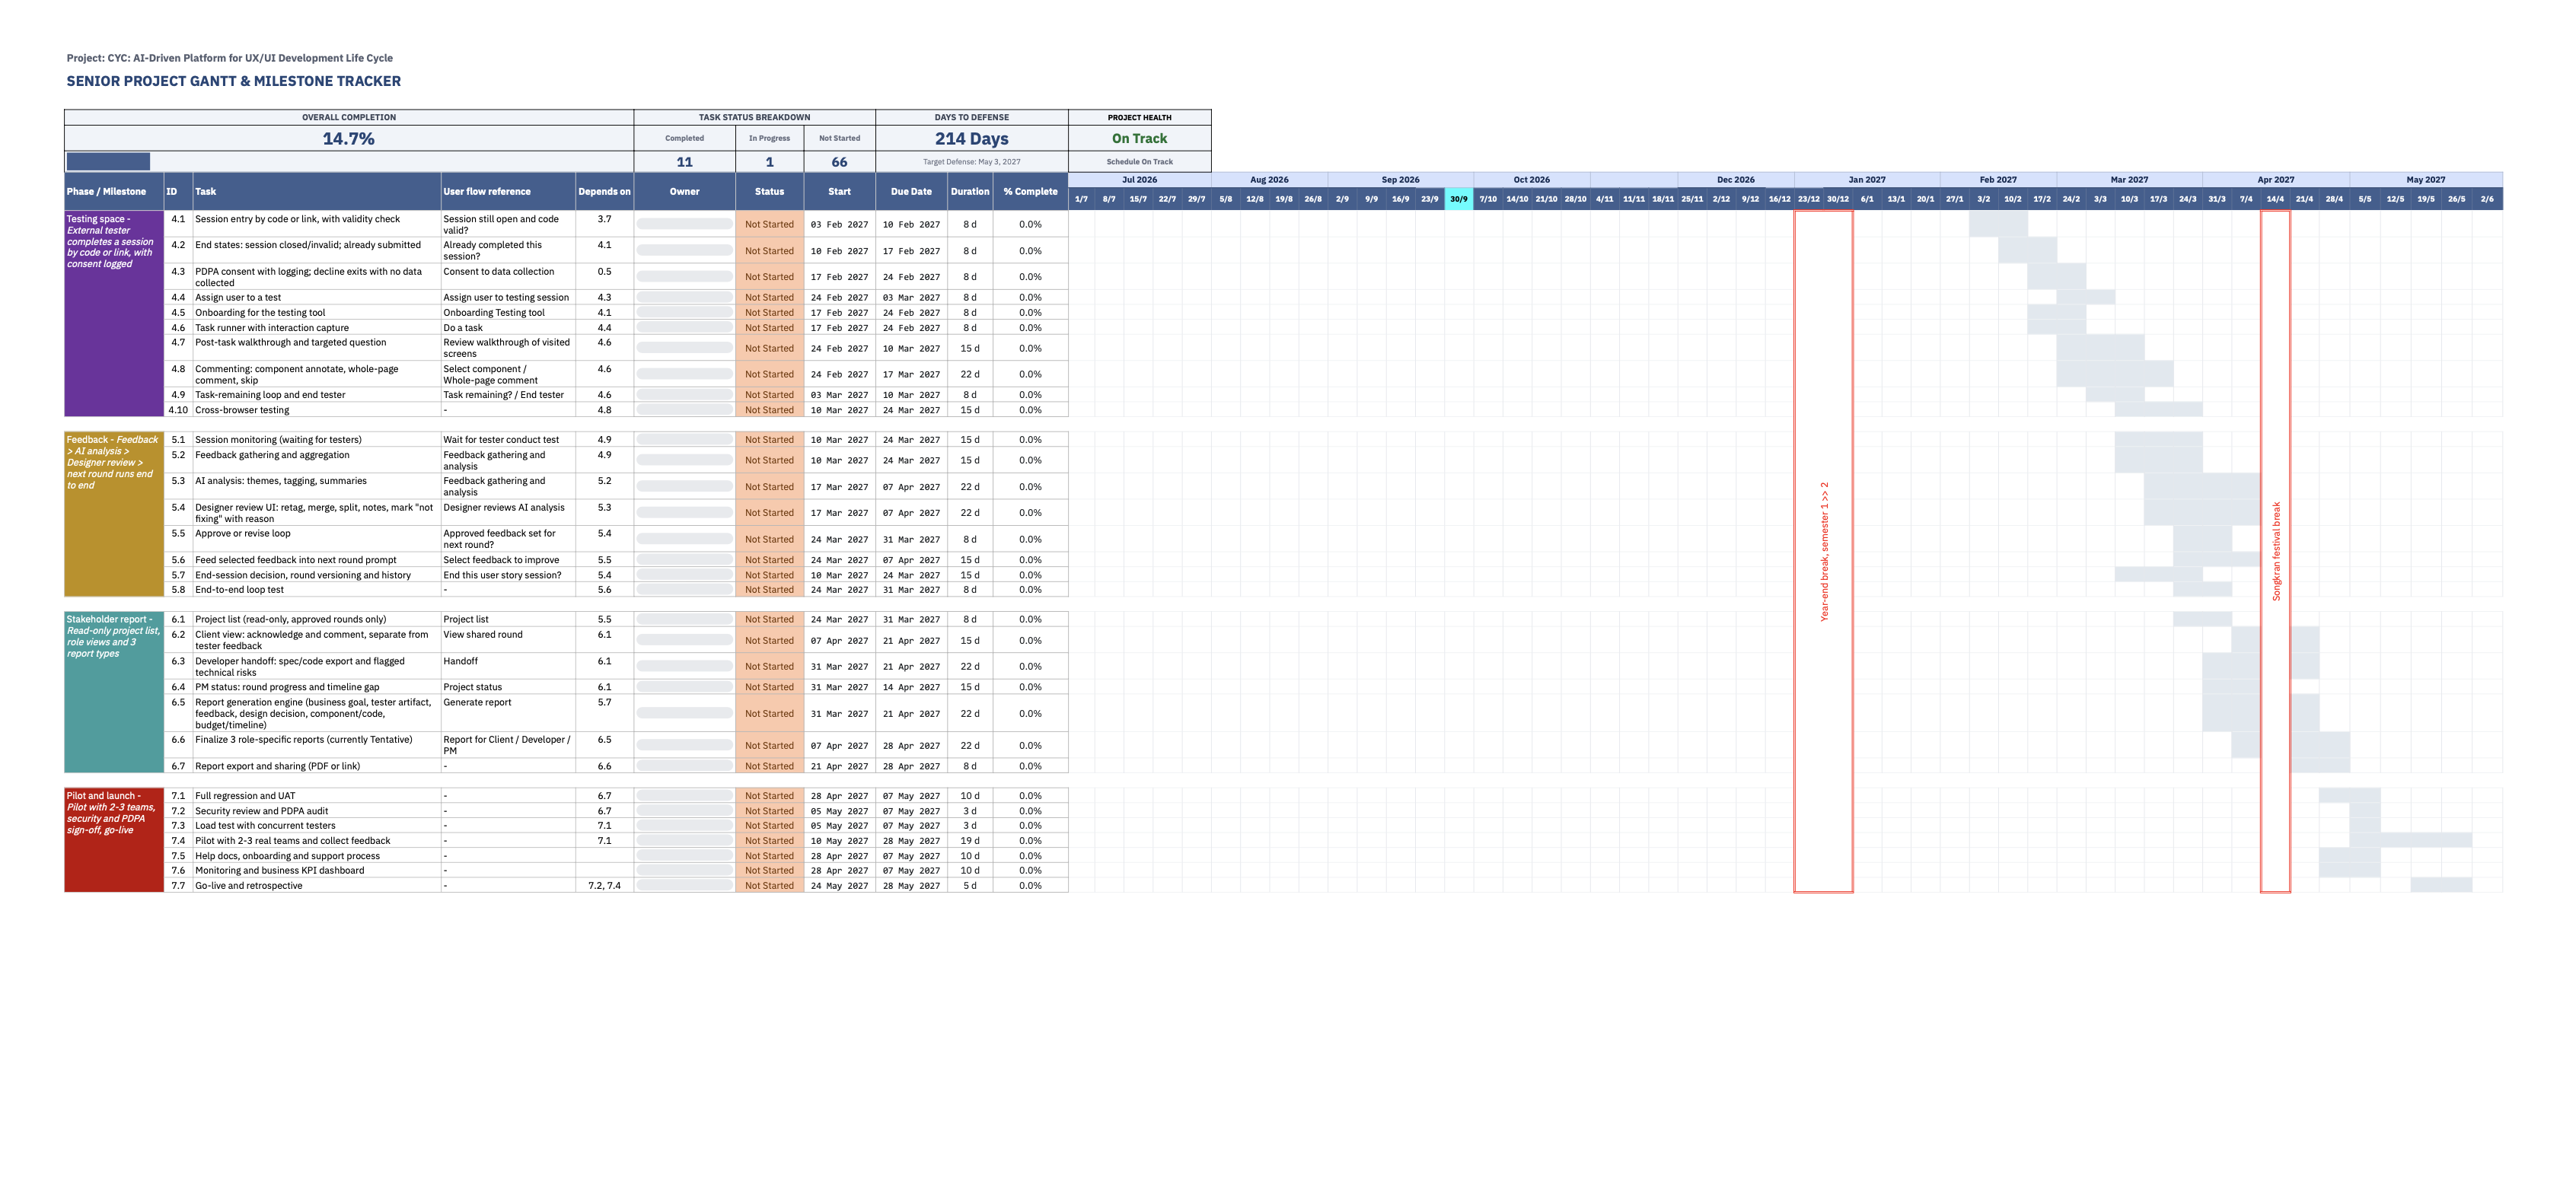
\includegraphics[
    width=0.9\textheight,
    height=0.95\linewidth,
    keepaspectratio,
    angle=90,
    origin=c
  ]{figures/ch1-introduction/gantt-sem2.png}
  \caption{Project Gantt chart สำหรับภาคการศึกษาที่ 2}
  \label{fig:gantt-semester-2}
\end{figure}
\subsection{สิ่งที่ส่งมอบ}
\subsubsection{ภาคการศึกษาที่ 1}
\begin{enumerate}
  \item \textbf{M0: Foundation}
    \begin{itemize}
      \item Software Requirement Specification, Data Model, System Architecture, Design System \& UI Kit, PDPA \& Consent, CI/CD, Sprint planning
    \end{itemize}
  \item \textbf{M1: Secure Access}
    \begin{itemize}
      \item ระบบสามารถสมัครสมาชิกพร้อมยืนยันอีเมล, เข้าสู่ระบบ ลืมและรีเซ็ตรหัสผ่าน ระบบสิทธิ์ตามบทบาท (Designer, Client, Developer, PM)
    \end{itemize}
  \item \textbf{M2: Project Setup}
    \begin{itemize}
      \item ระบบสามารถสร้าง organization และโปรเจกต์, แบบฟอร์มความต้องการทางการออกแบบ (description, persona, design guideline, CI, tone of voice)
    \end{itemize}
  \item \textbf{M3: AI Design Generation}
    \begin{itemize}
      \item ระบบสามารถสร้าง user story และ problem statement สร้าง two-alternative UI ด้วย Generative AI, Chat-based UI refinement, prototype preview อนุมัติและมอบหมายงานทดสอบ สร้าง test session (โดยสามารถเข้าถึงด้วยรหัสหรือลิงก์)
    \end{itemize}
\end{enumerate}

\subsubsection{ภาคการศึกษาที่ 2}
\begin{enumerate}
  \item \textbf{M4: Testing Space}
    \begin{itemize}
      \item ผู้เข้าร่วมทดสอบสามารถเข้า session ด้วยรหัสหรือลิงก์ ทำ task พร้อมให้ข้อเสนอแนะเชิงบริบท
    \end{itemize}
  \item \textbf{M5: Feedback}
    \begin{itemize}
      \item ระบบสามารถรวบรวมข้อเสนอแนะ AI สามารถวิเคราะห์รูปแบบ ข้อมูลเชิงลึกและประเด็นสำคัญ Designer ตรวจทานและแก้ไขผลการวิเคราะห์ เลือกข้อเสนอแนะที่จะปรับปรุงในรอบถัดไป บันทึกประวัติแต่ละรอบ
    \end{itemize}
  \item \textbf{M6: Stakeholder Report}
    \begin{itemize}
      \item ระบบสามารถแสดงหน้ารายการโปรเจกต์ (อ่านอย่างเดียว) มุมมองของ Client, Developer และ PM, รายงานสำหรับแต่ละบทบาท พร้อมส่งออก PDF หรือลิงก์
    \end{itemize}
  \item \textbf{M7: Pilot and Launch}
    \begin{itemize}
      \item ทดสอบระบบ (UAT, Load test, Security Test) ทดลองใช้กับ 2–3 ทีมตัวอย่าง, เอกสารการประกอบการใช้งาน เปิดใช้งานจริง
    \end{itemize}
\end{enumerate}


% !TeX root = ../../../proposal.tex
% Chapter 2: Related theory and works
\chapter{ทฤษฎีความรู้และงานที่เกี่ยวข้อง}
\thaijustify{
  ในบทที่ 2 นี้จะกล่าวถึงทฤษฎีที่เกี่ยวข้องที่ใช้ในการทำงานและการศึกษาเพื่อบรรลุวัตถุประสงค์ อธิบายคำศัพท์หรือภาษาทาง
  คอมพิวเตอร์ เทคโนโลยีที่จะนำมาประยุกต์ใช้งานและแก้ปัญหาต่าง ๆ ในโครงงาน รวมไปถึงงานวิจัย ผลิตภัณฑ์ หรือโครงงานที่นำมาใช้อ้างอิง เพื่อนำมาสังเคราะห์เป็นกรอบแนวคิดในการแก้ปัญหาและกำหนดขอบเขตของโครงงาน
}

\section{ทฤษฎีที่เกี่ยวข้อง}

\subsection{UX/UI Development Life Cycle: UX/UI DLC}
\thaijustify{
  กระบวนการออกแบบประสบการณ์ผู้ใช้และส่วนต่อประสานผู้ใช้เป็นกระบวนการที่เน้นผู้ใช้เป็นศูนย์กลางและต้องอาศัยการทำซ้ำอย่างต่อเนื่อง (Iterative process) โดยทั่วไปนักออกแบบจะต้องผ่านขั้นตอนตั้งแต่การรวบรวมความต้องการ การทำความเข้าใจผู้ใช้ (Empathize) การระบุปัญหา (Define) การระดมความคิด (Ideate) การสร้างต้นแบบ (Prototype) และการทดสอบ (Test)
}
\thaijustify{
  อย่างไรก็ตาม ในทางปฏิบัตินักออกแบบมักเผชิญข้อจำกัดด้านเวลาและทรัพยากร
  ทำให้การสำรวจแนวคิด การรับข้อเสนอแนะ และการปรับปรุงงานซ้ำหลายรอบทำได้ไม่เต็มที่
  Suh et al. \cite{suh2025storyensemble} ชี้ให้เห็นว่าข้อจำกัดดังกล่าวลดโอกาสในการสำรวจทางเลือกและย้อนกลับไปปรับแก้งานในขั้นตอนก่อนหน้า ขณะที่
  Feng et al. \cite{feng2023designing} แสดงให้เห็นว่าการสร้าง wireframe
  ด้วยมือเป็นงานที่ใช้เวลาและแรงงาน ซึ่งสามารถใช้ LLM ช่วยสร้าง wireframe
  จากความต้องการทางการออกแบบได้ และ Yuan et al. \cite{prototypeflow_humanai_ui_design} พบว่าการสร้าง
  UI ด้วย Generative AI ควรเปิดโอกาสให้นักออกแบบตรวจสอบและปรับผลลัพธ์ระหว่างกระบวนการ
  แทนการสร้างผลลัพธ์เพียงครั้งเดียว
}

\thaijustify{จากงานเหล่านี้จึงเห็นได้ว่า Generative AI สามารถช่วยลดภาระของงานที่ต้องทำ
  ด้วยมือและสนับสนุนกระบวนการออกแบบแบบวนซ้ำ ทำให้นักออกแบบมีเวลาสำหรับการทดสอบกับผู้ใช้และนำข้อเสนอแนะกลับมาปรับปรุงต้นแบบได้มากขึ้น
}

\subsection{ระเบียบวิธีการทดสอบการใช้งาน (Usability test)}
\thaijustify{
  การทดสอบกับผู้ใช้เป็นหัวใจสำคัญในการหาข้อบกพร่องและข้อควรปรับปรุงของงานออกแบบ
  โดยงานวิจัยชี้ให้เห็นว่าการทดสอบบ่อยครั้งกับกลุ่มตัวอย่างขนาดเล็กให้ข้อมูลเชิงลึกที่นำไปปรับปรุงได้จริงมากกว่าการทดสอบสเกลใหญ่แต่นาน ๆ ครั้ง โดย Nielsen \cite{nielsen2000five} เสนอว่า
  การทดสอบเชิงคุณภาพสามารถเริ่มต้นด้วยผู้เข้าร่วมประมาณ 5 คนต่อรอบ เนื่องจากภายใต้
  แบบจำลองการค้นพบปัญหาด้านการใช้งาน ผู้เข้าร่วม 5 คนสามารถค้นพบปัญหาได้ประมาณ
  ร้อยละ 85 และการเพิ่มผู้เข้าร่วมหลังจากนั้นมีแนวโน้มให้ข้อมูลใหม่ลดลงด้วย จึงควรนำผลที่ได้
  ไปปรับปรุงต้นแบบและทดสอบซ้ำในรอบถัดไป
  แนวคิดนี้สอดคล้องกับ Virzi \cite{virzi1992refining} ซึ่งพบว่าผู้เข้าร่วมประมาณ 4-5 คนสามารถค้นพบปัญหา
  ด้านการใช้งานได้ประมาณร้อยละ 80  และแบบจำลองของ
  Nielsen และ Landauer \cite{nielsen1993mathematical} ที่แสดงให้เห็นว่าประโยชน์จากการเพิ่มจำนวนผู้เข้าร่วมจะลดลง
  เรื่อย ๆ เมื่อปัญหาส่วนใหญ่ถูกค้นพบแล้ว อย่างไรก็ตาม จำนวนดังกล่าวเหมาะสำหรับการทดสอบเชิงคุณภาพเพื่อค้นหาปัญหาและปรับปรุงงานแบบวนซ้ำ ไม่ใช่เกณฑ์ตายตัวสำหรับการทดสอบทุกประเภท ใน UX/UI DLC มีระเบียบวิธีทดสอบการใช้งานที่นิยมใช้ ดังนี้
  \begin{itemize}
    \item \textbf{Usability Test} เป็นการทดสอบเพื่อให้ผู้เข้าร่วมทดสอบลองใช้งานระบบและหาจุดที่ใช้งานยากหรือติดขัด ซึ่งในขณะที่ทำการทดสอบผู้เข้าร่วมทดสอบจำเป็นต้องคิดไปด้วยพูดไปด้วย (Thinking-Aloud) โดยนักออกแบบจะคอยสังเกตพฤติกรรมและรับฟังความคิดเห็นของผู้เข้าร่วมทดสอบขณะทำภารกิจที่กำหนด \cite{rubin2008handbook, dumas1999practical, nielsen1993usability}
    \item \textbf{A/B Test} เป็นกระบวนการนำเสนอทางเลือกการออกแบบ (Variants) ที่แตกต่างกันให้กับผู้ใช้ เพื่อเปรียบเทียบประสิทธิภาพการใช้งานและรวบรวมข้อเสนอแนะก่อนที่จะตัดสินใจออกแบบในขั้นตอนถัดไป ในภาคอุตสาหกรรม A/B Test มักหมายถึงการทดลองแบบควบคุมบนระบบจริง (Online Controlled Experiment) ที่วัดผลด้วยสถิติโดยเมทริกซ์ต่าง ๆ เช่น conversion rate, click-throughs rate, task completion rate จากผู้ใช้จำนวนมาก \cite{kohavi2009controlled, kohavi2020trustworthy} อย่างไรก็ตาม วิธีนี้ให้ผลเป็นตัวเลขว่าทางเลือกใดทำงานได้ดีกว่า แต่ไม่อธิบายเหตุผลเบื้องหลังพฤติกรรมของผู้ใช้ จึงควรใช้ร่วมกับการรวบรวมข้อมูลเชิงคุณภาพ \cite{nielsen2005abtesting} % ในโครงงานนี้ A/B Test หมายถึงการให้ผู้ใช้กลุ่มเล็กลองใช้ต้นแบบสองรูปแบบและให้ข้อเสนอแนะในแต่ละรอบการทดสอบ ซึ่งเป็นแนวทางเชิงคุณภาพ
    \item \textbf{Comparative Usability Test} มีหลักการคล้าย A/B Test แต่เน้นการทดสอบเชิงคุณภาพและให้ผู้ใช้เปรียบเทียบดีไซน์ตั้งแต่สองรูปแบบขึ้นไปที่มีเป้าประสงค์เดียวกัน งานวิจัยพบว่าการให้ผู้ใช้เห็นทางเลือกการออกแบบหลายแบบพร้อมกันช่วยให้ผู้ใช้ให้ความคิดเห็นได้เปิดกว้างและลึกกว่าการทดสอบการใช้งานจากดีไซน์แบบเดียว~\cite{tohidi2006getting} อีกทั้งการสร้างต้นแบบหลายแบบยังนำไปสู่ผลงานที่ดีขึ้นและมีความหลากหลายของแนวคิดมากขึ้น~\cite{dow2010parallel}
  \end{itemize}
  จากการศึกษาข้างต้น โครงงานนี้เลือกใช้ \textit{Comparative Usability Test}
  เป็นหลัก โดยให้ผู้เข้าร่วมทดสอบเปรียบเทียบ two-alternative UI และให้ข้อเสนอแนะในแต่ละรูปแบบ เนื่องจากโครงงานนี้มุ่งเน้นการค้นหาปัญหาและความต้องการของผู้ใช้จากต้นแบบ เพื่อนำข้อเสนอแนะที่ได้กลับไปปรับปรุงการออกแบบในรอบถัดไป
  ทั้งนี้ Generative AI จะถูกนำมาใช้เพื่อช่วยสร้าง two-alternative UI รวบรวม
  และวิเคราะห์ข้อเสนอแนะ เพื่อลดภาระงานของนักออกแบบในการทดสอบแต่ละรอบ
}

\subsection{การสกัดความต้องการและการสร้าง User Persona จากข้อเสนอแนะของผู้ใช้}
\thaijustify{
  การทำความเข้าใจความต้องการของผู้ใช้เป็นส่วนสำคัญของกระบวนการออกแบบ
  โดยการใช้ต้นแบบเป็นหนึ่งในวิธีที่ช่วยให้นักออกแบบสามารถสกัดความต้องการ
  และรับข้อเสนอแนะจากผู้ใช้ได้ก่อนการพัฒนาระบบจริง \cite{pacheco2018}
  UI prototype  ยังใช้ทดสอบ ประเมิน และยืนยันแนวคิดร่วมกับผู้ใช้และทีมพัฒนาได้~\cite{kolthoff2024}โครงงานนี้เลือกใช้ต้นแบบระดับ high-fidelity เพื่อให้ผู้เข้าร่วมทดสอบสามารถชี้ข้อเสนอแนะไปยัง component ที่ต้องการได้โดยตรง ข้อมูลที่ได้จากการทดสอบต้นแบบจึงสามารถนำมาใช้เพื่อค้นหาปัญหาการใช้งาน ความต้องการ และความแตกต่างระหว่างผู้ใช้แต่ละกลุ่มได้
 
}
\thaijustify{
  อย่างไรก็ตาม ข้อเสนอแนะจากผู้ใช้ไม่ควรถูกตีความว่าเป็นปัญหาการใช้งาน
  หรือความต้องการโดยตรงทั้งหมด เนื่องจากความชอบของผู้ใช้อาจไม่สอดคล้อง
  กับประสิทธิภาพการใช้งานเสมอไป \cite{nngroup_satisfaction} และการใช้ผลการโหวตจากผู้เข้าร่วมจำนวนไม่มากเป็นข้อมูลเชิงปริมาณ อาจทำให้เกิดความเข้าใจผิดได้ \cite{nngroup_qualitative} นอกจากนี้ ข้อเสนอแนะจากผู้มีส่วนได้ส่วนเสียในแต่ละกลุ่มอาจมีความสำคัญแตกต่างกันตามบทบาท ความต้องการ ความเร่งด่วน และอิทธิพลต่อโครงการ \cite{shukla2025,mitchell1997} ดังนั้น การวิเคราะห์ข้อเสนอแนะจึงควรพิจารณาทั้งเนื้อหาของข้อเสนอแนะและบริบทของกลุ่มผู้ให้ข้อเสนอแนะร่วมกัน
}
\thaijustify{
  วิธีหนึ่งในการนำข้อมูลดังกล่าวมาใช้สนับสนุนกระบวนการออกแบบคือ
  User Persona ซึ่งเป็นตัวแทนของกลุ่มผู้ใช้ที่สร้างขึ้นจากข้อมูลของผู้ใช้
  เพื่อสรุปลักษณะและความต้องการที่สำคัญของแต่ละกลุ่ม งานของ
  Shin et al. \cite{shin2024} ศึกษาการใช้ Large Language Models
  ร่วมกับมนุษย์ในการสร้าง Persona จากข้อมูลผู้ใช้ ซึ่งพบว่าการให้ LLM
  สร้าง Persona จากข้อมูลทั้งหมดโดยอัตโนมัติยังมีข้อจำกัดในการระบุลักษณะสำคัญของกลุ่มผู้ใช้ ในทางกลับกัน การให้มนุษย์มีส่วนร่วมในการ
  ระบุและจัดกลุ่มข้อมูลตามลักษณะที่สำคัญ แล้วใช้ LLM ช่วยสรุปข้อมูลของแต่ละกลุ่มเป็น Persona สามารถสร้าง Persona ที่เป็นตัวแทนของข้อมูลผู้ใช้ได้ดีกว่า แนวทางดังกล่าวจึงสนับสนุนแนวคิด Human-in-the-loop
  แทนการให้ Generative AI เป็นผู้กำหนด Persona เพียงอย่างเดียว
}
\thaijustify{
  จากแนวคิดดังกล่าว โครงงานนี้จึงนำข้อเสนอแนะที่ได้จาก Comparative Usability Test มาใช้เป็นข้อมูลเชิงคุณภาพ โดยแยกพิจารณาปัญหาการใช้งาน ความชอบ และกลุ่มของผู้ให้ข้อเสนอแนะ จากนั้นใช้ Generative AI ช่วยรวบรวมและสรุปลักษณะร่วมของข้อมูลเพื่อสนับสนุนการสร้าง User Persona โดยให้นักออกแบบเป็นผู้ตรวจสอบและยืนยันการจัดกลุ่มและผลลัพธ์ที่ได้ Persona ที่ผ่านการตรวจสอบแล้วจึงสามารถใช้เป็นตัวแทนของความต้องการของผู้ใช้แต่ละกลุ่ม และเป็นข้อมูลประกอบการตัดสินใจในการปรับปรุง two-alternative UI ในรอบการออกแบบถัดไปได้
}

\subsection{ข้อกำหนดระบบการออกแบบด้วย Generative AI}
\thaijustify{
  การทำงานกับ Generative AI เพื่อสร้าง two-alternative UI จำเป็นต้องมีกรอบควบคุม (Guardrails) เพื่อให้ผลลัพธ์ที่ได้สอดคล้องกับอัตลักษณ์ของผู้ว่าจ้างหรือผลิตภัณฑ์นั้น ๆ Figma \cite{figma_agent} ระบุว่าการใช้ Design System ช่วยเป็นกรอบให้ Generative AI สามารถสร้างทางเลือกการออกแบบที่ถูกต้องได้ และ Design Tokens Community Group \cite{designtokens2025} ได้กำหนดมาตรฐานรูปแบบไฟล์สำหรับการแลกเปลี่ยน Design tokens ระหว่างเครื่องมือไว้ โครงงานนี้จึงกำหนดให้ Design System เป็นข้อบังคับใช้ควบคุมในการสร้าง UI ด้วย Generative AI และใช้ตรวจสอบความถูกต้องก่อนการส่งมอบ
}
% /2.1.6 - 2.2.3 เอามารวมกันเลย
\section{โครงงาน งานวิจัยหรือผลิตภัณฑ์ที่เกี่ยวข้อง}

\subsection{การสร้าง UI และวิเคราะห์ข้อเสนอแนะด้วย Generative AI}

\thaijustify{
  งานวิจัยด้านการสร้าง UI ด้วย LLM แสดงให้เห็นทั้งศักยภาพและข้อจำกัดของเทคโนโลยี โดย Kolthoff et al. \cite{kolthoff2024} พบว่าการสร้าง UI ยังมีข้อผิดพลาดด้านการจัดวาง การตีความฟังก์ชัน และความไม่สอดคล้องขององค์ประกอบ เช่น สี ตัวอักษร และรูปแบบของ component ขณะที่ Ataei et al. \cite{ataei2025} ใช้ LLM Agents จำลองผู้ใช้เพื่อค้นหาความต้องการที่ไม่ได้ถูกระบุโดยตรง แต่ยังไม่ได้มุ่งเน้นการทดสอบต้นแบบกับผู้เข้าร่วมทดสอบแบบวนซ้ำ ส่วน Suh et al. \cite{suh2024} เสนอการใช้ LLM เพื่อสร้างและสำรวจทางเลือกหลายรูปแบบ แต่ยังไม่ได้เชื่อมทางเลือกเหล่านั้นเข้ากับการทดสอบการใช้งานและข้อเสนอแนะจากผู้เข้าร่วมทดสอบ
}

\thaijustify{
  อย่างไรก็ตาม LLM ยังมีอคติในการตัดสินใจ เช่น มีแนวโน้มตอบปฏิเสธมากเกินไปในงานที่ต้องตัดสินใจแบบใช่หรือไม่ใช่ โดยเฉพาะเมื่อโมเดลมีความรู้ไม่เพียงพอ ขณะที่การให้บริบทที่เกี่ยวข้องและการเปิดตัวเลือก ''ไม่ทราบ'' ช่วยลดอคตินี้ได้~\cite{song2025} ประเด็นนี้ต้องคำนึงถึงเมื่อให้ LLM จำแนกข้อเสนอแนะแบบเลือกตอบ เช่น การตัดสินว่าข้อเสนอแนะหนึ่งเป็นปัญหาการใช้งานหรือไม่ นอกจากนี้ การสร้าง Persona จากข้อมูลผู้ใช้ยังต้องอาศัยมนุษย์ช่วยระบุและตรวจสอบลักษณะที่สำคัญของแต่ละกลุ่ม~\cite{shin2024}
  \cite{shin2024}
}

\thaijustify{
  จากข้อจำกัดดังกล่าว โครงงานนี้จึงนำ Generative AI มาใช้สนับสนุน
  กระบวนการแบบวนซ้ำตั้งแต่การสร้าง two-alternative UI การทดสอบกับผู้ใช้จริง การรวบรวมและวิเคราะห์ข้อเสนอแนะ ไปจนถึงการสังเคราะห์ข้อมูลสำหรับ Persona Artifact โดยให้นักออกแบบตรวจสอบและยืนยันผลการวิเคราะห์
  ก่อนเลือกข้อมูลที่จะนำไปใช้ปรับปรุงและสร้าง two-alternative UI สำหรับการทดสอบในรอบถัดไป
}

\subsection{แนวทางการปฏิสัมพันธ์ระหว่างมนุษย์กับปัญญาประดิษฐ์}
\thaijustify{
  Pourasad \& Maalej \cite{pourasad2025} ศึกษาการใช้ LLM เพื่อค้นหาปัญหาด้านการใช้งานของแอปพลิเคชัน และพบว่าปัญญาประดิษฐ์สามารถระบุปัญหาที่ถูกต้องได้บางส่วนแต่ยังพลาดปัญหาส่วนใหญ่ที่พบจากการทดสอบกับผู้ใช้ เนื่องจากปัญญาประดิษฐ์ วิเคราะห์จากข้อมูลของระบบและหน้าจอ แต่ไม่สามารถสะท้อนพฤติกรรม ความเข้าใจและปัญหาที่เกิดขึ้นระหว่างการใช้งานจริงของผู้ใช้ได้ทั้งหมด ดังนั้น ปัญญาประดิษฐ์จึงเหมาะกับการใช้เป็นเครื่องมือช่วยวิเคราะห์มากกว่าการทดแทนการทดสอบกับผู้ใช้จริง
}
\thaijustify{
  แนวคิดนี้สอดคล้องกับ Amershi et al. \cite{amershi2019} ที่เสนอให้ระบบปัญญาประดิษฐ์เปิดเผยความสามารถและข้อจำกัด รวมถึงเปิดโอกาสให้ผู้ใช้แก้ไขผลลัพธ์เมื่อปัญญาประดิษฐ์ทำงานผิดพลาด โครงงานนี้จึงให้ผู้ใช้จริงเป็นผู้ทดสอบและให้ข้อเสนอแนะ ส่วนปัญญาประดิษฐ์ทำหน้าที่ช่วยรวบรวม วิเคราะห์ และสรุปข้อมูล โดยให้นักออกแบบเป็นผู้ตรวจสอบและตัดสินใจขั้นสุดท้ายก่อนนำผลไปใช้ในรอบการออกแบบถัดไป
}

\subsection{ผลิตภัณฑ์และเครื่องมือในตลาดปัจจุบัน}
\thaijustify{
  จากการสำรวจผลิตภัณฑ์ที่เกี่ยวข้อง ณ ปัจจุบัน พบว่าเครื่องมือแต่ละกลุ่มมีจุดเด่นและข้อจำกัดที่ต่างกัน ได้แก่
  \begin{itemize}
    \item \textbf{เครื่องมือ A/B Testing (เช่น Kameleoon, Otter)} มักทำงานกับเว็บไซต์ที่พัฒนาเสร็จแล้ว (Live site) เพื่อวัดพฤติกรรมผู้ใช้ ซึ่งต่างจากโครงงานนี้ที่ทำงานกับต้นแบบก่อนการพัฒนา \cite{kameleoon, otterab}
      \begin{figure}[H]
        \centering
        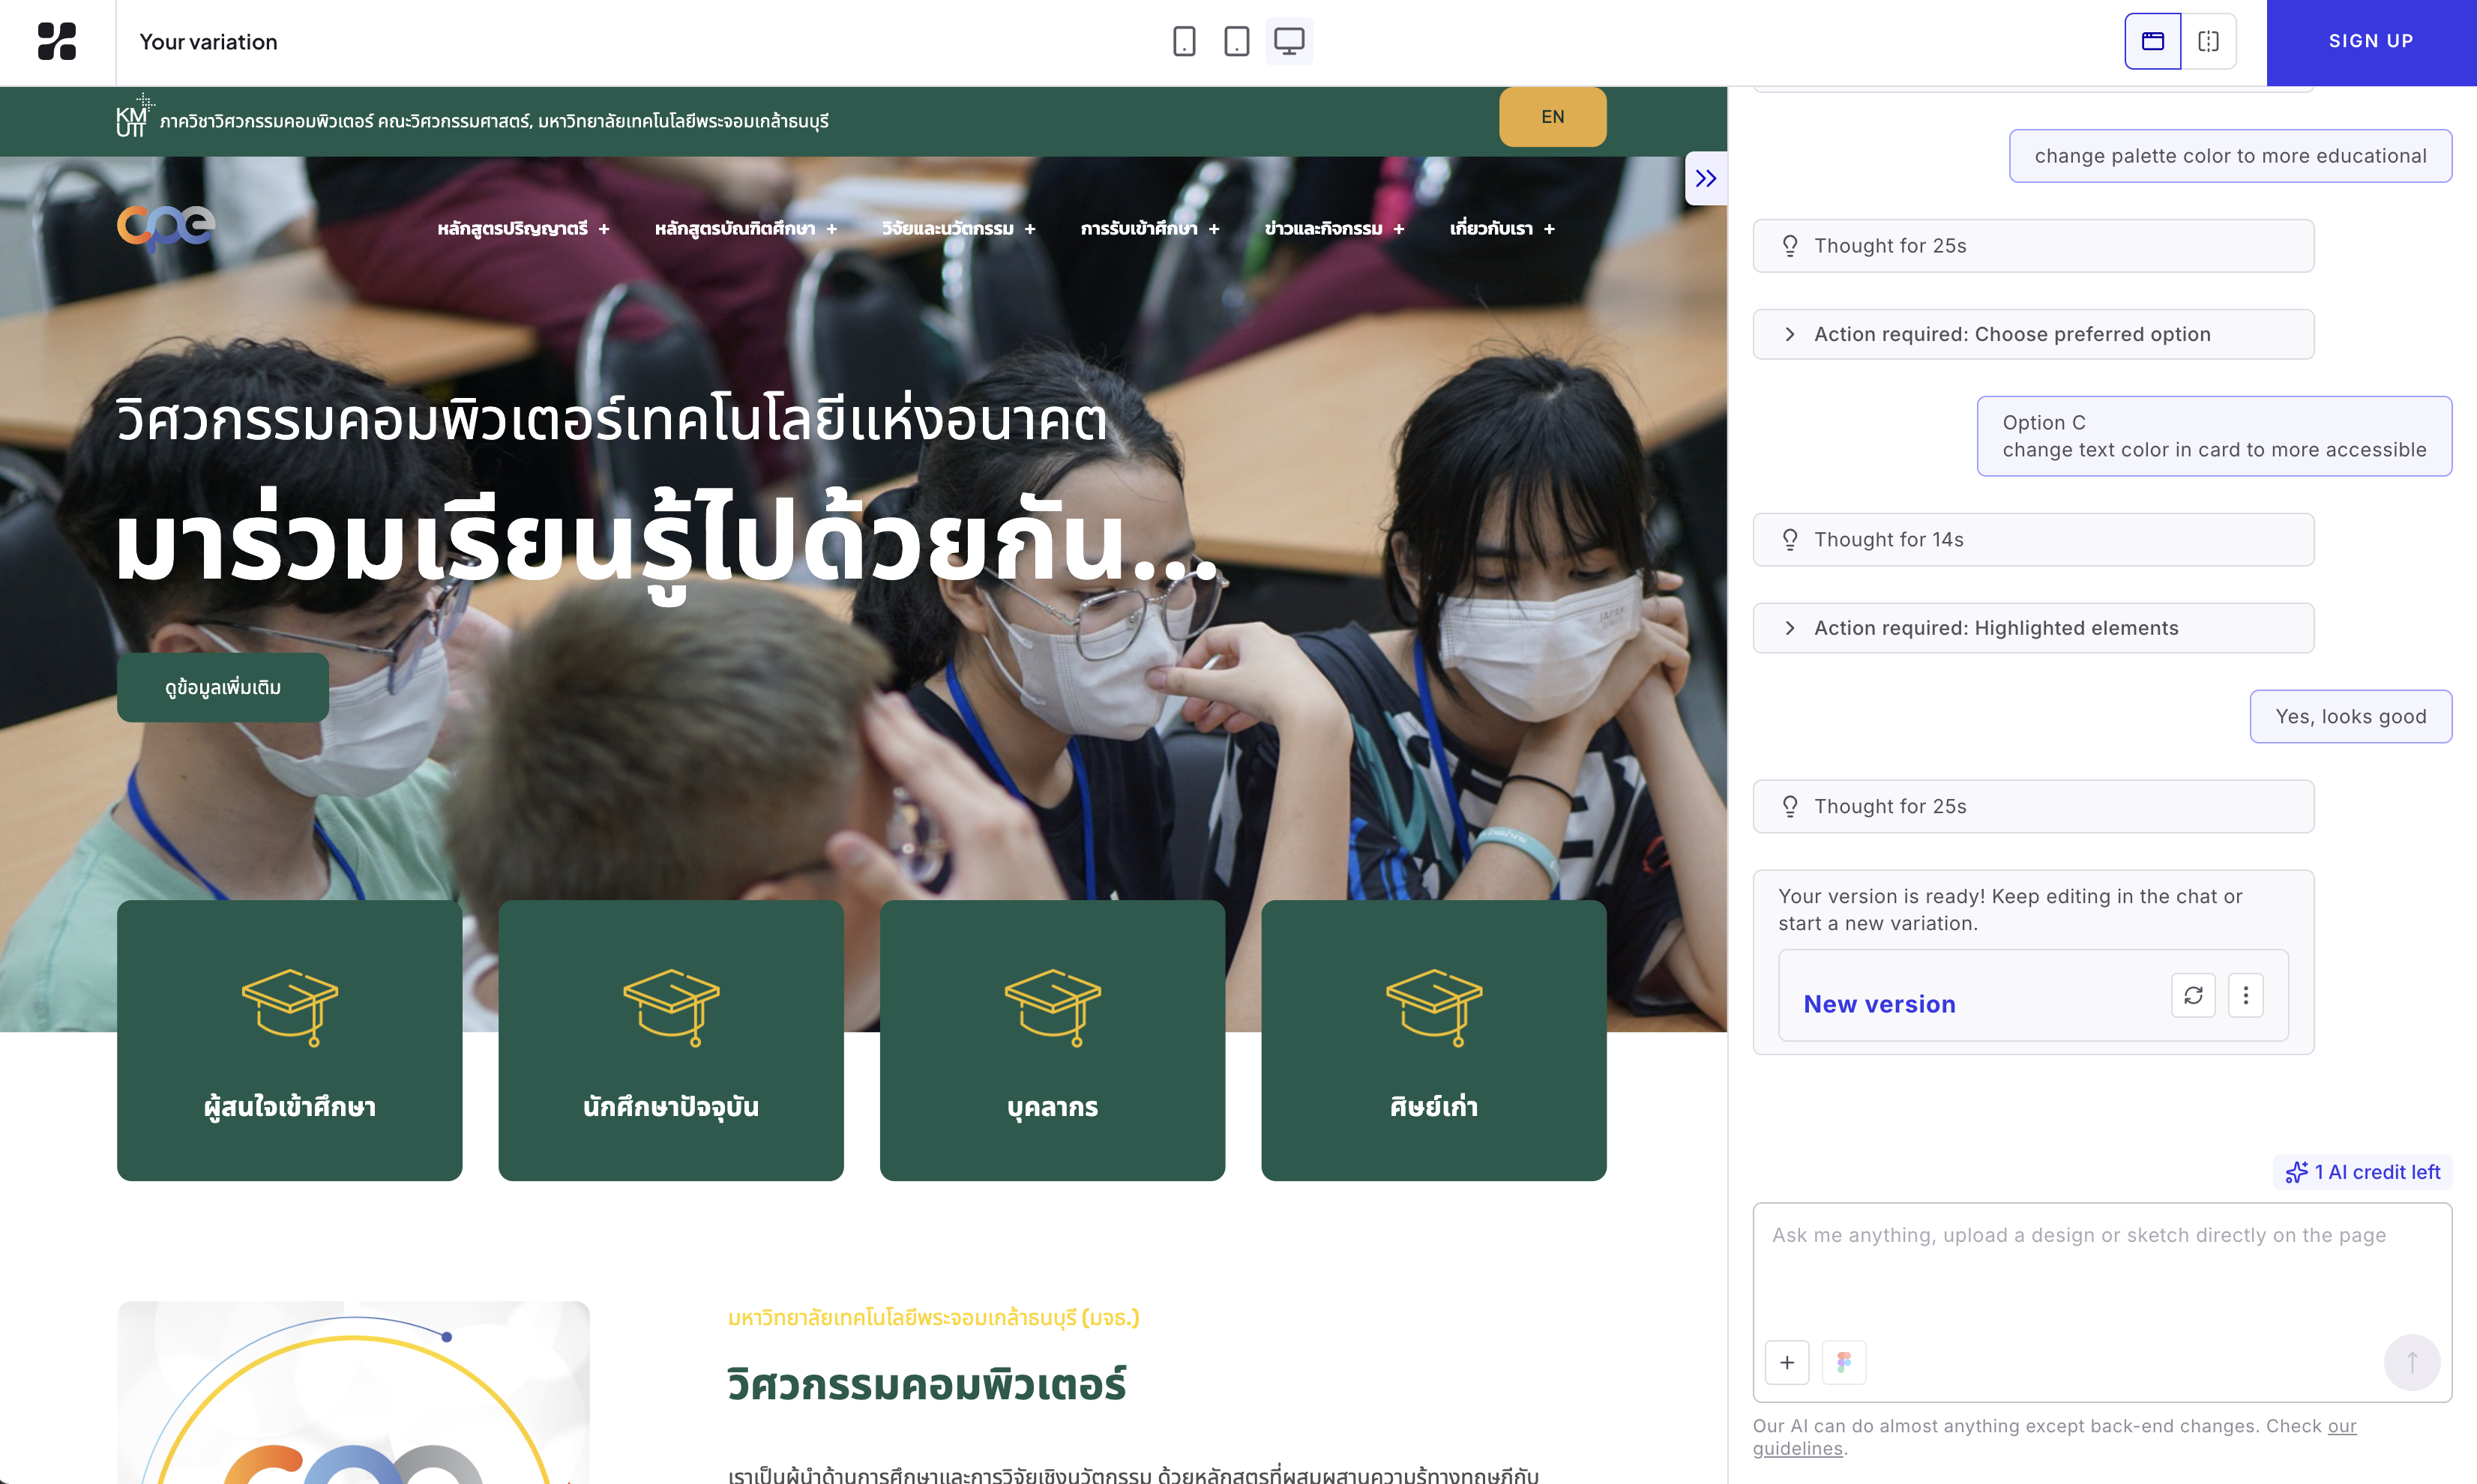
\includegraphics[
          width=0.5\textheight,
          height=0.95\linewidth,
          keepaspectratio,
          origin=c
        ]{figures/ch2-literature-review/kameleoon.png}
        \caption{แพลตฟอร์ม Kameleoon ใช้สำหรับการทำ A/B Testing}
        \label{fig:kameleoon}
      \end{figure}

    \item \textbf{เครื่องมือทดสอบผู้ใช้ก่อนเขียนโค้ด (เช่น Lyssna, Useberry)} มีฟังก์ชัน Preference testing สำหรับเปรียบเทียบดีไซน์หลายแบบ~\cite{lyssna,useberry} และ Lyssna เริ่มมี AI ช่วยสรุปธีมหลักจากคำตอบของผู้เข้าร่วมแล้ว~\cite{lyssna_synthesize} แต่จากการสำรวจเครื่องมือกลุ่มนี้ยังไม่ใช้ AI สร้างทางเลือกการออกแบบ (Variants) และยังไม่แยกปัญหาการใช้งาน (Pain point) ออกจากความชอบของผู้ใช้ในระบบเดียวกัน
      \begin{figure}[H]
        \centering
        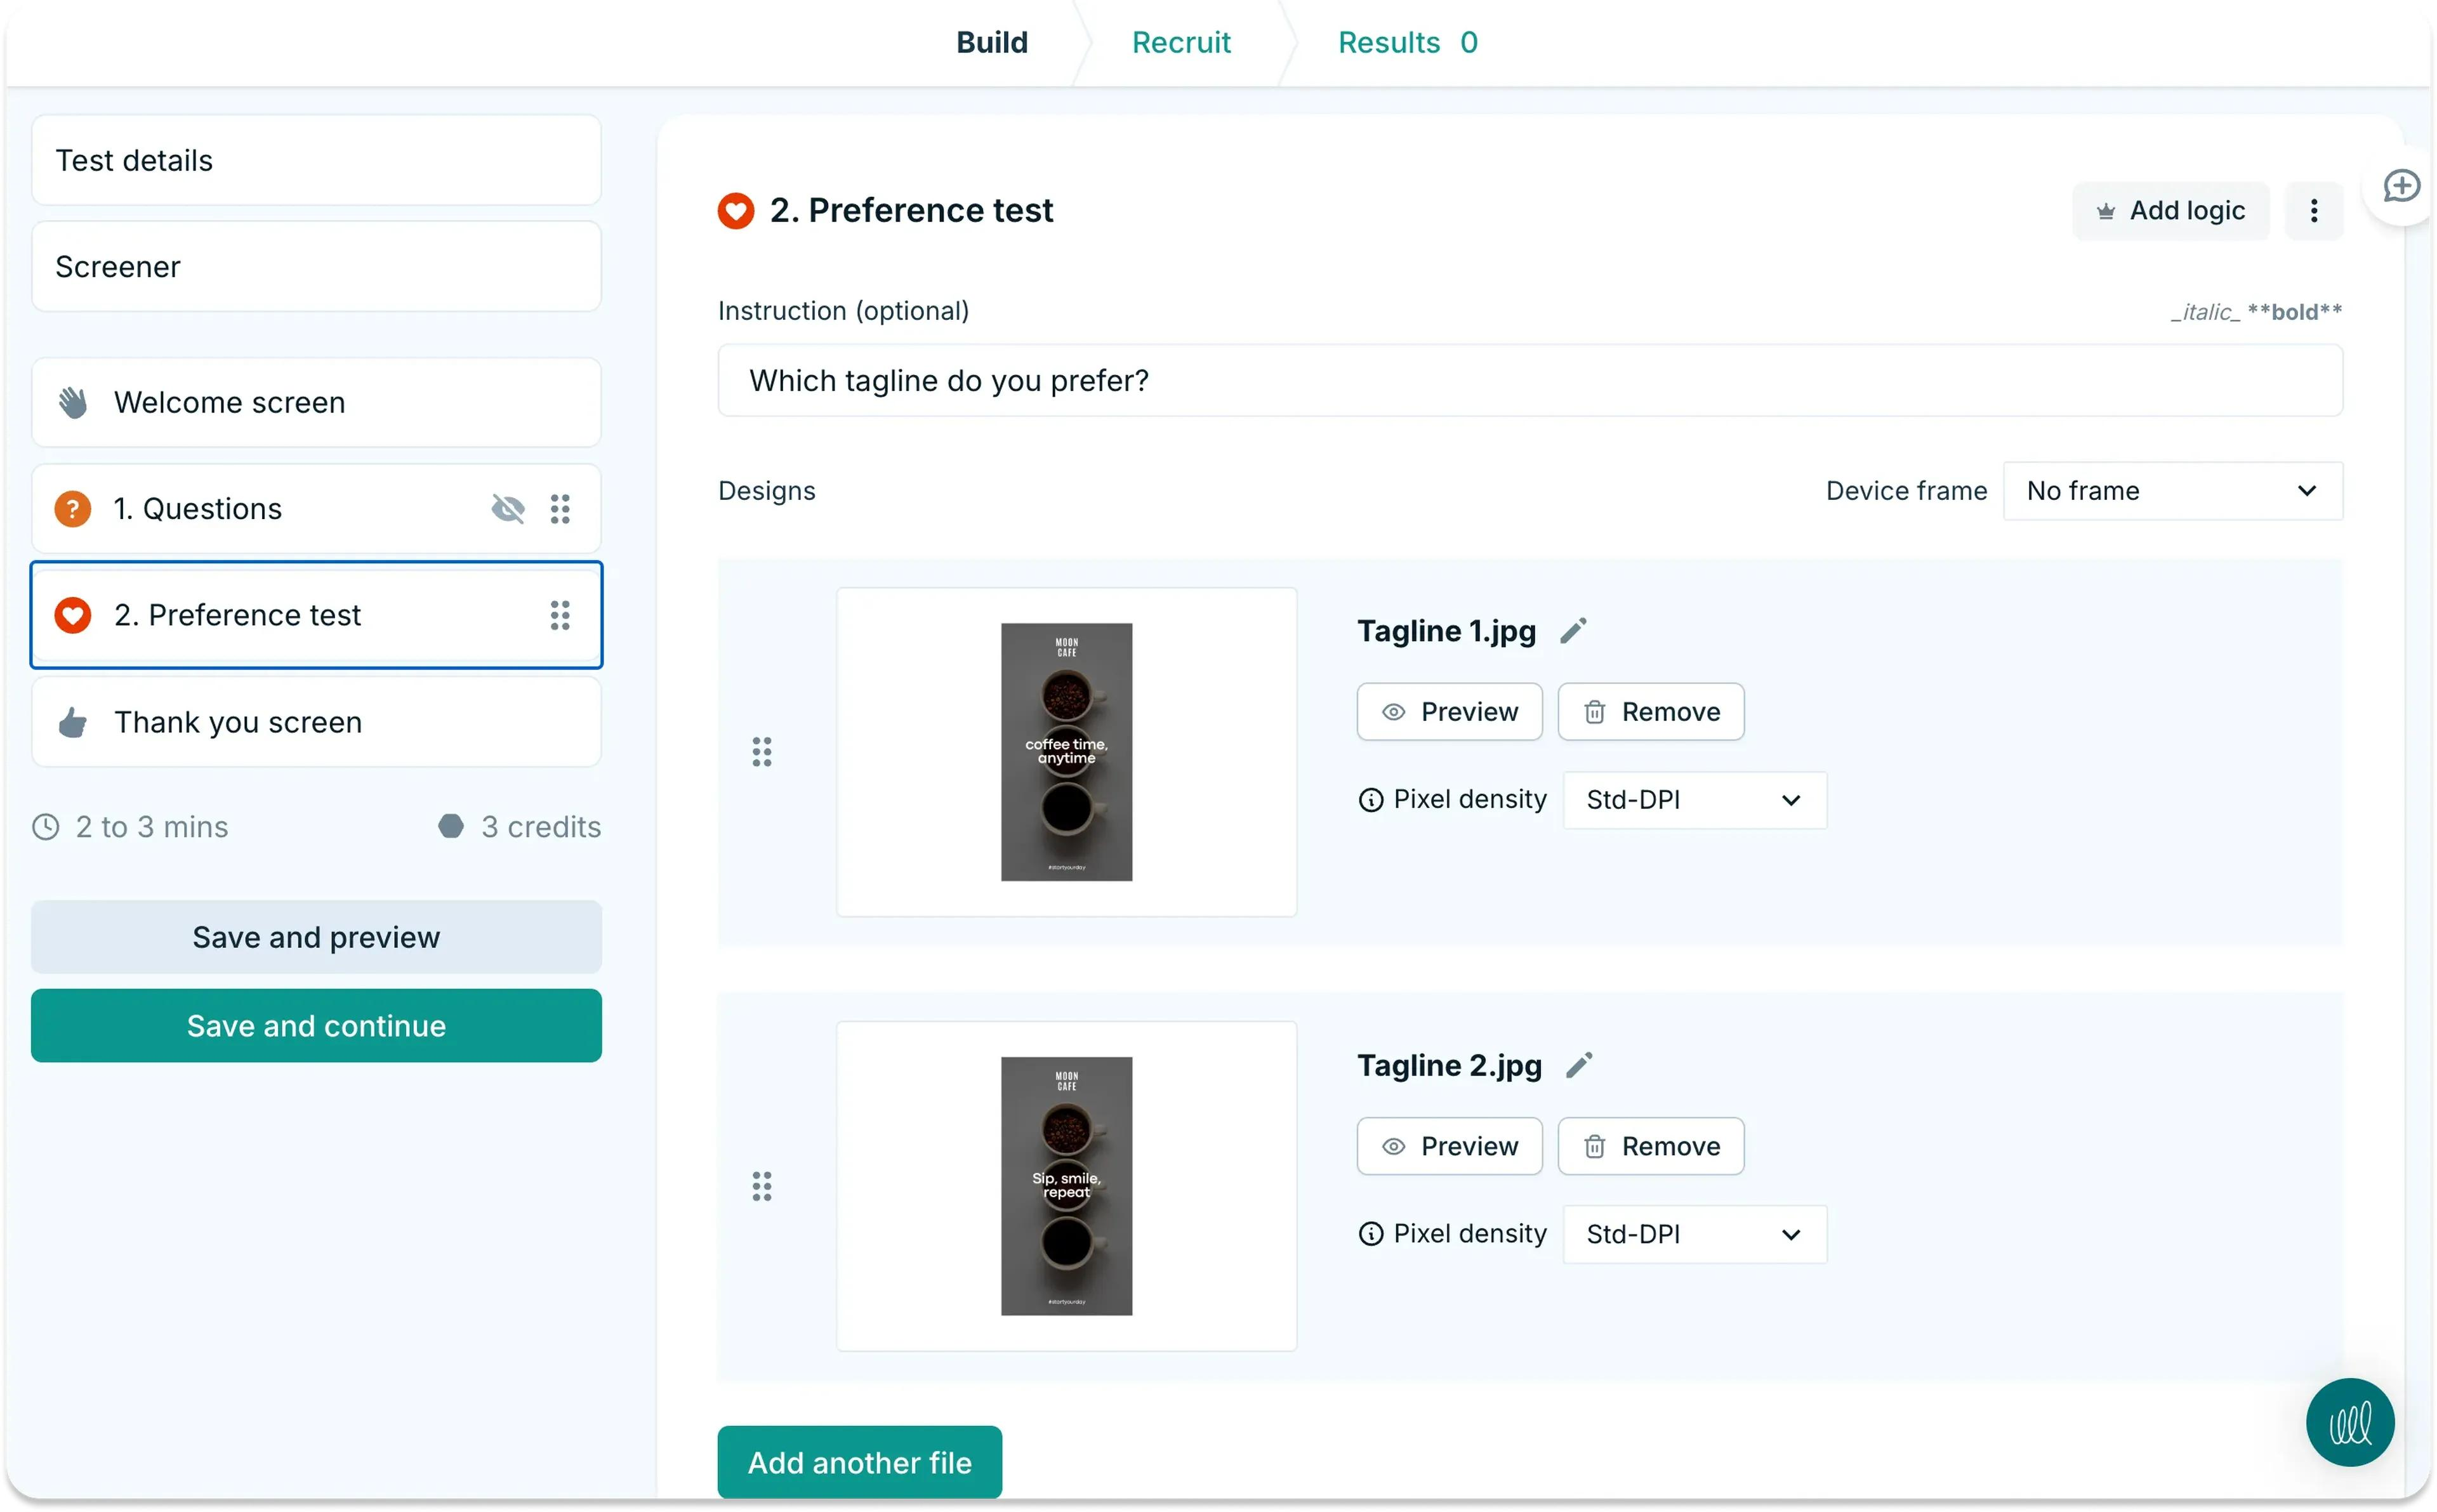
\includegraphics[
          width=0.5\textheight,
          height=0.95\linewidth,
          keepaspectratio,
          origin=c
        ]{figures/ch2-literature-review/lyssna.png}
        \caption{แพลตฟอร์ม Lyssna ใช้สำหรับการทดสอบการใช้งาน}
        \label{fig:lyssna}
      \end{figure}

    \item \textbf{เครื่องมือออกแบบที่มีปัญญาประดิษฐ์เป็นตัวช่วยในการทำงาน (เช่น Figma Make, Figma Agent)} สามารถสร้างต้นแบบหรือ Variants จากคำสั่งได้ โดย agent ของ Figma สร้าง Variants สำหรับ split test จาก component, token และ style ของ Design System~\cite{figma_agent} อย่างไรก็ตาม จากการสำรวจเครื่องมือกลุ่มนี้ยังไม่มีระบบรวบรวมข้อเสนอแนะจากผู้ทดสอบหลายกลุ่มเพื่อนำมาวิเคราะห์ร่วมกัน\cite{figma_agent}
      \begin{figure}[H]
        \centering
        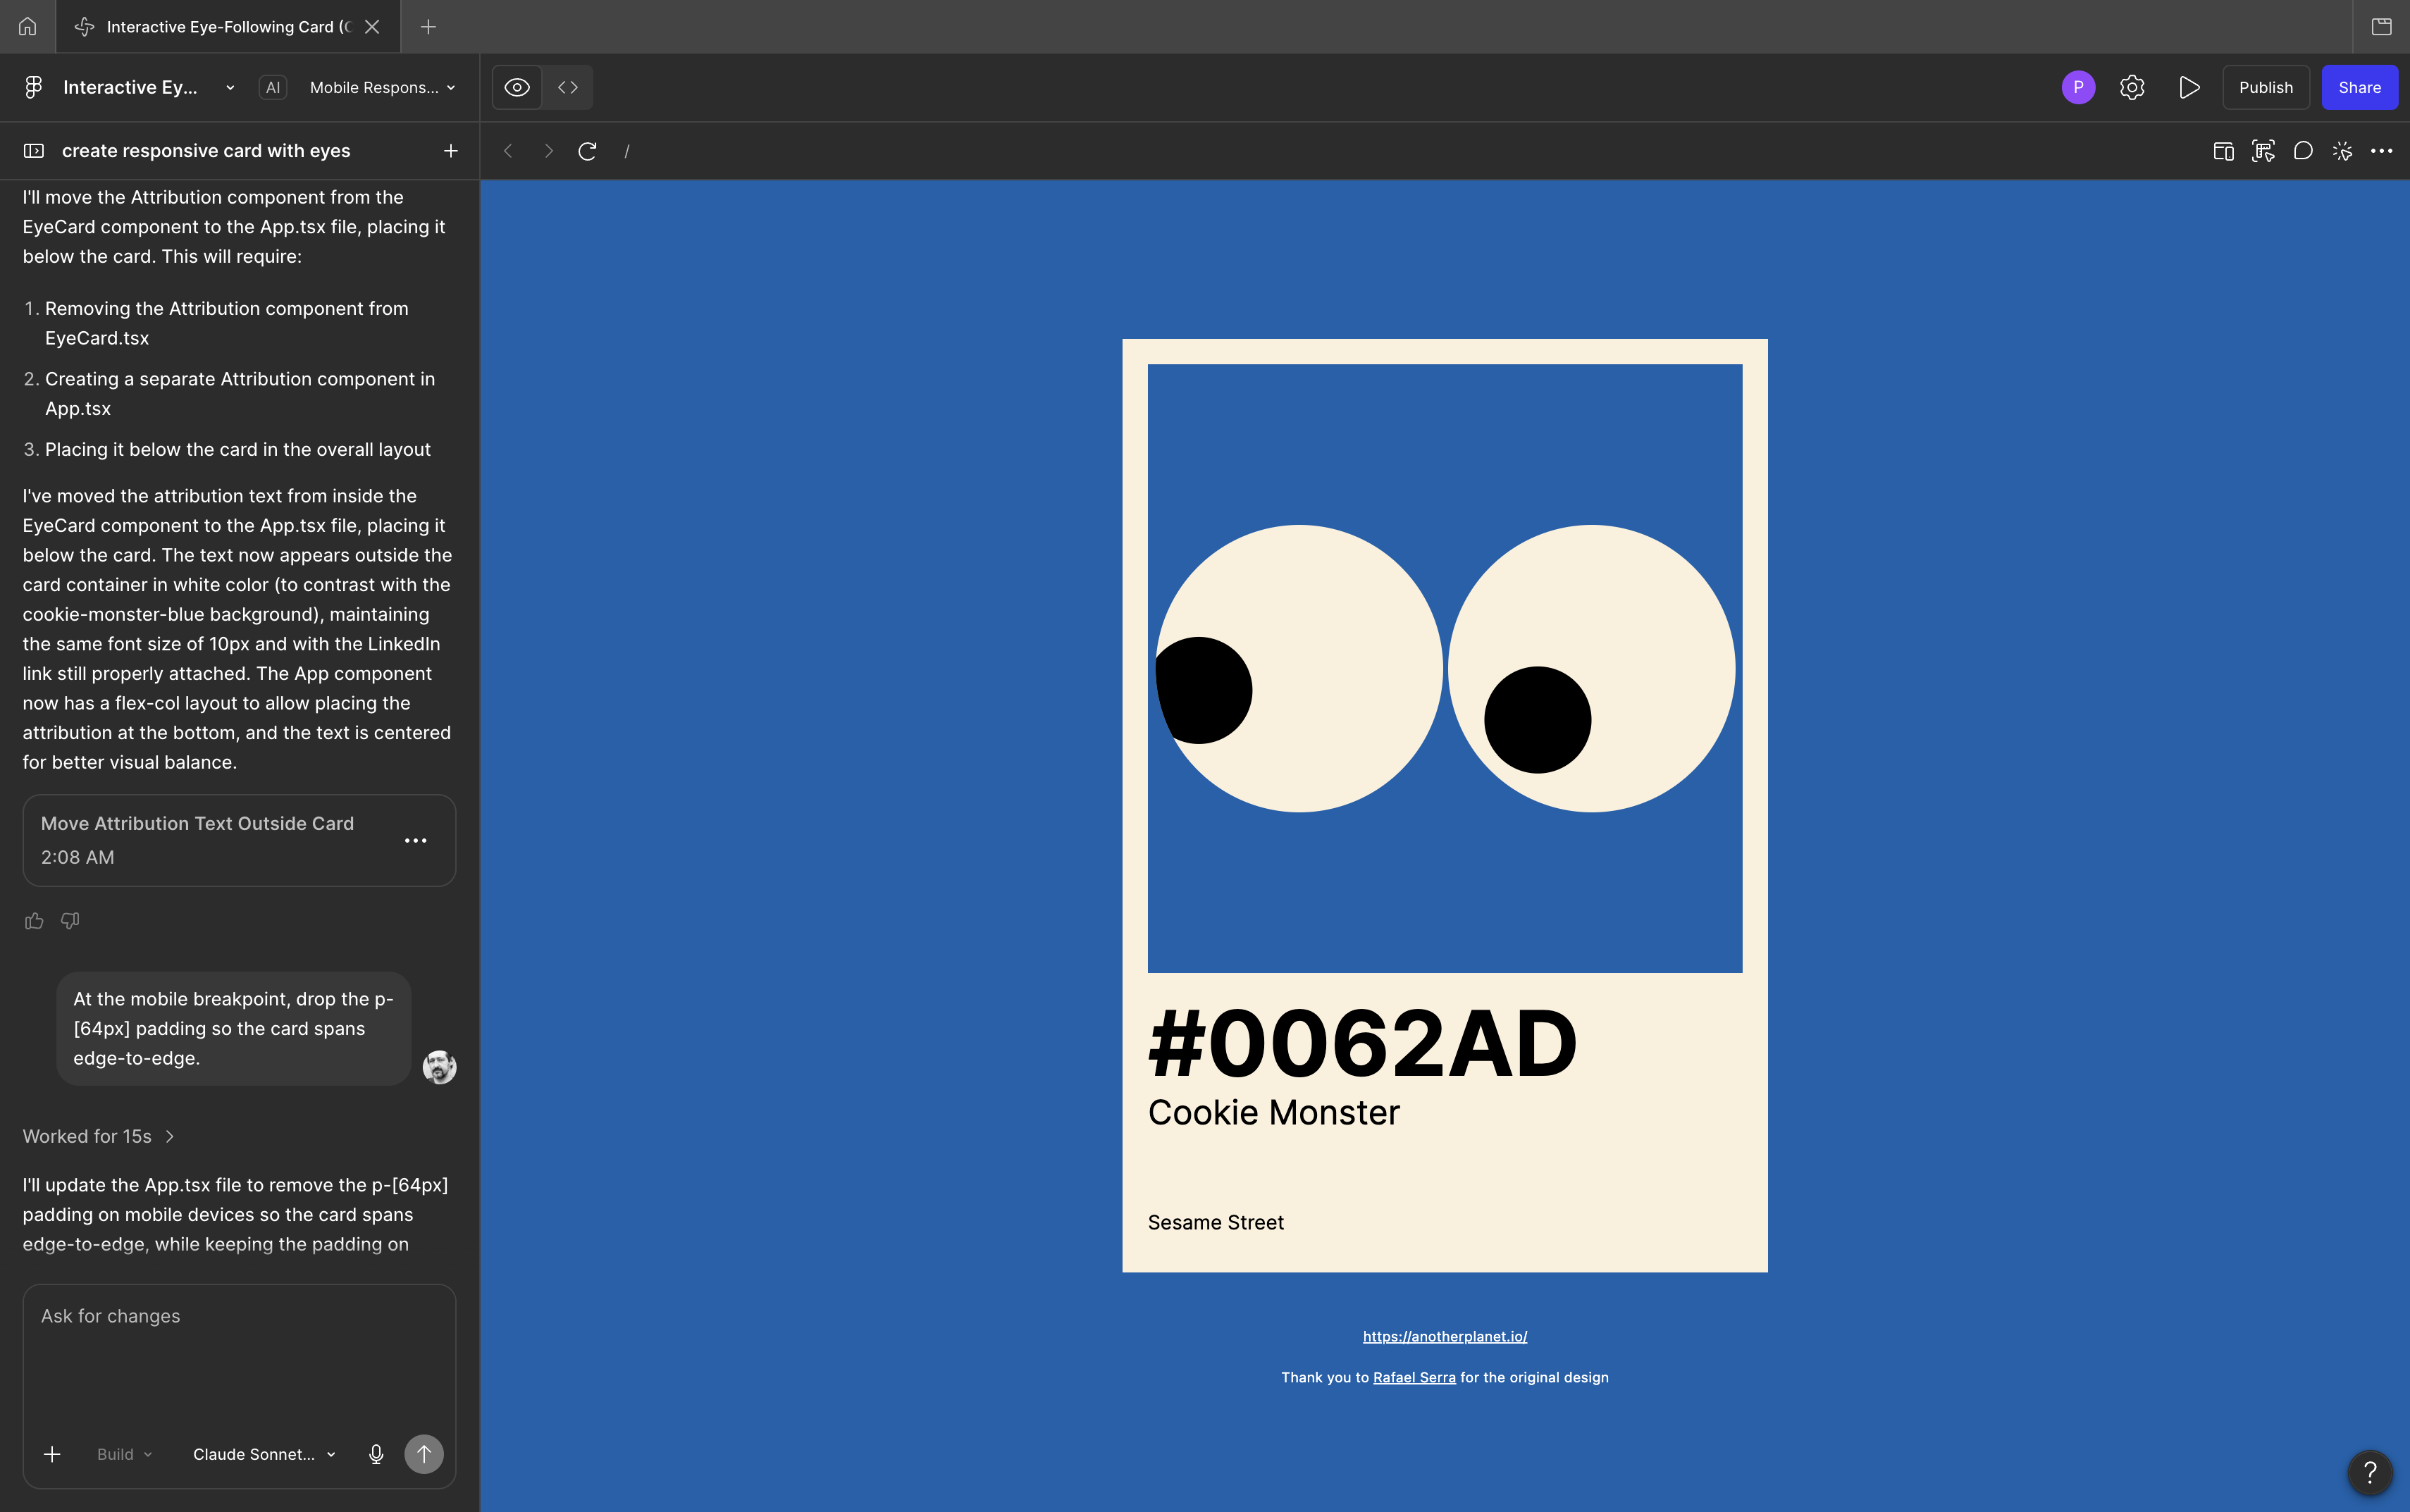
\includegraphics[
          width=0.5\textheight,
          height=0.95\linewidth,
          keepaspectratio,
          origin=c
        ]{figures/ch2-literature-review/figma-make.png}
        \caption{แพลตฟอร์ม Figma Make ใช้สำหรับสร้าง UI ด้วยภาษาธรรมชาติ}
        \label{fig:figma-make}
      \end{figure}

    \item \textbf{เครื่องมือตรวจงานด้วยหมุดคอมเมนต์ (เช่น BugHerd, Marker.io)} ให้ผู้ใช้ปักหมุดความคิดเห็นบนหน้าเว็บ พร้อมแนบภาพหน้าจอและข้อมูลทางเทคนิคโดยอัตโนมัติ~\cite{bugherd,markerio} และเริ่มนำ AI มาใช้จัดการข้อเสนอแนะแล้ว เช่น BugHerd เชื่อมต่อ AI agent ผ่าน MCP เพื่อช่วยคัดแยกงาน~\cite{bugherd_ai} แต่ยังขาดฟังก์ชันเปรียบเทียบสองทางเลือกและการจำแนกข้อเสนอแนะตามประเภทปัญหา
  \end{itemize}
}

\section{ภาษาคอมพิวเตอร์เเละเทคโนโลยี}

\subsection{แบบจำลองภาษาขนาดใหญ่ (Large Language Models: LLM)}

\thaijustify{
  แบบจำลองภาษาขนาดใหญ่ (Large Language Models: LLM) คือ เทคโนโลยีปัญญาประดิษฐ์ที่ฝึกด้วยข้อมูลข้อความจำนวนมาก ทำให้สามารถเข้าใจภาษาธรรมชาติ วิเคราะห์บริบท ให้เหตุผล และสร้างเนื้อหาหรือโค้ดได้ จึงสามารถนำมาช่วยลดภาระงานและสนับสนุนกระบวนการพัฒนาระบบได้อย่างมีประสิทธิภาพ
}

\thaijustify{
  โครงงานนี้ใช้ LLM ผ่าน CPE AI Gateway \cite{cpe_ai_gateway} สำหรับการสร้าง UI และประมวลผลภาษาธรรมชาติ โดยออกแบบกระบวนการแบบ AI Orchestration เพื่อเลือกโมเดลให้เหมาะสมกับแต่ละงาน โมเดลที่นำมาใช้ ได้แก่ muse-glimmer-30b และ qwen3.8-27b พร้อมเปรียบเทียบกับกลุ่ม Frontier Model เพื่อพิจารณาจุดเด่นและความเหมาะสมในการใช้งาน
}

% \thaijustify{
%   muse-glimmer-30b เป็นโมเดล open-weight ขนาดประมาณ 30 พันล้านพารามิเตอร์ที่มีความสมดุลระหว่างความสามารถในการให้เหตุผลและความเร็วในการประมวลผล โดยเฉพาะการสร้างผลลัพธ์แบบมีโครงสร้าง จึงเหมาะกับงาน Prompt-to-Design ที่แปลงคำสั่งภาษาธรรมชาติเป็นโครงสร้าง UI แบบสองทางเลือก (two-alternative UI) อีกทั้งยังใช้ทรัพยากรน้อยกว่าการใช้ Frontier Model ในทุกขั้นตอน \cite{meta2026museglimmer}
% }

\thaijustify{
   muse-glimmer-30b (Muse Glimmer) เป็นโมเดล open-weight ขนาดประมาณ 30 พันล้านพารามิเตอร์จาก Meta Superintelligence Labs ออกแบบมาสำหรับงานเอเจนต์ที่ทำงานต่อเนื่องบนเครื่องภายใน และรันบนฮาร์ดแวร์ระดับผู้บริโภคได้~\cite{meta2026museglimmer}จึงใช้ทรัพยากรน้อยกว่าการเรียกใช้ Frontier Model ในทุกขั้นตอน โครงงานนี้จึงเลือกใช้โมเดลนี้สำหรับงาน Prompt-to-Design ซึ่งแปลงคำสั่งภาษาธรรมชาติเป็นโครงสร้าง UI แบบสองทางเลือก (two-alternative UI)
}

% \thaijustify{
%   qwen3.8-27b เป็นโมเดลขนาด 27 พันล้านพารามิเตอร์ที่เด่นด้านการเข้าใจและประมวลผลภาษาธรรมชาติ จึงเหมาะกับการวิเคราะห์ข้อเสนอแนะจากผู้ทดสอบที่มักเป็นภาษาพูดและไม่มีโครงสร้าง ระบบสามารถใช้โมเดลนี้เพื่อสรุป จัดกลุ่ม และสกัดข้อมูลเชิงลึกจากข้อเสนอแนะเพื่อนำไปสร้าง Persona โดยใช้ทรัพยากรน้อยกว่าโมเดลขนาดใหญ่ \cite{qwentheam2026qwen38}
% }

\thaijustify{
  qwen3.8-27b (Qwen3.8-27B) เป็นโมเดล dense แบบ open-weight ขนาด 27 พันล้านพารามิเตอร์จาก Alibaba เผยแพร่ภายใต้สัญญาอนุญาต Apache~2.0 รับข้อมูลได้ทั้งข้อความ ภาพ และวิดีโอ มี context window 262,144 tokens ซึ่งขยายได้ถึงประมาณ 1 ล้าน tokens~\cite{qwentheam2026qwen38} context ที่ยาวนี้ทำให้ส่งข้อเสนอแนะจำนวนมากจากผู้เข้าร่วมทดสอบหลายคนเข้าไปวิเคราะห์ในคำขอเดียวได้ โครงงานนี้จึงใช้โมเดลนี้สรุป จัดกลุ่ม และสกัดข้อมูลเชิงลึกจากข้อเสนอแนะเพื่อนำไปสร้าง Persona Artifact ทั้งนี้ ผลการประเมินที่เผยแพร่ในช่วงเปิดตัวเป็นตัวเลขที่ผู้พัฒนาโมเดลรายงานเอง จึงต้องประเมินความสามารถของโมเดลกับข้อเสนอแนะภาษาไทย ซึ่งมักเป็นภาษาพูดและไม่มีโครงสร้าง
}

\thaijustify{
  และกลุ่ม Frontier Model มีตัวอย่างในช่วงที่จัดทำโครงงานนี้ ได้แก่ GPT-6 Astra ของ OpenAI ซึ่งเน้นความสามารถด้านการใช้งานคอมพิวเตอร์และวิศวกรรมซอฟต์แวร์ \cite{openai2026gpt6astra} Claude Opus 5.5 ของ Anthropic ซึ่งเน้นงานเขียนโค้ดแบบเอเจนต์ (Agentic Coding) และงานเชิงความรู้ \cite{anthropic2026opus55} และ Gemini 3.8 Flash ของ Google ซึ่งพัฒนาด้านวิศวกรรมซอฟต์แวร์และงานแบบเอเจนต์ โดยยังคงความเร็วสูงและต้นทุนต่ำ \cite{google2026gemini38flash} โมเดลกลุ่มนี้ให้คุณภาพผลลัพธ์สูงในงานที่ซับซ้อน แต่ส่วนใหญ่เป็นโมเดลแบบปิด (Closed-weight) ที่เข้าถึงได้ผ่าน API เชิงพาณิชย์เท่านั้น มีค่าใช้จ่ายตามจำนวนโทเคน และต้องส่งข้อมูลออกไปประมวลผลบนระบบภายนอก ซึ่งเป็นข้อพิจารณาสำคัญเมื่อข้อมูลที่ต้องประมวลผลคือข้อเสนอแนะของผู้เข้าร่วมทดสอบที่อยู่ภายใต้กฎหมายคุ้มครองข้อมูลส่วนบุคคล (PDPA) ด้วยเหตุนี้ โครงงานจึงใช้ Frontier Model เป็นเกณฑ์อ้างอิง (Baseline) ในการประเมินคุณภาพผลลัพธ์ของ muse-glimmer-30b และ qwen3.8-27b แทนการใช้เป็นโมเดลหลักในทุกขั้นตอน
}

\begin{table}[H]
  \centering
  \small
  \caption{เปรียบเทียบความสามารถและจุดด้อยของแบบจำลองภาษาขนาดใหญ่แต่ละรุ่น}
  \label{tab:ai-models-comparison}
  \begin{tabularx}{\textwidth}{
      >{\raggedright\arraybackslash}p{0.20\textwidth}
      |
      >{\raggedright\arraybackslash}X
      >{\raggedright\arraybackslash}X
      >{\raggedright\arraybackslash}X
    }
    \hhline{=|===}
    \textbf{Model} &
    \textbf{ประเภทงาน} &
    \textbf{จุดเด่น} &
    \textbf{จุดด้อย} \\
    \hhline{=|===}
    
    \texttt{muse-glimmer-30b} \newline \textit{(Context: 131K tokens)} &
    Prompt-to-Design และงานที่ต้องใช้การให้เหตุผล &
    มีความสามารถในการทำตามคำสั่งแบบมีโครงสร้าง (Structured output) ได้อย่างแม่นยำ ใช้ทรัพยากรน้อย และตอบสนองรวดเร็ว &
    ความสามารถในการวิเคราะห์ข้อมูลที่ซับซ้อนมาก ๆ หรือความรู้รอบกว้าง ยังเป็นรองโมเดลขนาดใหญ่ (Frontier Models) และมี Context Window ที่จำกัด \\

    \hline
    
    \texttt{qwen3.8-27b} \newline \textit{(Context: 256K - 1M tokens)} &
    การวิเคราะห์ข้อความ การสนทนา และการประมวลผลภาษาธรรมชาติ &
    เข้าใจภาษาพูดและบริบทที่คลุมเครือได้ดีเยี่ยม สรุปใจความ จัดกลุ่มข้อเสนอแนะ และดึงข้อมูลเชิงลึกได้อย่างเป็นธรรมชาติ &
    ขีดความสามารถด้านการคำนวณเชิงตรรกะซับซ้อน หรือการเขียนโค้ดขั้นสูง ยังไม่เทียบเท่ากลุ่ม Frontier Model \\

    \hline

    \texttt{Claude Opus 5.5} \newline \textit{(Frontier Model)} \newline \textit{(Context: 1M tokens)} &
    งานวิเคราะห์เชิงลึกขั้นสูง การเขียนและตรวจสอบโค้ดโปรแกรม &
    มีระบบ Adaptive thinking ที่ช่วยให้เหตุผลได้อย่างละเอียดลึกซึ้ง การใช้งานเครื่องมือ (Tools) มีความเสถียรและแม่นยำสูง &
    มีต้นทุนการเรียกใช้งาน (Cost) ที่ค่อนข้างสูง และระยะเวลาประมวลผล (Latency) อาจใช้เวลานานกว่าโมเดลทั่วไป \\

    \hline
    
    \texttt{Gemini 3.8 Flash} \newline \textit{(Frontier Model)} \newline \textit{(Context: 1M tokens)} &
    งานประมวลผลแบบ Multimodal และงานที่ต้องการผลลัพธ์แบบเรียลไทม์ &
    ประมวลผลได้อย่างรวดเร็วมาก (Fastest output) รองรับการรับข้อมูลทั้งข้อความ ภาพ เสียง และวิดีโอได้ดีเยี่ยมในราคาประหยัด &
    ประสิทธิภาพในการให้เหตุผลเชิงตรรกะสำหรับงานที่ซับซ้อนมาก ๆ อาจยังเป็นรองโมเดลในระดับ Pro หรือระดับที่สูงกว่า \\

    \hline
    
    \texttt{GPT-6 Astra} \newline \textit{(Frontier Model)} \newline \textit{(Context: 1M - 1.1M tokens)} &
    การประสานงานแบบ Multi-agent และการแก้ปัญหาที่ซับซ้อนขั้นสุด &
    มีศักยภาพการให้เหตุผลระดับสูงสุด สามารถควบคุมระบบคอมพิวเตอร์และทำงานซ้อนกันหลายขั้นตอน (Complex reasoning) ได้ดีเยี่ยม &
    มีต้นทุนการใช้งานที่สูงที่สุดในกลุ่ม อาจเกินความจำเป็นสำหรับระบบทั่วไป และมักมีข้อจำกัดด้านโควตาการใช้งานอย่างเข้มงวด \\

    \hline
  \end{tabularx}
\end{table}

% \begin{table}[H]
%   \centering
%   \small
%   \caption{เปรียบเทียบจุดเด่นและจุดด้อยของแบบจำลองภาษาขนาดใหญ่แต่ละรุ่น}
%   \label{tab:ai-models-comparison}
%   \begin{tabularx}{\textwidth}{
%       >{\raggedright\arraybackslash}p{0.20\textwidth}
%       |
%       >{\raggedright\arraybackslash}X
%       >{\raggedright\arraybackslash}X
%       >{\raggedright\arraybackslash}X
%     }
%     \hhline{=|===}
%     \textbf{Model} &
%     \textbf{ประเภทงาน} &
%     \textbf{จุดเด่น} &
%     \textbf{จุดด้อย} \\
%     \hhline{=|===}
 
%     % TODO: ยืนยัน context จาก https://huggingface.co/meta-models/Muse-Glimmer-30B
%     \texttt{muse-glimmer-30b} \newline \textit{(Context: 131K tokens)} &
%     Prompt-to-Design (สร้างและปรับปรุง two-alternative UI) &
%     โมเดล open-weight ขนาด 30B ที่ออกแบบมาสำหรับงานเอเจนต์ รันบนฮาร์ดแวร์ระดับผู้บริโภคได้ จึงใช้ทรัพยากรน้อย~\cite{meta2026museglimmer} &
%     Context window สั้นกว่ากลุ่ม Frontier Model และความแม่นยำในการสร้างผลลัพธ์แบบมีโครงสร้างสำหรับงาน Prompt-to-Design ยังต้องยืนยันด้วยชุดข้อมูลประเมินของโครงงาน \\
 
%     \hline
 
%     \texttt{qwen3.8-27b} \newline \textit{(Context: 262K ขยายได้ถึง 1M tokens)} &
%     การวิเคราะห์ สรุป และจัดกลุ่มข้อเสนอแนะ และการสังเคราะห์ข้อมูลสำหรับ Persona &
%     โมเดล dense แบบ open-weight (Apache~2.0) รับข้อมูลได้ทั้งข้อความ ภาพ และวิดีโอ มี context ยาวพอสำหรับรวมข้อเสนอแนะจำนวนมากในคำขอเดียว~\cite{qwentheam2026qwen38} &
%     ผลประเมินที่เผยแพร่ช่วงเปิดตัวเป็นตัวเลขที่ผู้พัฒนารายงานเอง และความสามารถกับข้อเสนอแนะภาษาไทยแบบภาษาพูดยังต้องประเมินด้วยชุดข้อมูลของโครงงาน \\
 
%     \hline
 
%     % TODO: ยืนยัน context ที่ https://platform.claude.com/docs/en/models/opus-5-5/overview
%     \texttt{Claude Opus 5.5} \newline \textit{(Frontier Model)} \newline \textit{(Context: 1M tokens)} &
%     งานวิเคราะห์เชิงลึก การเขียนโค้ดแบบเอเจนต์ และงานเชิงความรู้ &
%     ผู้พัฒนาระบุว่าเป็นรุ่น Opus ที่ทำงานด้านโค้ด เอเจนต์ และงานเชิงความรู้ได้ดีที่สุด ต้นทุนต่องานต่ำกว่า Opus~5 ราว 40\% และสร้างผลลัพธ์เร็วขึ้นกว่า 30\%~\cite{anthropic2026opus55} &
%     เป็นโมเดลแบบปิด (Closed-weight) ต้องส่งข้อมูลออกไปประมวลผลภายนอก และมีราคา 4/20 ดอลลาร์สหรัฐต่อล้าน tokens (input/output) ซึ่งสูงกว่าโมเดล open-weight มาก \\
 
%     \hline
 
%     % TODO: ยืนยัน context ของรุ่น Flash (หน้า docs ที่พบระบุ 1,048,576 tokens สำหรับรุ่น Flash Cyber)
%     \texttt{Gemini 3.8 Flash} \newline \textit{(Frontier Model)} \newline \textit{(Context: 1M tokens)} &
%     งานวิศวกรรมซอฟต์แวร์ งานแบบเอเจนต์ และงานที่ต้องการผลลัพธ์รวดเร็ว &
%     พัฒนาด้านวิศวกรรมซอฟต์แวร์และงานแบบเอเจนต์ โดยคงความเร็วสูงและต้นทุนต่ำ~\cite{google2026gemini38flash} &
%     % TODO: ช่องนี้ยังไม่มีแหล่งรองรับ
%     ประสิทธิภาพในการให้เหตุผลสำหรับงานที่ซับซ้อนมาก ๆ อาจยังเป็นรองโมเดลระดับ Pro หรือสูงกว่า \\
 
%     \hline
 
%     % TODO: ยืนยัน context จากหน้า model ของ OpenAI API
%     \texttt{GPT-6 Astra} \newline \textit{(Frontier Model)} \newline \textit{(Context: 1M - 1.1M tokens)} &
%     งานที่ใช้คอมพิวเตอร์ (Computer use) วิศวกรรมซอฟต์แวร์ และงานวิชาชีพที่ซับซ้อน &
%     ผู้พัฒนาระบุว่าทำผลงานระดับ state-of-the-art ด้าน computer use, browsing, วิศวกรรมซอฟต์แวร์ และงานวิชาชีพ~\cite{openai2026gpt6astra} &
%     % TODO: ยืนยันราคาจากหน้า pricing ทางการของ OpenAI
%     มีต้นทุนการใช้งานสูงที่สุดในกลุ่ม (10/50 ดอลลาร์สหรัฐต่อล้าน tokens) และอาจเกินความจำเป็นสำหรับระบบทั่วไป \\
 
%     \hline
%   \end{tabularx}
% \end{table}

\thaijustify{
  ในกระบวนการทำงาน AI Orchestration จะเลือกโมเดลตามประเภทของงาน เช่น คำขอที่เกี่ยวข้องกับการสร้างหรือปรับปรุง UI จากความต้องการทางการออกแบบจะถูกส่งไปยัง muse-glimmer-30b ขณะที่งานสนทนา การสรุปและการวิเคราะห์ข้อเสนอแนะ รวมถึงการสังเคราะห์ข้อมูลสำหรับ Persona Artifact จะใช้ qwen3.8-27b เป็นหลัก
}
\thaijustify{
  การแบ่งหน้าที่ดังกล่าวช่วยให้แต่ละโมเดลถูกใช้งานตามความสามารถที่เหมาะสมและทำให้กระบวนการประมวลผลของระบบมีโครงสร้างชัดเจนมากกว่าการใช้โมเดลเดียวสำหรับงานทุกประเภท
}

\subsection{เทคโนโลยีการสร้างส่วนต่อประสานผู้ใช้โดยกำหนด Design System}
\thaijustify{
  งานวิจัยที่ศึกษาการให้ Generative AI สร้าง UI ให้ตรงกับ design system มีการศึกษาเชิงเปรียบเทียบ context engineering สามแบบสำหรับ LLM agent ได้แก่ instruction-based, context-based และ registry-based \cite{designsystem_compliant_ui_2026} ผลพบว่าการให้ agent ใช้ component สำเร็จรูปจาก registry ให้ความสอดคล้องกับ design system สูงและขยายขนาดได้ดีกว่า เพราะเปลี่ยนจากการให้ LLM ตีความข้อความไปเป็นการตรวจสอบระดับ component และมีงานอีกกลุ่มหนึ่งใช้ข้อจำกัดด้านการออกแบบเป็นตัวกำหนด เช่น UIDEC~\cite{uidec_2025} ที่ให้นักออกแบบระบุรายละเอียดโครงการ ได้แก่ วัตถุประสงค์ กลุ่มเป้าหมาย อุตสาหกรรม และสไตล์การออกแบบ แล้วใช้ Generative AI สร้างตัวอย่างการออกแบบที่หลากหลายภายใต้ข้อจำกัดนั้นโดยนักออกแบบแทบไม่ต้องเขียน prompt เอง และ PrototypeFlow~\cite{prototypeflow_humanai_ui_design} ที่สร้าง theme ที่แก้ไขได้และดึงความรู้ด้านการออกแบบมาช่วยให้สี สไตล์ และ layout มีความสอดคล้องกัน จากบทความเหล่านี้ โครงงานนี้จึงนำแนวคิดนี้มาประยุกต์ใช้ในการสร้าง component และ material ที่ทำหน้าที่เป็นโครงสร้างพื้นฐานให้ LLM หรือนักพัฒนาสามารถนำไปหยิบใช้และทำงานต่อได้ทันทีโดยไม่ต้องเสียเวลาเขียนโค้ดหรือจัดการรายละเอียดด้วยตนเองอีกครั้ง
}

\section{สรุปการศึกษาค้นคว้า}

% \begin{table}[H]
%   \centering
%   \small
%   \caption{สรุปประเด็นจากงานวิจัยและเครื่องมือที่เกี่ยวข้อง}
%   \label{tab:literature_summary}
%   \begin{tabularx}{\textwidth}{
%       >{\raggedright\arraybackslash}p{0.18\textwidth}
%       >{\raggedright\arraybackslash}p{0.22\textwidth}
%       >{\raggedright\arraybackslash}X
%       >{\raggedright\arraybackslash}X
%     }
%     \hline
%     \textbf{กลุ่มประเด็น} &
%     \textbf{งานที่เกี่ยวข้อง} &
%     \textbf{สิ่งที่มีการศึกษาแล้ว} &
%     \textbf{ช่องว่างที่พบ} \\
%     \hline

%     การสร้าง UI และต้นแบบด้วย Generative AI &
%     \cite{suh2025storyensemble, feng2023designing, yuan2024towards, kolthoff2024} &
%     Generative AI สามารถช่วยสร้าง wireframe, prototype และทางเลือกของ UI
%     จากความต้องการของนักออกแบบ เพื่อลดเวลาและแรงงานในการสร้างต้นแบบ
%     และช่วยให้สามารถสำรวจทางเลือกของการออกแบบได้มากขึ้น &
%     ผลลัพธ์ที่สร้างโดย Generative AI ยังพบปัญหาด้าน layout, style และการตีความ
%     function ที่ไม่ตรงกับความต้องการ รวมถึงยังไม่ได้เชื่อมกับกระบวนการ
%     ทดสอบและปรับปรุงจากข้อเสนอแนะของผู้ใช้อย่างครบวงจร \\

%     \hline

%     การทดสอบและการสกัดความต้องการจากต้นแบบ &
%     \cite{nielsen2000five, virzi1992refining,
%     nielsen1993mathematical, pacheco2018, lu2026} &
%     การทดสอบกับผู้ใช้กลุ่มเล็กหลายรอบสามารถช่วยค้นพบปัญหาได้อย่างมีประสิทธิภาพ
%     และการใช้ prototype ช่วยให้นักออกแบบสามารถสกัดความต้องการและรับ
%     ข้อเสนอแนะก่อนพัฒนาระบบจริงได้ &
%     การทำการทดสอบซ้ำหลายรอบยังสร้างภาระในการเตรียมหลายรูปแบบของ UI
%     รวบรวมข้อเสนอแนะ และนำผลจากแต่ละรอบกลับไปปรับปรุงการออกแบบ \\

%     \hline

%     การตีความข้อเสนอแนะและการสร้าง User Persona &
%     \cite{nngroup_satisfaction, nngroup_qualitative,
%     shukla2025, mitchell1997, shin2024} &
%     งานวิจัยแสดงให้เห็นว่าความชอบของผู้ใช้อาจไม่ตรงกับปัญหาการใช้งานจริง
%     และข้อเสนอแนะยังแตกต่างกันตามบทบาทและความต้องการของผู้ให้ข้อมูล
%     นอกจากนี้ LLM สามารถช่วยสรุปข้อมูลเพื่อสร้าง User Persona ได้
%     แต่ยังต้องอาศัยมนุษย์ในการระบุและตรวจสอบลักษณะที่สำคัญของผู้ใช้ &
%     ยังต้องมีกระบวนการเชื่อมโยงข้อเสนอแนะกับกลุ่มผู้ใช้
%     แยกความต้องการและความชอบออกจากกัน และนำข้อมูลเหล่านี้ไปสังเคราะห์
%     เป็น Persona ที่นักออกแบบสามารถตรวจสอบและนำกลับไปใช้ในการออกแบบได้ \\

%     \hline

%     การใช้ปัญญาประดิษฐ์วิเคราะห์ข้อเสนอแนะร่วมกับมนุษย์ &
%     \cite{gao2024collabcoder, gebreegziabher2023patat,
%     song2025, amershi2019, pourasad2025} &
%     LLM สามารถช่วยจัดกลุ่ม สรุป และวิเคราะห์ข้อมูลเชิงคุณภาพได้
%     แต่ยังมีข้อจำกัดด้านอคติและอาจพลาดข้อมูลสำคัญ
%     งานวิจัยจึงสนับสนุนการให้มนุษย์เข้ามาตรวจสอบและตัดสินใจร่วมกับปัญญาประดิษฐ์ &
%     จำเป็นต้องมีกระบวนการที่ให้นักออกแบบตรวจสอบ แก้ไข
%     และยืนยันผลการวิเคราะห์ของปัญญาประดิษฐ์ก่อนที่ผลลัพธ์จะถูกนำไปใช้
%     ปรับปรุงงานออกแบบ \\

%     \hline

%     เครื่องมือที่มีอยู่ในปัจจุบัน &
%     \cite{kameleoon, otterab, lyssna, useberry,
%     figma_agent, bugherd, markerio} &
%     เครื่องมือแต่ละประเภทสนับสนุนบางส่วนของกระบวนการ เช่น
%     การทดสอบหลายรูปแบบ การทดสอบ prototype การสร้าง UI ด้วย AI
%     หรือการให้ข้อเสนอแนะบนงานออกแบบ &
%     ความสามารถเหล่านี้ยังแยกอยู่ในหลายเครื่องมือ
%     และยังไม่มีการเชื่อมตั้งแต่การสร้างทางเลือกของ UI
%     การทดสอบ การวิเคราะห์ข้อเสนอแนะ การสร้าง Persona
%     จนถึงการนำผลกลับไปใช้ในรอบการออกแบบถัดไป \\

%     \hline
%   \end{tabularx}
% \end{table}

\thaijustify{
  จากการศึกษางานวิจัยและเครื่องมือที่เกี่ยวข้อง พบว่าแต่ละแนวทางสามารถสนับสนุนบางส่วนของ UX/UI DLC ได้แล้ว แต่กระบวนการตั้งแต่
  การสร้างต้นแบบ การทดสอบกับผู้ใช้ การรวบรวมและวิเคราะห์ข้อเสนอแนะจนถึงการนำข้อมูลกลับไปปรับปรุงการออกแบบยังคงแยกออกจากกัน
}
\thaijustify{
  ดังนั้น โครงงานนี้จึงมุ่งเชื่อมกระบวนการเหล่านี้เข้าด้วยกันโดยใช้ Generative AI ช่วยสร้าง two-alternative UI จากความต้องการทางการออกแบบ แล้วนำไปทำ Comparative Usability Test และให้ผู้เข้าร่วมทดสอบสามารถให้ข้อเสนอแนะลงบน component ได้โดยตรง จากนั้นระบบจะช่วยรวบรวมและวิเคราะห์ข้อเสนอแนะเพื่อค้นหาปัญหา ความต้องการ ความชอบและลักษณะร่วมของผู้ใช้แต่ละกลุ่ม เพื่อนำไปสนับสนุนการสร้าง Persona Artifact โดยให้นักออกแบบเป็นผู้ตรวจสอบและตัดสินใจผลลัพธ์ก่อนนำข้อมูลที่ผ่านการยืนยันแล้วกลับไปใช้ในการสร้างและทดสอบรอบถัดไป
}
\thaijustify{
  แนวทางดังกล่าวทำให้ โครงงานไม่ได้มุ่งใช้ Generative AI เพื่อสร้าง two-alternative UI เพียงอย่างเดียว แต่ใช้ปัญญาประดิษฐ์เพื่อสนับสนุน UX/UI DLC ตั้งแต่การสร้างต้นแบบ การทดสอบการใช้งาน ไปจนถึงการนำความต้องการ
  ของผู้ใช้กลับมาใช้ในการตัดสินใจเชิงออกแบบ โดยยังคงให้นักออกแบบเป็นผู้ควบคุมการตัดสินใจในแต่ละรอบ
}

% \thaijustify{
%   และจากการทบทวนวรรณกรรมทำให้เห็นช่องว่างทางการวิจัย คือ ปัจจุบันยังไม่มีเครื่องมือหรืองานวิจัยใดที่รวบรวมความสามารถทั้ง 4 ด้านไว้ในระบบเดียว ได้แก่ (1) การใช้ปัญญาประดิษฐ์สร้าง two-alternative UI ภายใต้ Design system ที่กำหนด (2) การให้ผู้ทดสอบให้ข้อเสนอแนะ (3) การใช้ปัญญาประดิษฐ์แยกแยะ pain point ออกจากความชอบร่วมกับการตัดสินใจของนักออกแบบ และ (4) การสร้าง Persona Artifact จากผลลัพธ์
% }
% \thaijustify{สิ่งที่โครงงานนี้ควรให้ความสำคัญเป็น คือ การพัฒนาแพลตฟอร์มนี้ให้ครอบคลุมกระบวนการตั้งแต่รับโจทย์ สร้างต้นแบบ รวบรวมข้อเสนอแนะ และวิเคราะห์ผลลัพธ์ เพื่อให้นักออกแบบสามารถส่งมอบงานที่มีการตรวจสอบความต้องการของผู้ใช้ที่แท้จริง พร้อมด้วย design system และต้นแบบที่ลูกค้าพึงพอใจให้นักพัฒนาต่อไปได้อย่างมีประสิทธิภาพ
% }


% !TeX root = ../../../proposal.tex
% Chapter 3: Methodology
\chapter{วิธีการดำเนินงาน}
\thaijustify{
  ในบทที่ 3 จะกล่าวถึงภาพรวมการออกแบบสถาปัตยกรรมระบบและแผนภาพแสดงกรณีการใช้งาน (Use case diagram) ของโครงงาน
}
\begin{samepage}
  \section{Preliminary Use Case Diagram}
  \thaijustify{
    แผนภาพกรณีการใช้งาน (Use case diagram) แสดงความสัมพันธ์ระหว่างผู้ใช้งานแต่ละบทบาทกับฟังก์ชันของแพลตฟอร์ม โดยแบ่งออกเป็น 4 ส่วน ได้แก่ ส่วน Authentication, ส่วนสร้าง two-alternative UI, ส่วนทดสอบการใช้งานและรับความเห็น, และส่วนสร้างรายงาน
  }
  \subsection{Authentication}
  \begin{figure}[H]
    \centering
    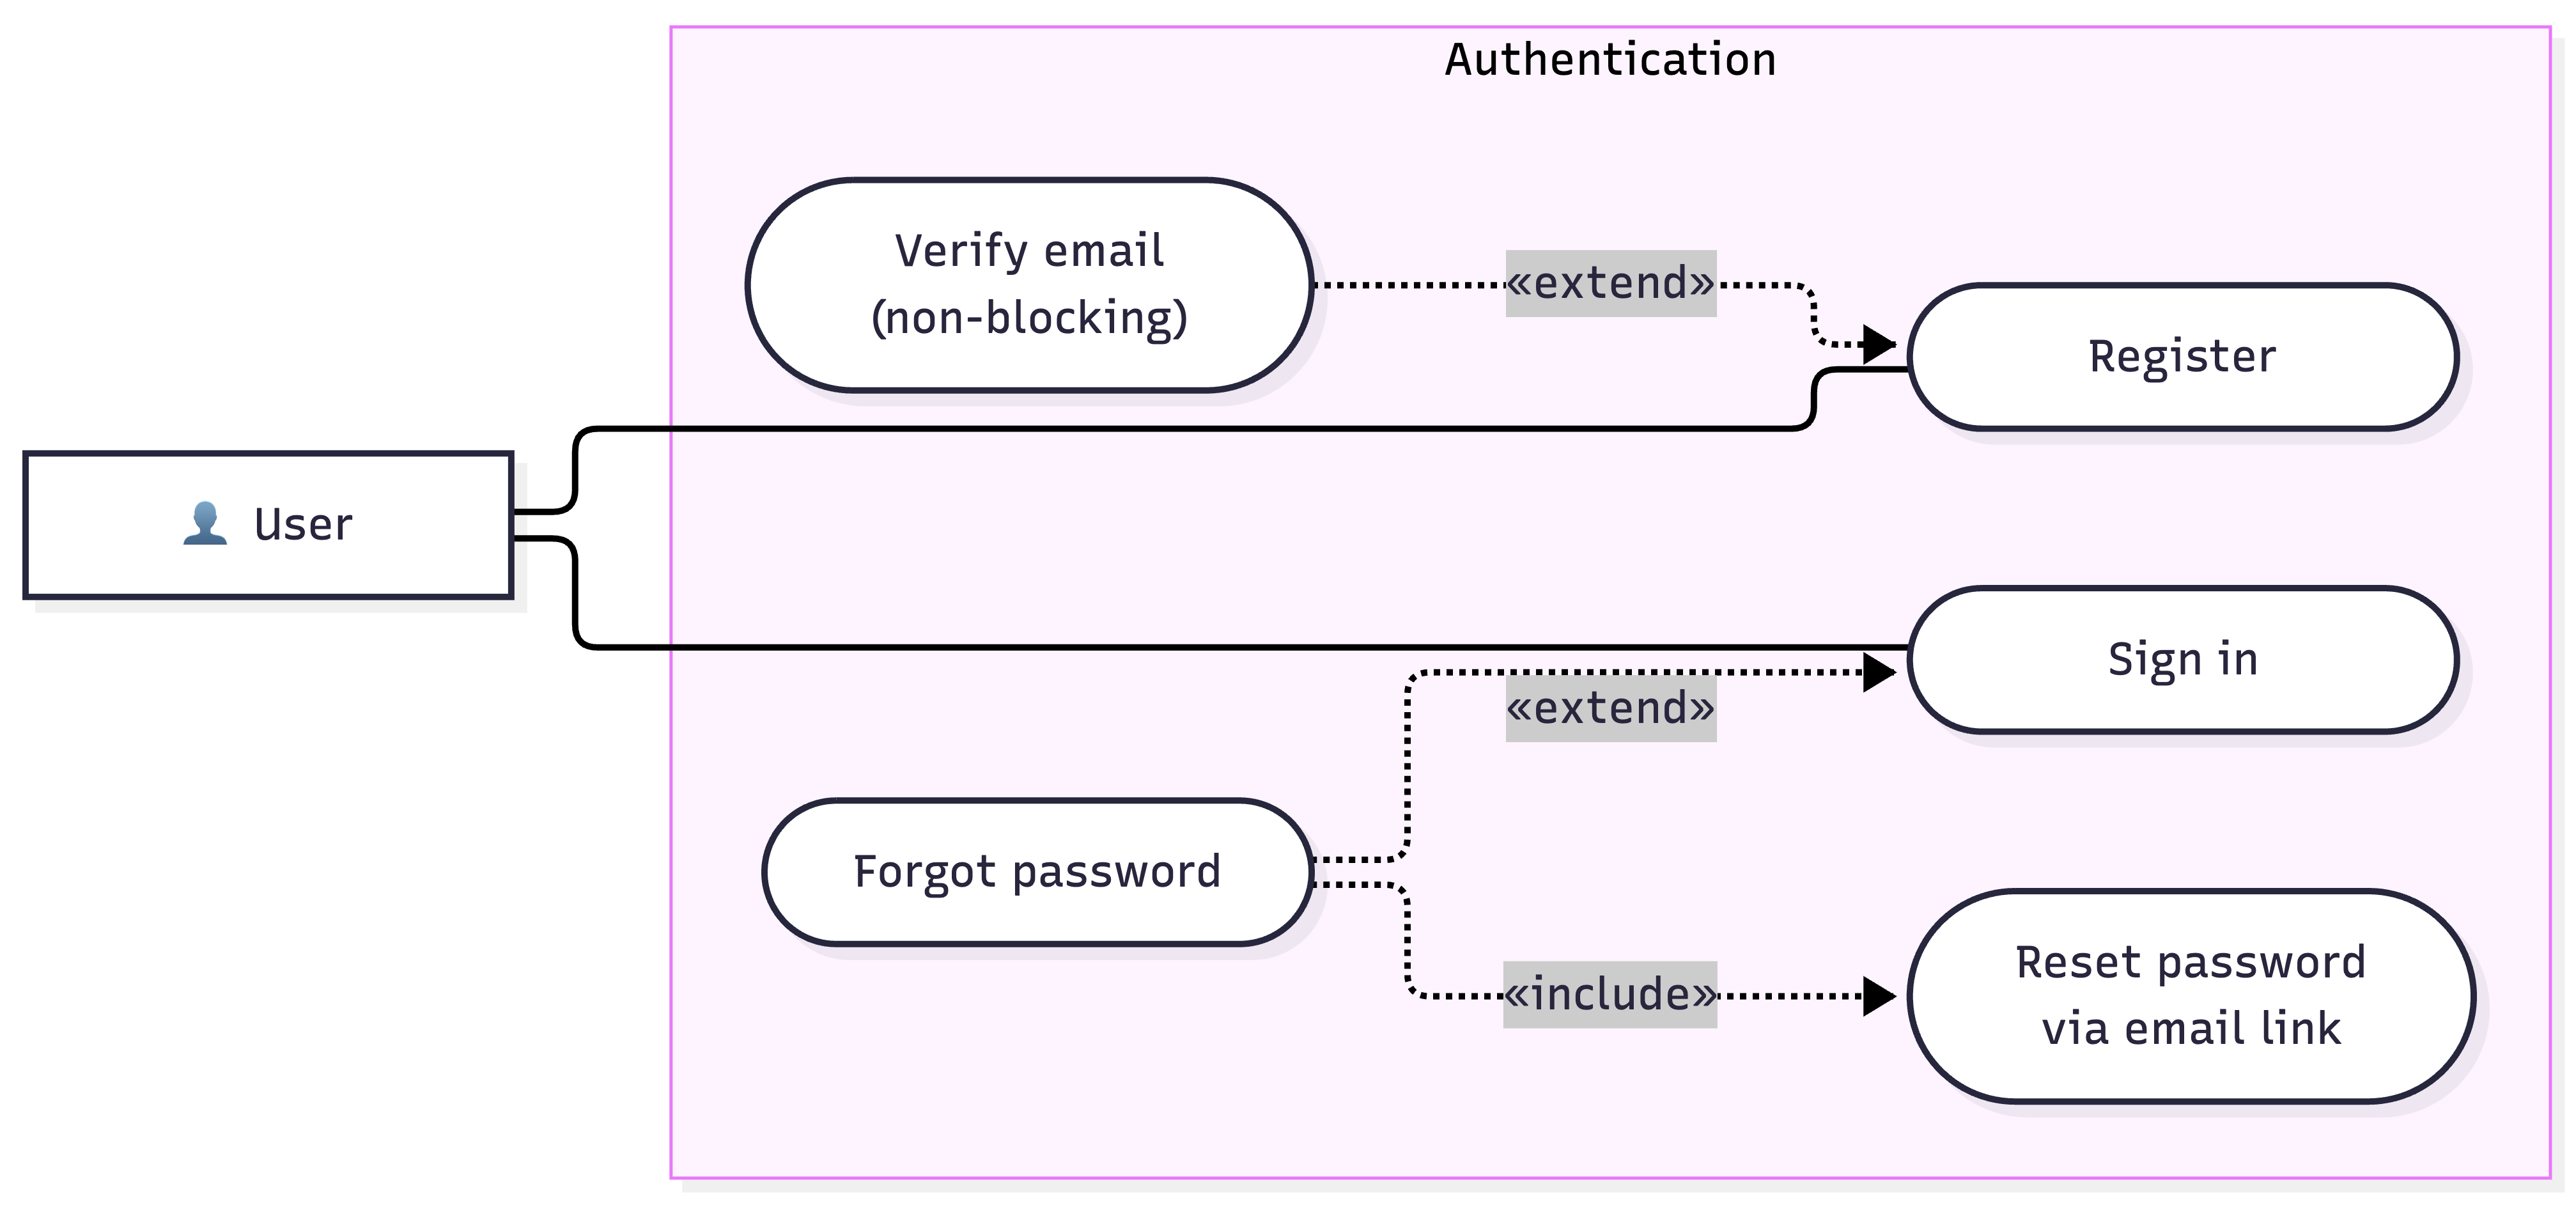
\includegraphics[
      width=0.6\textheight,
      height=\linewidth,
      keepaspectratio,
      origin=c
    ]{figures/ch3-methodology/UC-1.png}
    \caption{Use case diagram for authentication}
    \label{fig:UC-1}
    \thaijustify{ภาพแสดง Use Case ของระบบ Authentication โดยผู้ใช้สามารถสมัครสมาชิก เข้าสู่ระบบ และกู้คืนรหัสผ่านได้ โดยการยืนยันอีเมลเป็นขั้นตอนเสริมหลังการสมัคร และการรีเซ็ตรหัสผ่านดำเนินการผ่านลิงก์ที่ส่งทางอีเมล}
  \end{figure}
  \subsection{Designer: Project setup \& UI Generation}
  \begin{figure}[H]
    \centering
    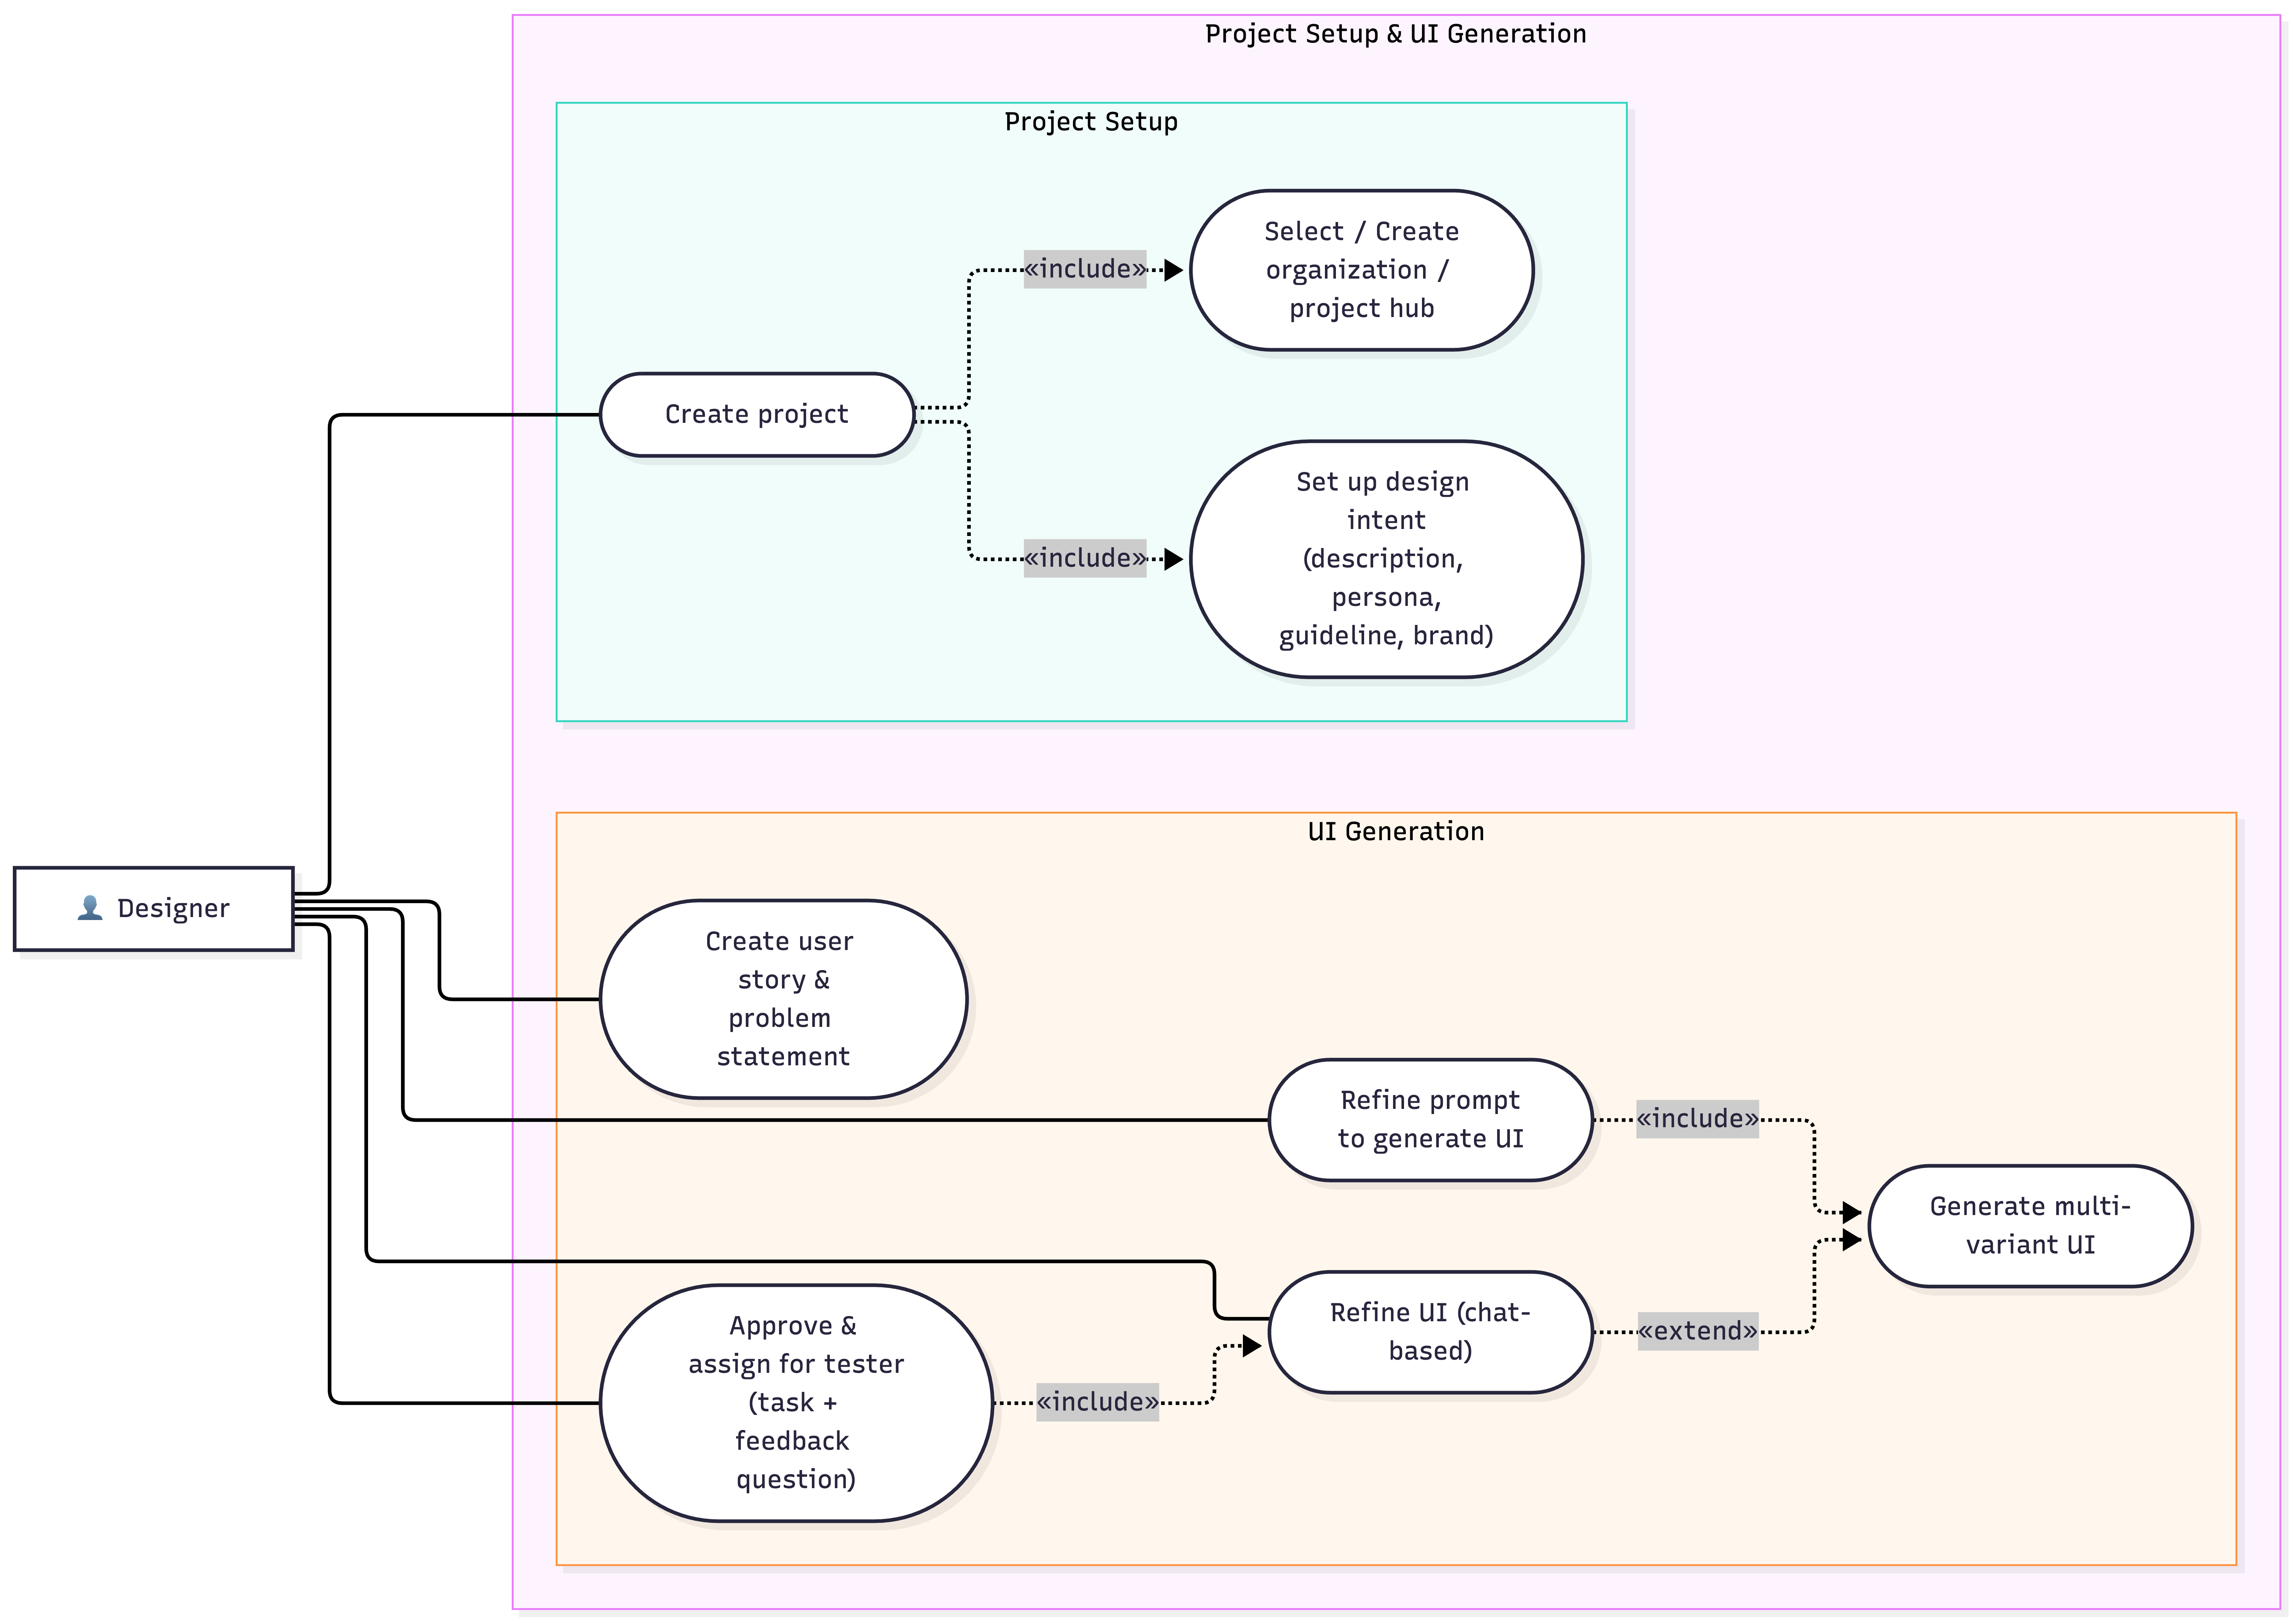
\includegraphics[
      width=0.6\textheight,
      height=\linewidth,
      keepaspectratio,
      origin=c
    ]{figures/ch3-methodology/UC-2.png}
    \caption{Use case diagram for Project setup and UI Generation}
    \label{fig:UC-2}
    \thaijustify{ภาพแสดง Use Case ของกระบวนการจัดเตรียมโครงการและสร้าง UI โดย Designer สามารถสร้างโครงการ กำหนด Design Intent สร้างและปรับแต่ง Prompt เพื่อสร้าง UI หลายรูปแบบ รวมถึงปรับแก้ UI และอนุมัติเพื่อส่งให้ผู้ทดสอบประเมิน}
  \end{figure}
  \subsection{Designer and Tester: Testing session and Feedback analysis}
  \begin{figure}[H]
    \centering
    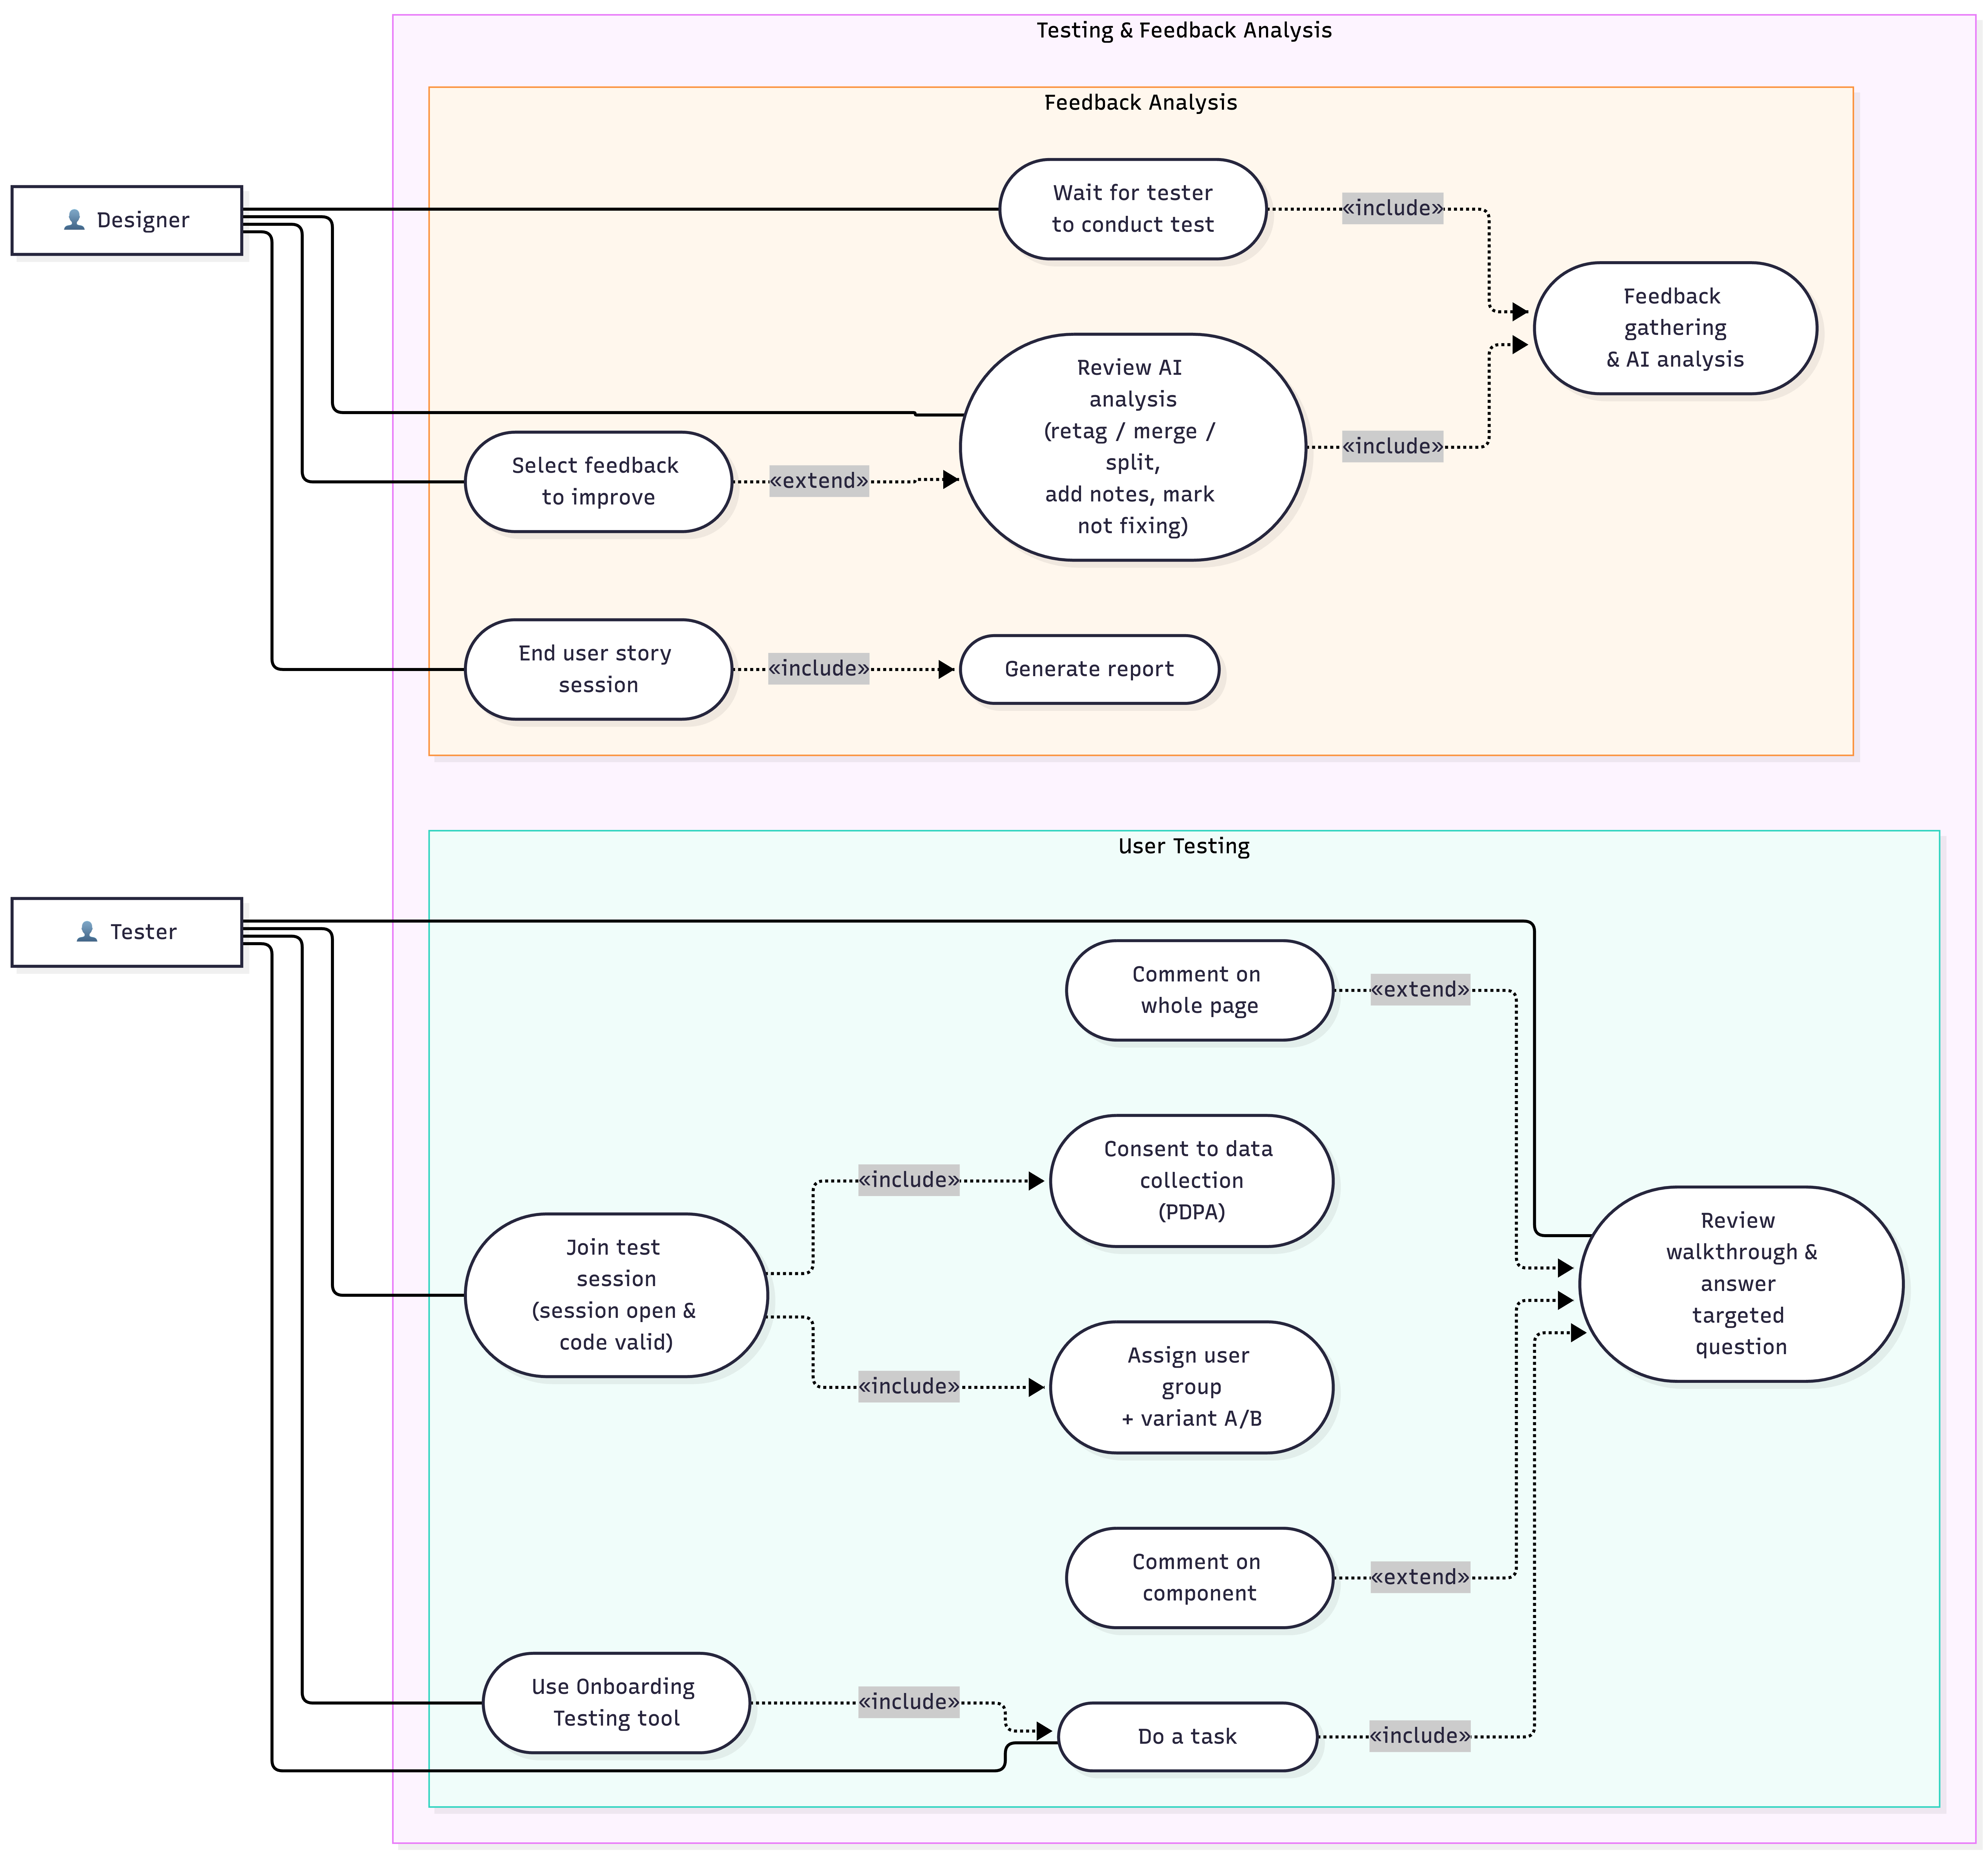
\includegraphics[
      width=0.6\textheight,
      height=\linewidth,
      keepaspectratio,
      origin=c
    ]{figures/ch3-methodology/UC-3.png}
    \caption{Use case diagram for Testing session and Feedback analysis}
    \label{fig:UC-3}
    \thaijustify{ภาพแสดง Use Case ของกระบวนการทดสอบและวิเคราะห์ Feedback โดย Tester เข้าร่วมการทดสอบ ทำภารกิจ และให้ความคิดเห็น ขณะที่ Designer รวบรวมและตรวจสอบผลการทดสอบ วิเคราะห์ Feedback ด้วย AI และเลือกประเด็นเพื่อนำไปปรับปรุงส่วนต่อประสานผู้ใช้}
  \end{figure}
  \subsection{Client, Developer, and Project Manager: Project view and Report}
  \begin{figure}[H]
    \centering
    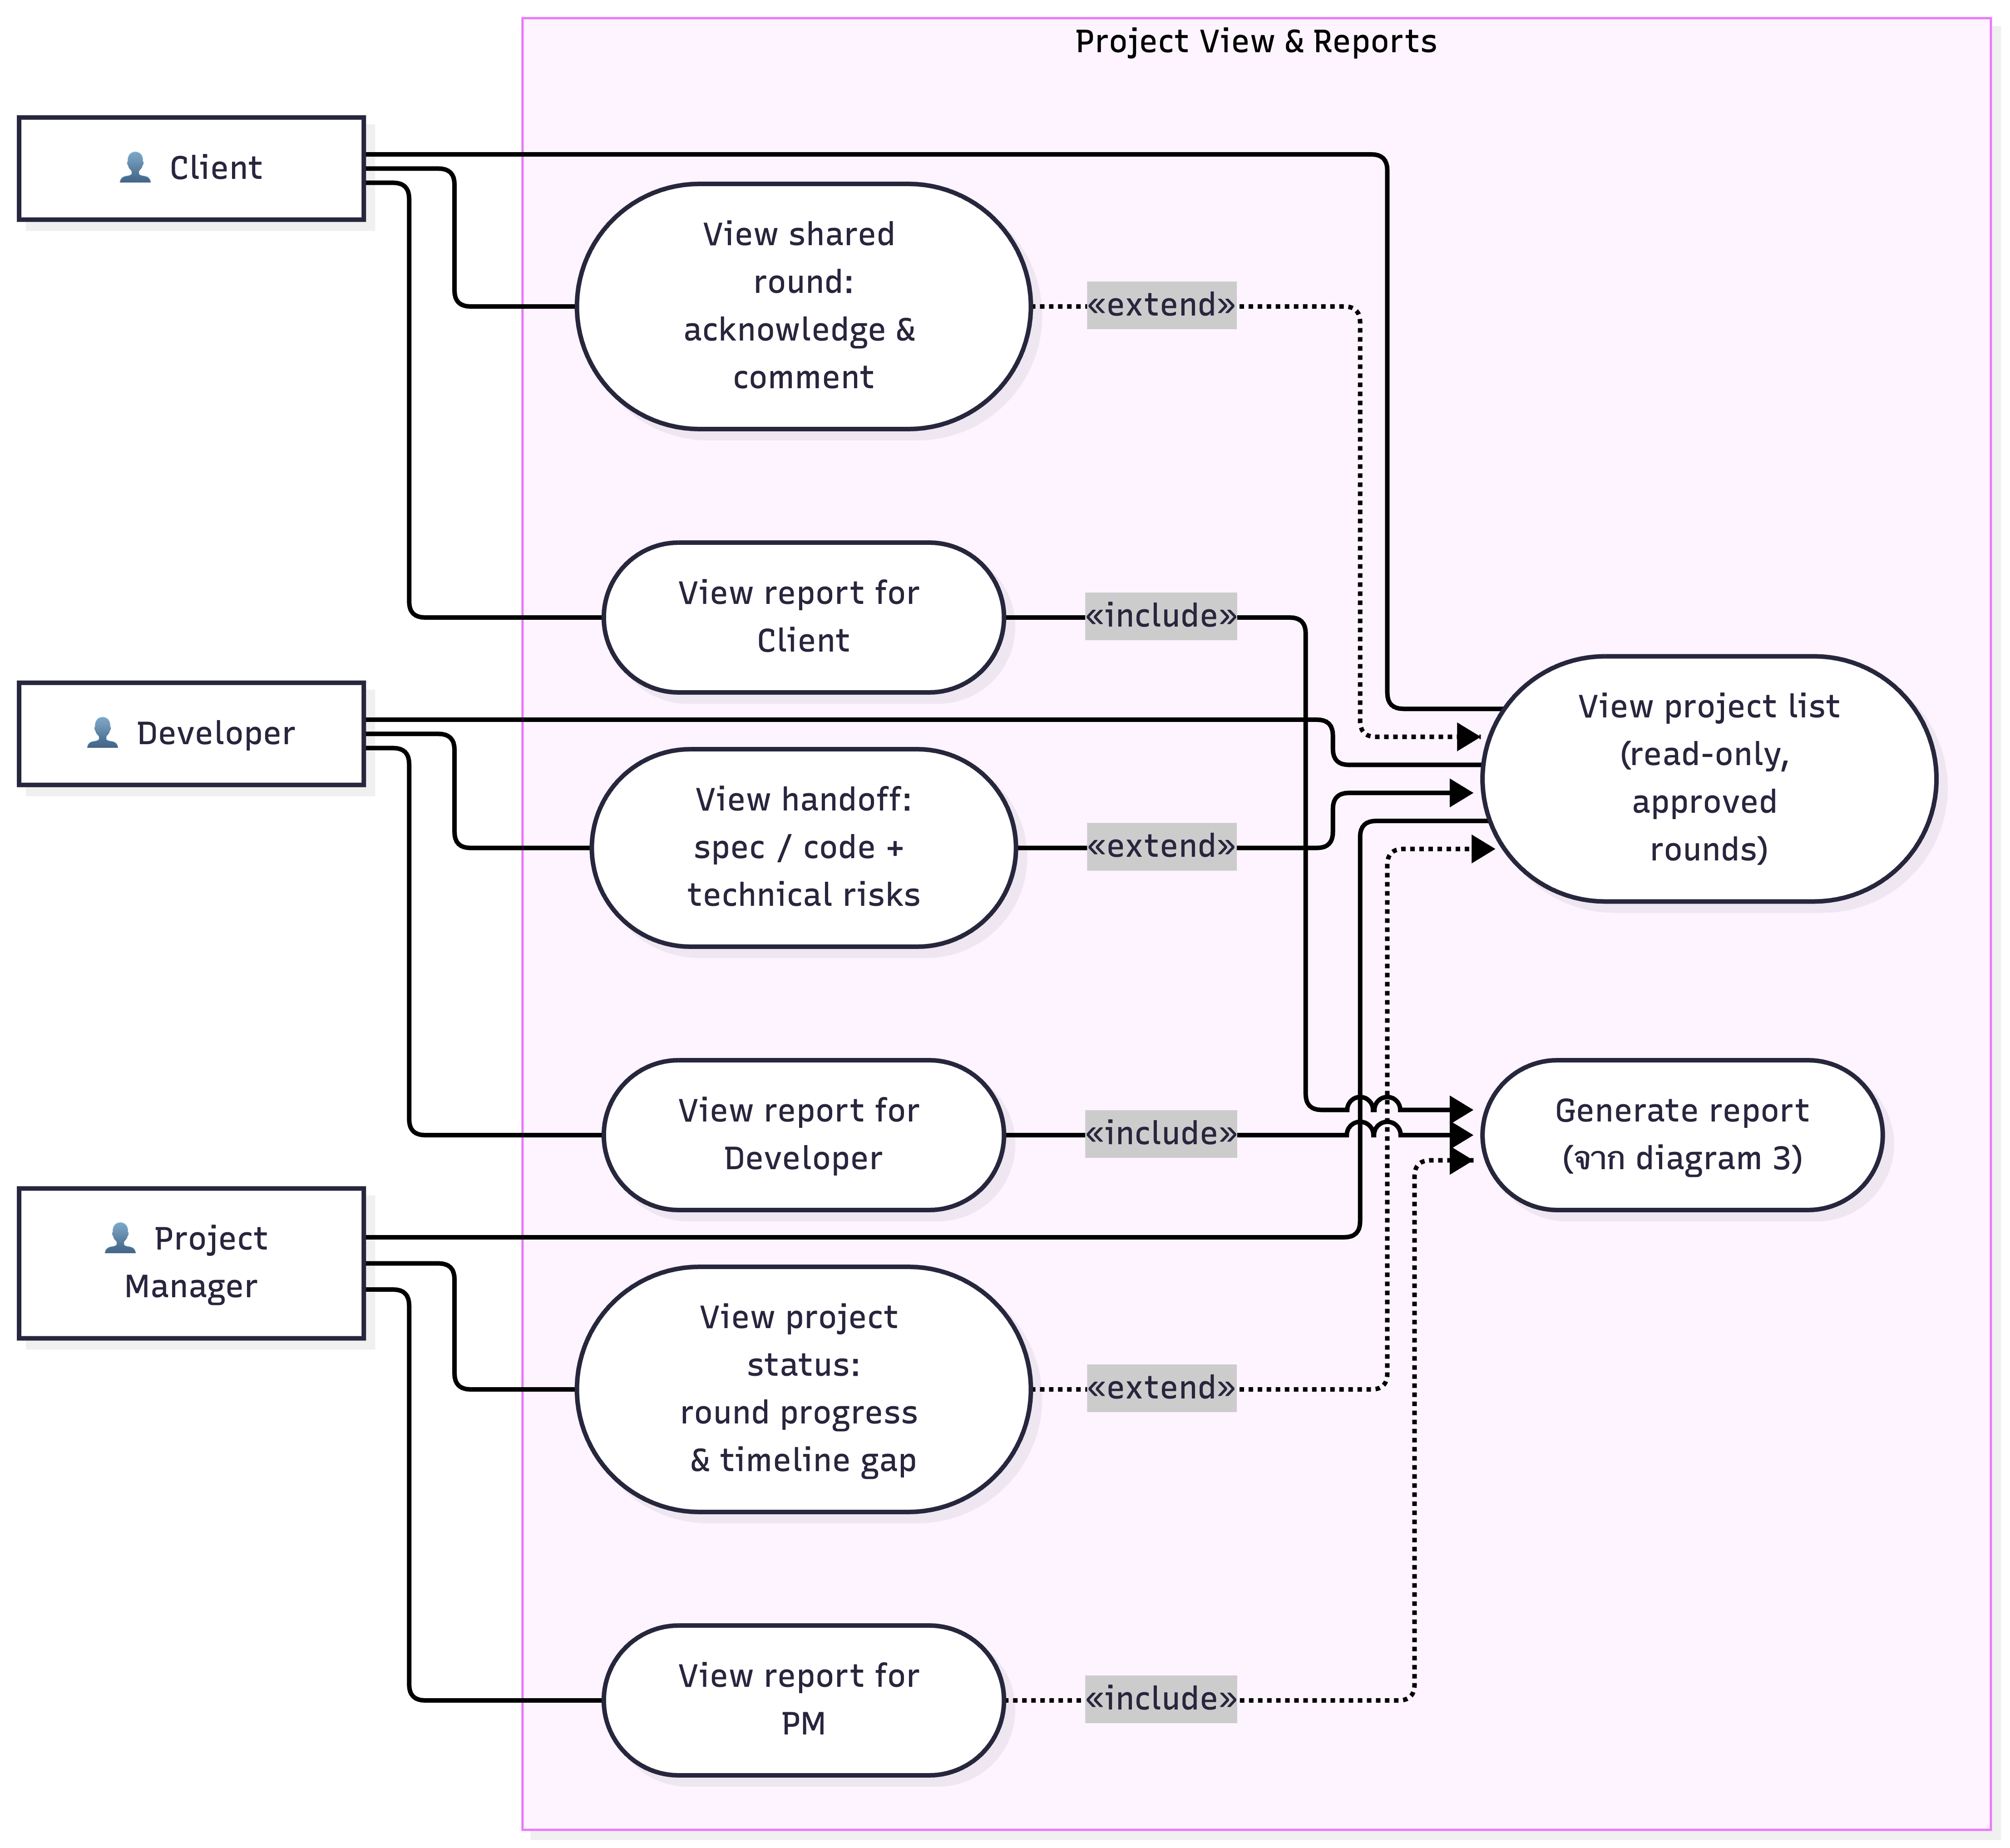
\includegraphics[
      width=0.6\textheight,
      height=\linewidth,
      keepaspectratio,
      origin=c
    ]{figures/ch3-methodology/UC-4.png}
    \caption{Use case diagram for Project view and Report}
    \label{fig:UC-4}
    \thaijustify{
      ภาพแสดง Use Case ของการดูโครงการและรายงาน โดย ผู้ใช้งาน, นักพัฒนา และ ผู้ดูแลโครงการ สามารถดูข้อมูลโครงการที่ได้รับอนุมัติและข้อมูลที่เกี่ยวข้องตามบทบาท รวมถึงดูรายงานที่สร้างจากผลการทดสอบและ Feedback
    }
  \end{figure}
\end{samepage}

\section{System Architecture \& Tech Stack}
\begin{figure}[H]
  \centering
  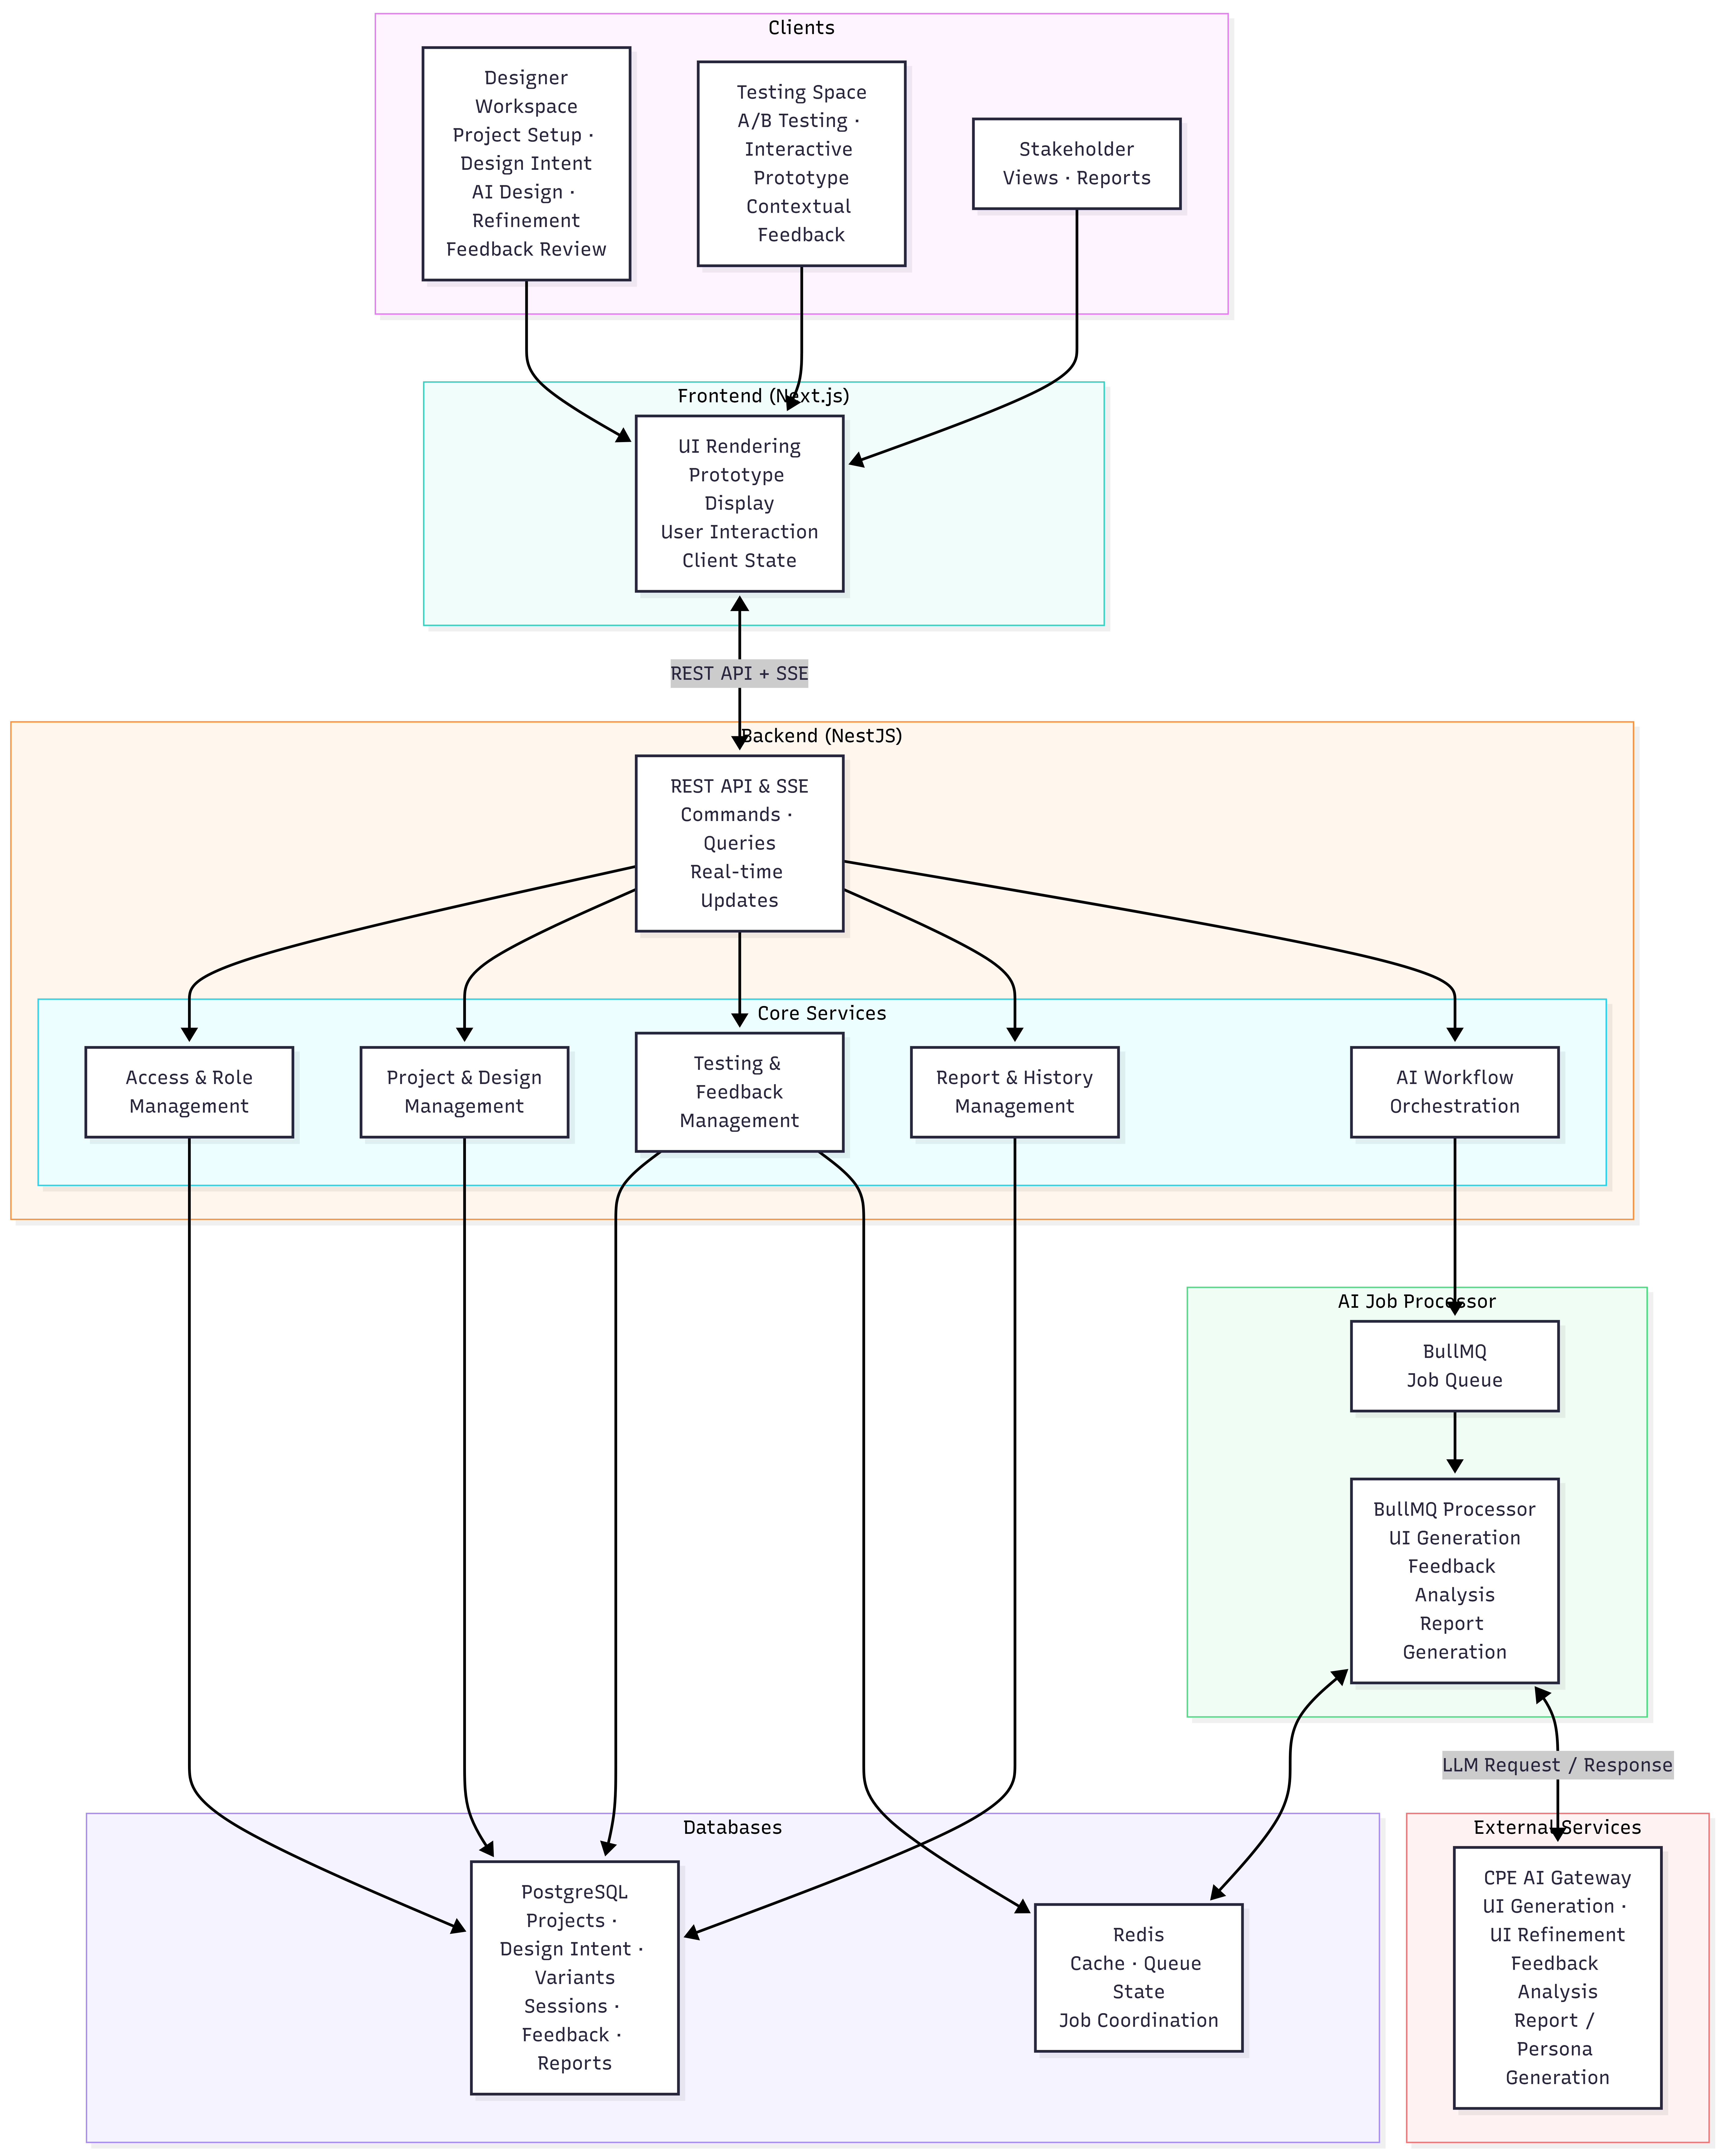
\includegraphics[
    width=0.8\linewidth,
    height=\textheight,
    keepaspectratio
  ]{figures/ch3-methodology/sys-arch3.png}
  \caption{System architecture}
  \label{fig:tech-stack-system-architecture}
  \thaijustify{ภาพแสดงสถาปัตยกรรมระบบโดยแบ่งออกเป็น Client, Frontend, Backend, AI Job Processor, Database และ External Services โดย Frontend พัฒนาด้วย Next.js และสื่อสารกับ Backend ผ่าน REST API และ SSE (Server-Sent Events) ซึ่งช่วยให้ Server สามารถส่งข้อมูลและการอัปเดตแบบ Real-time ไปยัง Client ได้โดยไม่ต้องส่ง Request ใหม่ ขณะที่ Backend ซึ่งพัฒนาด้วย NestJS ทำหน้าที่จัดการสิทธิ์ ข้อมูลโครงการ การทดสอบ Feedback รายงาน และกระบวนการ AI โดยงานที่ต้องใช้เวลาประมวลผลจะถูกส่งผ่าน BullMQ ไปยัง AI Job Processor และเชื่อมต่อกับ CPE AI Gateway สำหรับการประมวลผลด้วย AI}
\end{figure}


% !TeX root = ../../../proposal.tex
% Chapter 4: Results (not written yet)
% \chapter{ผลการดำเนินงาน}
% \thaijustify{
%   [ภาพรวมของบทนี้]
% }
% \section{ผลจากการดำเนินการ}
% \thaijustify{
%   [เนื้อหาในหัวข้อนี้]
% }
% \section{ผลลัพธ์จากการทดลองเปิดใช้งานซอฟต์แวร์}
% \thaijustify{
%   [เนื้อหาในหัวข้อนี้]
% }
% \section{ผลจากแบบสำรวจความพึงพอใจของซอฟต์แวร์}
% \thaijustify{
%   [เนื้อหาในหัวข้อนี้]
% }
% \section{การอภิปรายผลจากการดำเนินการ}
% \thaijustify{
%   [เนื้อหาในหัวข้อนี้]
% }


% !TeX root = ../../../proposal.tex
% Chapter 5: Conclusion (not written yet)
% \chapter{บทสรุป}
% \thaijustify{
%   [ภาพรวมของบทนี้]
% }
% \section{สรุปผลโครงงาน}
% \thaijustify{
%   [เนื้อหาในหัวข้อนี้]
% }
% \section{ปัญหาที่พบและการแก้ไข}
% \thaijustify{
%   [เนื้อหาในหัวข้อนี้]
% }
% \section{ข้อเสนอแนะสำหรับการพัฒนาต่อในอนาคต}
% \thaijustify{
%   [เนื้อหาในหัวข้อนี้]
% }



%%%%%%%%%%%%%%%%%%%%%%%%% Bibliography %%%%%%%%%%%%%%%%%%%%%%%%%
%: Comment this in your report to show only references you have
%: cited. Otherwise, all the references below will be shown.
% \nocite{*}

% Use the kmutt.bst for bibtex bibliography style
% You must have cpe.bib and string.bib in the correct directory
% You may go to file .bbl to manually edit the bib items.

%: Sept, 2021 by Thanin
%: Improve url breaks to prevent unnecessary big white spaces in some cases
\makeatletter
\g@addto@macro{\UrlBreaks}{\UrlOrds}
\makeatother

%: July, 2024 by Jatetanan
%: Add biblatex for managing bibs
%: Uncomment this if you're using biblatex
\printbibliography[heading=bibintoc,title={บรรณานุกรม}]

%: Uncomment \bibliographystyle and \bibliography if you're not using biblatex

%: References style
%: Examples: \bibliographystyle{bibstyle/kmutt}
% \bibliographystyle{bib/ieee}

%: References files
%: Examples: \bibliography{example/string,example/string2,example/cpe}
% \bibliography{bib/codern}

% !TeX root = ../../../proposal.tex
% Appendices
%%%%%%%%%%%%%%%%%%%%%%%%% Appendices %%%%%%%%%%%%%%%%%%%%%%%%%%%
% \appendix{ชื่อภาคผนวก A}
% [เนื้อหาภาคผนวก A]

% \appendix{ชื่อภาคผนวก B}
% [เนื้อหาภาคผนวก B]



\end{document}
%%%%%%%%%%%%%%%%%%%%%%%%%% REPORT END %%%%%%%%%%%%%%%%%%%%%%%%%%%%%%%
